\documentclass[11 pt, letterpaper]{article}
\usepackage{apacite}
\usepackage[margin=1.5in]{geometry}
\usepackage{setspace}
\usepackage{enumitem}
\usepackage{csquotes}
\usepackage{amsmath}
\usepackage{float}
\usepackage{colortbl}
\SetBlockEnvironment{quotation}
%\usepackage[hidelinks]{hyperref}
\usepackage{url}
\usepackage{authblk}
\usepackage{adjustbox}
\usepackage{array}
\usepackage{fancyhdr}
\usepackage{svg}
\usepackage{multirow}
\usepackage{chngpage}
\doublespacing
\usepackage{graphicx}
\usepackage[format=plain,
            labelfont=bf]{caption}






\begin{document}
	
{\begin{titlepage}
		\large
		\singlespacing
		\begin{center}
			\mbox{}
			\vfill
			\textsc{Mapping Inequalities of Access to Employment and Quantifying Transport Poverty in Canadian Cities}\\
			\vfill
			by \\
			\vfill
			{Jeff Allen}\\
			\vfill
			\vfill
			A thesis submitted in conformity with the requirements \\
			for the degree of Master of Arts  \\
			Department of Geography and Planning \\
			University of Toronto \\
			\vfill
			{\copyright} Copyright 2018 by Jeff Allen\\
			\vspace{.01\textheight}
			\mbox{}
		\end{center}
		\setcounter{page}{1}
	\end{titlepage}
	\setcounter{page}{2}}






\renewcommand{\thepage}{\roman{page}}%

\newpage


{
\begin{center}
\section*{Abstract}
	\singlespacing
	{Mapping Inequalities of Access to Employment and Quantifying Transport Poverty in Canadian Cities}\\[2ex]
	{Jeff Allen}\\
	{Master of Arts}\\
	Department of Geography and Planning\\
	University of Toronto\\
	{2018}\\
\end{center}
Millions of Canadians rely on public transportation to conduct daily activities and participate in the labour force. However, many are disadvantaged because existing public transit service does not provide sufficient access to destinations. Limited transit options, compounded with socioeconomic factors like not having a private vehicle, can result in transport poverty, limiting travel to important destinations, like employment opportunities. Accordingly, the objective of this thesis is to develop accurate measures of accessibility to examine the degree to which the Canadian urban population can reach employment opportunities via public transit. These measures are used to analyze inequalities in accessibility with respect to socioeconomic status and estimate where, and to what extent, Canadians are at risk of transport poverty. This knowledge is able to inform policy aimed to increase transit ridership, reduce inequalities of transit accessibility, and limit transport-related barriers to activity participation.

\vspace{12mm}



\newpage



\tableofcontents

\addcontentsline{toc}{subsection}{Table of Contents}

\newpage

\addcontentsline{toc}{subsection}{List of Figures}

\listoffigures

%\listoffigures

\newpage

\addcontentsline{toc}{subsection}{List of Tables}

\listoftables




\newpage

\section*{List of Acronyms \& Abbreviations}

\addcontentsline{toc}{subsection}{List of Acronyms \& Abbreviations}

\begin{tabular}{ l l }
	BRT & Bus Rapid Transit \\
	DA & Dissemination Area \\
	CT & Census Tract \\
	CV & Coefficient of Variation \\
	GIS & Geographic Information Systems \\
	GPS & Global Positioning System \\
	GTA & Greater Toronto Area \\
	GTFS & General Transit Feed Specification \\
	LRT & Light Rail Transit \\
	OSM & OpenStreetMap \\
	OSRM & Open Source Routing Machine \\
	OTP & OpenTripPlanner Routing Engine \\
	SES & Socioeconomic Status

\end{tabular}

\newpage


\renewcommand{\thepage}{\arabic{page}}% Arabic numerals for page counter
\setcounter{page}{1}

\section{Introduction}

Public transit is paramount in providing many urban Canadians with the ability to travel to daily activities and participate in the labour force. Especially within lower income groups, transit is often the only means for accomplishing independent travel in Canada's expanding metropolises. Despite this reliance, many neighbourhoods are disadvantaged because public transit does not provide sufficient access to destinations, like employment opportunities. Poor transit access, combined with other forms of social and economic disadvantage (e.g. poor health, not being able to afford a car, etc.), can result in transport poverty \cite{casas2007,preston2007,lucas2012}. This can limit people in their ability to find employment opportunities and participate in the labour force. The Canadian government is currently investing billions of dollars in public transport, and social equity and inclusion are part of policy goals across the country \cite{canbudget2017}. However, the extent of inequalities in transit accessibility, and the number of people at risk of transport poverty, are unknown at a national scale.

Accordingly, the contributions of this thesis are as follows: 
1) Develop a novel methodology for computing comparative measures of access to employment for Canada's eight largest cities.
2) Analyze the inequalities of transit access to employment in Canada with respect to socioeconomic status.
3) Estimate where, and to what extent, Canadians are at risk of transport poverty.
4) Describe and generate typologies for areas vulnerable to transport poverty in order to recommend urban planning strategies which reduce inequalities and limit the risks of transport-related exclusion.

In generating a comparative measure of access to employment, we account for minute-by-minute variations in transit schedules, competition both among the labour force for jobs as well as employers for employees, and appropriately standardize in order to compare between regions which have different levels of imbalance between the number of jobs and the size of the labour force. We use this formulation to compute access to jobs for Canada's eight largest cities (Toronto, Montreal, Quebec City, Ottawa, Winnipeg, Calgary, Edmonton, and Vancouver). This is computed for travel by transit, as well as travel by car, to allow for modal comparison. We compute this accounting for all jobs within the region, as well as dis-aggregating jobs by income level to examine how access varies among income groups, and to account for how people are more likely to compete for jobs within the same income brackets. We summarize our measures through a series of plots and maps to compare within and between regions.

In examining the inequalities of access, we first analyze the overall distribution of transit provision of each region using Gini coefficients and Lorenz curves. This allows us to examine horizontal equity, how well transit access is distributed among the overall population. We find that the larger cities, Vancouver and Toronto, have the highest levels of access in their centres, but these cities are also the most unequal in terms of how transit access is distributed among their populations. We find that Calgary and Edmonton have the lowest levels of transit access on average. Comparing between mode, we find that the distribution of transit access is more unequal than the distribution of auto access in each city. We then compare how transit access is spatially correlated with the locations of low income populations, those who are more likely to be reliant on transit. We find that lower income areas are generally more centrally located and have relatively higher levels of transit access, and low-density suburban areas, with lower levels of transit access, are typically of higher socio-economic status. Despite this positive outlook in aggregate, there are still a substantial number of low income Canadians who are living in areas with low transit accessibility. We estimate the number of Canadians at risk of transport poverty by counting the number of low income or otherwise vulnerable residents who are living in quantiles of transit access, as well as those residing in areas where transit only provides a small fraction of access compared to driving. We estimate that within Canada's eight largest cities, there are 200,000 individuals living in low income households in the lowest quintile of transit access, and 800,000 individuals living in low income households in areas where transit access provides less than one-fifth the level of access provided by car. 

We then combine the methodological and empirical work in this thesis with guidance from more theoretical literature on accessibility in order to recommend policy and urban planning strategies directed towards improving transit access and reducing risks of transport poverty in Canadian cities. Recommendations include focusing future transit investments in areas which have high concentrations of low-income households and low levels of transit access, intensification and diversity of land-use to increase accessibility and reduce commute distances, as well as a consideration of subsidizing ride-sharing or implementing demand-responsive transit in areas of low density. Doing so would help reduce the risks of transport poverty and social exclusion.

The overall structure of this thesis is as follows; it begins with a detailed literature review on transit accessibility, followed by a description of our data and study areas, detail of the methodology used to compute transit access to jobs, presentation of results with particular focus on the relationship between transit access and income inequalities, and ends with a discussion of results, policy implications, and directions for future work.





\newpage

\section{Background}

\subsection{Urban Transportation \& Accessibility}

A primary function of a city is to provide people the opportunity to participate in daily activities, social interactions, and access to destinations necessary for their well-being. This includes, but is not limited to, access to goods and services, employment opportunities, and social and recreational activities. The concept of accessibility is commonly used to assess these social outcomes of urban transport systems. Accessibility is the ease of reaching destinations, and it is often cited as a key tenant of good urban form \cite{lynch1984}. In modern cities, greater levels of accessibility have been significantly associated with shorter commuting times \cite{kawabata2007}, increased employment rates \cite{merlin2017}, higher activity participation rates \shortcite{paez2009}, it reduces risks of social isolation \cite{garrett1999}, and it can foster social inclusion \cite{lucas2012}.

Accessibility is not just a function of a city's transportation network, it is also a function of land use characteristics (e.g. the relative spatial location of where people live and various activity locations) as well as individual social and economic factors (e.g. can someone afford a private vehicle, are they physically able to walk to a transit stop, etc.) \cite{hanson1982, geurs2004}. Access is also constantly evolving (e.g. land-use patterns change over time; firms open, close, or relocate, etc.) and is subject to daily rhythms (e.g. opening hours of services, road congestion, and transit schedules).

While academics have long been concerned with accessibility \cite{hansen1959}, the common paradigm among practising urban planners and engineers over the past 75 years is to improve mobility. Accessibility is the ease of reaching places, while mobility is the ease of movement \cite{cervero1997}. Within this mobility paradigm, modern transportation planning is often framed around improving economic and environmental outcomes like reducing congestion, curbing emissions, and decreasing commute durations. Reducing commute times on specific routes is often spurred by the parochial vision of residents and politicians who desire mobility improvements in their jurisdictions or travel corridors \cite{knight2004}. 
% People are actors embodied within the networks that they're planning, and are therefore subject to a biased approach to the network's attributes based on their situated knowledge and experiences.

An irony is that planning to increase travel speeds and throughput (i.e. enhancing mobility) has in many cases increased commute distances and durations. With more mobility, the range of what people can potentially access is escalated.
People are willing to travel further distances to destinations like employment due to speed improvements. Land use has become more dispersed as distances can be traversed more quickly. The increased mobility provided by private automobiles has resulted in urban sprawl, and sprawl begot congestion and further demands to mobility (e.g. in the form of more lane abundant motorways) \cite{hanson2004}. Over the past several decades, people are travelling further (both in distance and time) to participate in daily activities (e.g. work, shopping, etc.). For example, in Canada, commute durations increased by 5 minutes on average from 1992 to 2005 \cite{turcotte2005}, and has not declined since \cite{sc2015}. 

Since the rise of the private vehicle, public transit has become a secondary mode in most North American urban regions, due to offering less mobility and access than private vehicles. The benefits of public transit include less environmental impacts, more efficient use of public space, and is more affordable for people to use. As well, public transit provides urban travel for those who are unable, or otherwise choose not to, drive. Public transit is often evaluated through localized metrics like frequency of service, trip times, and proximity to nearby transit stops. While these local and route specific measures are important, they are not holistic. They don't examine the system at the network level. For example, even if someone lives near a transit stop served by a frequent transit route, it won't be beneficial if it does not take them to where they want to go in a reasonable amount of time. Research has shown that providing greater access to destinations by transit is highly correlated with increasing transit ridership \cite{owen2015}, and therefore can reduce the economic and environmental detriments of auto-mobility, as well as provide more opportunity for urban travel for those who are unable to drive. Therefore, measuring transit accessibility is pertinent to evaluate existing deficiencies in transit service and help plans for increasing ridership.




\subsection{Measuring Accessibility}

Modern research on accessibility in transportation geography stems from \citeA{hansen1959} who defined accessibility as the potential of opportunities for interaction. At a basic level, measuring accessibility is concerned with evaluating how well does a city's land use and transport networks provide people the ability to go where they want in a reasonable amount of time. Accessibility is a function transport networks, land use characteristics (e.g. one's location in relation to the distribution of destinations and the spatial organization of transport networks) as well as individual social and economic factors (e.g. can someone afford a private vehicle, are they physically able to walk to a transit stop, etc.) \cite{hanson1982, geurs2004}. Accessibility also has a temporal dimension. The availability of destinations and travel times on transport networks vary over time. For example, shops and services have specific opening hours and transit schedules change depending on time of day and day of the week \shortcite{delafontaine2011,widener2017}.

Methodologically, there are a number of ways in which accessibility has been measured in research and practice \cite{handy1997,geurs2004,kwan1998}. Probably the most common form of access to destination metrics are integral, which measure the sum of opportunities that can be reached from specific location(s) in space \cite{handy1997,kwan1998}. These are typically formulated as follows: 
\begin{equation}
A_{i} = \sum_{j = 1}^{J} O_j f(t_{i,j}) 
\end{equation}
Where $A_i$ is the measure of access for a location $i$. $O_j$ is the number of opportunities at a location $j$. $O_j$ can be interpreted as the attractiveness, or gravitational pull, at location $j$. $f(t_{i,j})$ is a decreasing function of travel cost, $t$, from $i$ to $j$. $t_{i,j}$ is based on one or more impedance factors like travel time or monetary cost. The simplest form of $f(t_{i,j})$ is a threshold indicator, which returns a 0 or 1 whether or not the travel time is less than a threshold. In this case, $A_i$ is interpreted as the number of opportunities (e.g. jobs) that can be reached within a set travel time (e.g. within 30 minutes). Gravity models extend this by using a decay function to weight nearby destinations more than destinations that are further away. Common decay functions used include exponential, Gaussian, and inverse-power \cite{handy1997,kwan1998}. Some studies have also compounded the travel cost with the monetary costs of travel into the impedance factors when conducting transit equity research. For example, \citeA{elgen2016mtl} included the fare prices within transit accessibility measures, finding that access decreased where trips required more than one transit agency, which required paying more than one fare.

These methods have also been expanded to incorporate competition for resources at the destination \cite{weibull1976}. This has been commonly used in measuring access to health services, often formulated as floating-catchment approaches, to output accessibility measures as intuitive metrics like doctors per person \cite{luo2003,delamater2013}. Applied to access to employment, competitive measures can account for how employment opportunities and the labour force are both spatially distributed and overlapping, and that competition can exist among both employers and employees \shortcite{shen1998,geurs2003,kawabata2006}. This process typically involves standardizing the number of jobs at a location, $j$, by the number of people who can access those jobs (i.e. by standardizing by a measure of access to the labour force). Competitive accessibility measures have been shown to be a better predictor of employment outcomes than integral measures which do not consider competition \cite{merlin2017}. Competitive measures are therefore preferable to common accessibility measures when measuring access to employment as they account for both the size and spatial structure of both jobs and the labour force, are more accurate in modelling employment outcomes, and allow for comparing between regions of different sizes \cite{geurs2003}.

Measuring accessibility by public transit is complicated by the temporal variations inherent in transit services. Schedules vary by day of week (e.g. weekday vs. weekend services), time of day (e.g. day vs. night service), and even minute-by-minute (e.g. due to differing headways and wait times). For example, travel time from $i$ to $j$ at 8:05am could vary drastically than at 8:00am if the trip is dependent on a route with a low frequency. To measure accessibility by transit, research has combined transit schedules (recently in GTFS format) with walking network graphs to compute door-to-door trip durations pertaining to specific departure times, and to be inclusive of walking to and from stops, wait times, transfer times, and in-transit travel times. \cite{osullivan2000,lei2010,farber2017}. 

Increased power of computation in recent years has allowed for computing large origin-destination matrices and accessibility measures for many departure times which allows for averaging over set periods, like a morning commute \cite{owen2015,farber2017,conway2017}. For example, \citeA{owen2015} used a continuous accessibility measure to model commute mode share by transit across several American cities. In another study, \citeA{farber2017} used these "transit time cubes" to measure access to employment in the Salt Lake City region in Utah. This strategy has also been used to measure access to supermarkets in Cincinnati \cite{farber2014b} and Toronto \cite{widener2017}. More recent work has developed algorithms or sampling strategies for generating travel times and accessibility measures averaged across a time period, without having to compute travel times at every minute-by-minute interval \cite{conway2017,owen2018}. Other recent research has compared accessibility based on the scheduled transit service to the GPS locations of transit vehicles, finding substantial differences in terms of the spatial patterns of accessibility \cite{wessel2017}.

Accessibility measures are typically either place-based (linked to an area) or person-based (linked to an individual) \cite{miller2007}. Place-based accessibility measures assume that everyone living in a zone has the same level of access. This is subject to aggregation uncertainties (i.e. MAUP), nor does it consider how individual constraints can limit travel \cite{kwan1998,kwan2008}. To model these constraints, person-based measures often use a time geography perspective, to consider that a person's path is constrained by having to be at certain places at certain times during the day (e.g. school, employment), bounding any other potential activity participation by these anchor points \cite{hagerstraand1970}. In terms of access to employment, the set of jobs available to someone could be lessened if someone has additional time constraints (e.g. school, child care, etc.). Person-based measures have also been estimated using utility functions which examine weighing the costs and benefits of travelling and participating in activities at potential destinations. The sum of the choice set of destinations in a utility model can be interpreted as an accessibility metric \cite{handy1997}. While containing more detailed travel considerations than place-based measures, person-based measures typically require specialized travel and time-use surveys \cite{handy1997,miller2007}. These tend to be based on a relatively small sample, and they lack the population and multi-region scope of national surveys like national censuses. As well, a benefit of place-based accessibility measures is that if they are linked with commonly used neighbourhood boundaries like census tracts, they are readily comparable with other aggregate level socio-economic and land-use data that are commonly used by urban planners and researchers.

In a review of accessibility measures, \citeA{geurs2004} argues they should be theoretically sound, be easily communicable, have available data sources to be measured by, and be able to be used in social and economic planning and policy. These guidelines are used in this thesis for generating measures for evaluating the inequalities of transport accessibility in Canadian cities.






\subsection{Inequalities of Urban Transportation}

The distribution of land-use and transportation networks in cities is never spatially uniform. Therefore, access to destinations is never equal among urban populations. Centrally located areas will usually have greater access than those further from the centre due to the clustering of firms and activities. Even if land use was perfectly evenly distributed within a city, periphery areas would have less access as they would be further from the total set of activity destinations than central areas.

While some inequality is inevitable, particularly low levels of accessibility can potentially result in transport poverty. Transport poverty occurs when transport disadvantage (not having access to a car, poor public transit options, etc.) compounds with other forms of potential social disadvantage (unemployment or low income, disability or poor health, etc.) \cite{lucas2012}. Transport poverty is the compounded lack of ability to travel to important destinations and activities. This can result in a decrease of opportunities available, dissuasion to participate in activities, and result in social isolation and even foster social exclusion \cite{garrett1999,casas2007,preston2007,lucas2012}. Social exclusion generally refers to when people are prevented from participating in society and activities necessary for their well-being \cite{litman2003,levitas2007}. For example, in the United States, there is a well documented "spatial mismatch" between the location of suburban jobs and the low-income inner-city labour force, affecting unemployment rates and further abetting poverty in certain neighbourhoods \cite{holzer1991}.

The normative argument for reducing inequalities is often framed through a moral lens of social equity. At a basic level, social equity refers to the fairness with which impacts (i.e. benefits and costs) are distributed. For transport policy, social equity is usually framed and directed towards providing equality of opportunity (e.g. to access destinations) rather than of outcome \cite{litman2003}. However, there is no strict definition of equity across studies that evaluate the social impacts of transport plans and policies \cite{preston2007,martens2012justice,pereira2017}. Recent approaches of social equity in transport have included drawing upon Walzer's \textit{Spheres of Justice} \cite{waltzer1983} and Rawls' \textit{A Theory of Justice} \cite{rawls1971} to advocate for increasing the average accessibility in a region while at the same time reducing the gap between the highest and lowest levels of access \cite{martens2012justice,martens2016,pereira2017}. A core idea from \citeA{rawls1971} is that factors such as being from a low income household should not detriment peoples life chances and opportunities. Applied to accessibility, transport networks should not be insufficient to deter people in their ability to travel to key destinations and participate in activities pertinent to their well-being.

Assessing the equity of transport systems is often approached by framing equity in terms of horizontal or vertical dimensions \cite{litman2002,delbosc2011c,pereira2017}. Horizontal equity is concerned with the distribution of a resource, like transit provision, equally amongst the population. Research focused on horizontal equity have found inequalities of transit access over space (i.e. neighbourhoods have unequal levels of accessibility) or when considering the distribution amongst the overall population (e.g. by measuring the inequalities with Lorenz Curves and Gini Coefficients) \cite{delbosc2011c,martens2012justice, welch2013}.

Vertical equity pertains to the distribution of a resource with focus towards specific groups, often those who are more vulnerable to social or economic exclusion. As it pertains to transportation, vertical equity is often studied in relation to income and social class (e.g. focus on providing public transit to low income neighbourhoods), and with regard to mobility need and ability (e.g. how well are an individual's transportation needs met compared to the overall population) \cite{litman2002,welch2013}. In other words, vertical equity is focused on analyzing the compounding factors that can result in transport poverty. There have been a plethora of studies which have measured differences in inequalities in accessibility among the overall population and comparing with various subgroups, who are potentially more vulnerable to experiencing transport poverty. Some studies have found differing levels of access for minority groups \shortcite{gottlieb2001,parks2004,sultana2005}, recent immigrants \shortcite{blumenberg2008,farber2018}, single-parent families \shortcite{paez2013}, by age cohorts \shortcite{delbosc2011c}, by gender \shortcite{hanson1995,kwan1999}, or by wages and income levels \shortcite{delbosc2011c,fan2012,elgeneidy2016tor}. Other studies have generated combined measures of socio-economic disadvantage at a neighbourhood level to compare with accessibility measures to highlight where gaps in transit access align with social need \shortcite{currie2010,foth2013}.

Research has also shown that available travel mode makes a substantial difference in terms of access to destinations, particularly the disparity between transit riders and those who have regular use of a private vehicle \shortcite{shen1998,benenson2011}. Some studies have found that low-income residents in central parts of cities are not disadvantaged by their relative spatial circumstance (central areas tend to have good access), but instead are disadvantaged by a modal mismatch between the rich and poor \shortcite{taylor1995,blumenberg2004,grengs2010b}. Some have recommended policies aimed at helping those without a vehicle to gain access to them to improve their level of access \shortcite{shen1998,lucas2003,blumenberg2004}. While this may be a potential solution for alleviating transport poverty at a small scale, doing so at a large scale may escalate problems of congestion and emissions.

Because of spatial and temporal variations in land use and urban form, completely equitable transport service, and equal access to destinations in particular, is impossible. Even if it was possible, an equality of outcome should not be the objective. People will inherently have different preferences and values in terms of where they choose to live in reference to what is accessible. However, a common goal of transport policy and planning is to reduce vulnerability to transport poverty and minimize wide-ranging inequalities of access, as well as increase the overall accessibility of a region \cite{seu2003,martens2012justice}, i.e. to make transport more equitable, both horizontally and vertically. There have been a number of academic reviews which have discussed how improving people’s access to key destinations, such as employment, should further be part of transport planning and policy \shortcite{wee2011, papa2014, boisjoly2017}, and the incorporation of social equity and justice into transportation plans and policy \shortcite{karner2013,manaugh2015,martens2016, pereira2017}. A general consensus amongst these reviews is that by investing in public transport to improve accessibility, particularly focused towards those at risk of transport poverty, has the potential to reduce inequalities and foster social and economic inclusion.




\subsection{Access to Employment}

Access to employment opportunities in particular has been a key indicator of evaluating the performance, and examining the social outcomes, of a city's transport network \cite{shen1998,bania2008}. Employment is paramount to preventing social exclusion as it provides the financial ability to support other aspects of life. The ability to obtain and retain employment can depend on a number of factors like education, social network, and size and proximity to the labour market.

Difficulties in finding employment can be compounded if local transit service is ineffective in providing access to destinations in a reasonable amount of time. Several studies have examined how lower levels of transit accessibility can negatively affect employment outcomes. For example, \citeA{sanchez1999} found that access to public transit is a significant factor in determining average labour participation rates in the American cities of Atlanta, Georgia and Portland, Oregon. In a survey in the UK, two out of five unemployed citizens link difficulties in finding employment with the inability to use a car and insufficient public transit options \cite{seu2003}. A study in Sweden found that those living in areas with poor job access in 1991 were adversely affected in finding employment over time during a follow up analysis in 1999 \cite{aaslund2009}. \citeA{allard2002} found that proximity to employment opportunities in the Detroit metro area is associated with a higher probability of working and leaving welfare. Other studies have not found a significant relationship with job access and employment outcomes. For example, \citeA{sanchez2004} found no association between transit access and employment status of welfare recipients in six American cities. 

% Residents who do not have regular access to a private vehicle are more reliant on transit to travel to employment as well as other activities. Many studies have shown substantial gaps between in access to jobs between transit and private vehicle \cite{kawabata2007,grengs2010b,benenson2011,golub2014}.

Several studies have used access to employment to analyze how accessibility is distributed among different income groups and socio-economic status \cite{rau2012,foth2013}. Fewer have examined dis-aggregating jobs by income categories, to examine how access to employment varies among socio-economic strata. The job market will vary depending on ones socio-economic status. Lower-income individuals will most likely not be applying to the same positions as those in higher-income categories, and therefore it is useful to measure access to employment by income group. For example, \citeA{ong1998} measured access to low-wage jobs (where low-wage is the bottom quartile of wages) in Los Angeles, to examine how access impacted welfare recipients in finding employment. \citeA{fan2012} looked at the accessibility gains before and after the introduction of LRT investments in the Twin Cities, Minnesota. They stratified their analysis by income group, looking at access to low, median, and high income jobs, finding that proximity to new transit investments result in increased accessibility to all job types relatively evenly in aggregate, but with some spatial variation. Instead of income level data, some studies have looked at jobs by occupation class, and then extrapolate low-wage workers based on the average wage of the occupation class \shortcite{shen1998,paez2013,elgeneidy2016tor}. However, this does not consider any variation within a category (e.g. a job in food services could range from working in fast food to working in a high end restaurant).

There has also been some research in the United States comparing access to employment between cities. \shortciteA{grengs2010} computes and compares access to employment in Washington, D.C. and San Francisco, finding that Washington provides slightly better access by transit, but San Francisco has much better access by private vehicle. Research by \citeA{kawabata2006} compared access by car between Boston, Los Angeles, and Tokyo to evaluate differences in urban form. A report by \citeA{owen2014}, compares and ranks dozens of American cities based on cumulative access to all jobs within the region, based on morning peak hour commute times. Their work has also subsequently been used to predict mode share \cite{owen2015}. One shortcoming in the above approaches is that they do not account for competition for employment. They compare the number of jobs accessible between cities on a one-to-one basis using cumulative measures, resulting in the largest cities typically also having the highest levels of access, but does not consider the larger population competing for jobs. 

The aforementioned research indicates that measuring access to employment by transit is important to evaluate where and to what extent socially or economically disadvantaged populations also suffer from transportation disadvantage, and are thus at risk of transport poverty. Moreover, measures of transit accessibility are linked with commute mode share \shortcite{moniruzzaman2012,owen2015,boisjoly2016}, indicating that if transit accessibility is increased for a neighbourhood, then it could encourage a mode shift away from private vehicles and have several environmental and economic benefits like reducing congestion and emissions. Mode shifting would however more likely occur for those with relatively lower incomes given the relative impact of cost savings on utility \cite{jara1989}. As well, relatively higher levels of access to jobs has been significantly associated with shorter commuting times, both for drivers and public transit users \cite{kawabata2007}.





\subsection{Canadian Context}

In recent decades, Canada has witnessed a rise in socioeconomic inequalities, and concentrations of poverty, both at a regional level \cite{breau2015rising} and within cities \cite{bolton2012,walks2013,hulchanski2010}.
Research by \citeA{walks2013} highlights trends of increasing income inequality, as well as increased polarization within Canadian cities from 1971 to 2006, with larger cities growing more unequal over time. As well, some evidence has indicated that poverty distributions have become more suburbanized, that increased costs of housing in city centres have pushed lower-income residents to more affordable, but less accessible areas. In comparing changes in poverty distributions in Canadian cities from 1986 to 2006, \citeA{ades2012} found that concentrations of poverty have developed in more peripheral urban areas.

% rewrite
% Bourne  (1989)  showed  how  poverty  and unemployment were concentrated in Canadian inner  cities  in  1986.
% Similarly,  Broadway  (1992)  observed  an  overrep-resentation  of  disadvantaged  populations  in  ar-eas   surrounding   the   downtown   core   in   seven Canadian  central  cities.

At the same time, governments and land developers alike have continued the auto-oriented suburbanization process by building highways and sprawling low-density greenfield developments. From 1971 to 2016, the area of built-up urban land in Canada has increased at a greater rate than the growth in urban population \cite{sc2016}. Concurrently, commute times and road congestion have increased in Canadian cities \cite{turcotte2005,metrolinx2008}. From 1992 to 2005, the mean commute duration across Canada's six largest cities increased by 5 minutes on average according to the General Social Survey \cite{turcotte2005}, and have not shown decline \shortcite{sc2015,higgins2017}. Commute times are, on average, the highest in Toronto, Montreal, and Vancouver \cite{turcotte2011,higgins2017}. Commute durations are particularly longer for transit riders. From the 2016 census, the average commute time in Canadian cities by car was 24 minutes, but for transit it was 44 minutes \cite{sc2016}.

Moreover, several Canadian research projects have found that people living in areas with low accessibility have significantly lower activity participation rates, particularly for those who are socially disadvantaged in other ways. For example, \citeA{mccray2007} examined how transportation factors limit the daily activity patterns of low income women in Quebec City. \citeA{spinney2009} showed there is significant association between transport mobility benefits and quality of life for elderly Canadians. \citeA{allen2018} analyzed how low accessibility limits the on-campus participation of University students. A series of papers by \citeA{paez2009} used large-scale travel surveys and spatial econometric models of travel behaviour to identify how the disparities in accessibility among low income, elderly, and single-parent families dissuaded participation in daily activities.

The Canadian government is currently investing billions on transit, in aims to relieve congestion, reduce travel times, and increase accessibility. The 2016 federal budget pledged \$3.4 billion towards transit investment over the subsequent three years, and in 2017 the Canadian government announced it will invest \$20.1 billion over the next decade in public transit through bilateral agreements with provinces \cite{canbudget2017}. Provincial and municipal governments are also investing substantially in transit infrastructure projects. Social equity and inclusion are also increasingly a part of policy goals in regions across the country, as well at a national level \cite{canbudget2017}. However, the range of inequalities in accessibility, and the extent of transport poverty are unknown at a national scale.

Existing research in analyzing transit availability and accessibility have been primarily focused in Canada's two largest cities, Toronto and Montreal. Most of the existing studies have involved comparisons of transit accessibility over time. \citeA{foth2013} examined changes in accessibility from 1996 to 2006 in Toronto and linked this with a synthetic indicator of socio-economic status. They found that more socially disadvantaged neighbourhoods tend to have better transit access relative to the rest of the region, and that the range in accessibility declined over the 10 year period. \citeA{farber2017g} looked at potential changes to accessibility before and after proposed transit infrastructure investments in the Greater Toronto and Hamilton areas. Two other recent studies examined the daily fluctuations in accessibility measures in Toronto. \citeA{elgeneidy2016tor} analyzed how transit access to employment varies in the morning peak period compared to other times during the day, including breakdown by a measure of neighbourhood socio-economic status and a binary classification of low-wage jobs. \citeA{boisjoly2016} expanded upon this research to examine the propensity and differences in daily accessibility measures to model transit mode share for commuting. \citeA{elgen2016mtl} generated a measure of access to jobs in Montreal which incorporates both travel time and transit fare cost, finding that access decreases for trips that incorporate multiple transit agencies. There is a dearth of research in cities other than Montreal and Toronto.

One shortcoming from this existing work is that transit accessibility is typically only measured for single departure times, rather than averaged over a wider period, and therefore does not account for minute-by-minute fluctuations in transit travel times. Computing accessibility for only a single departure time could potentially over or under estimate travel times to employment centres, and thus accessibility scores for certain neighbourhoods \cite{owen2015,farber2017,conway2017}. 

The overall findings from existing research in Canada is that lower income neighbourhoods generally have equitable, and sometimes better, transit access to jobs than the overall population. Results are however most likely skewed by the number affluent suburban neighbourhoods with poor transit access. Wealthier households often choose to live in transit poor neighbourhoods as they have their own vehicles and desire larger property sizes and dwelling units. American studies have shown that after controlling for occupation class, those living further away from employment tend to have higher wages, partly to offset the costs of longer commute times \cite{madden1985}. As well, social housing and lower-income rental buildings are often planned to be sited in areas with relatively better transit. 

However, even though most of the previous research finding that transit access is higher overall for lower income groups, there are still potentially large numbers of low income suburban households lacking sufficient access to jobs. Moreover, this could be increasing due to escalating income polarization in Canadian cities, and rising housing costs, pushing lower-income residents to areas with worse transit service \cite{ades2012}. A report on social inclusion in transport planning in Canada estimated that a third or more of households in Canada have at least one member who is transport disadvantaged \cite{litman2003}. And while ample research has linked transport disadvantage with activity participation and well-being \cite{spinney2009,paez2009}, there is little existing detailed knowledge on the scope of the transport poverty problem, and how it is distributed within and between Canadian cities. This means that existing policy does not have a clear understanding of how to funnel transit investment into projects that reduce inequalities in transit accessibility. The following sections detail the analysis of measuring transit accessibility and quantifying the extent of transit inequalities and transport poverty in Canada's eight largest cities.



\newpage

\section{Study Areas \& Data}

\subsection{Study Areas}

This study looks at the eight most populous urban regions in Canada. Some of these regions consist of multiple adjacent municipalities. Additively, these have been referred to as urban megaregions \cite{simmons2013}. From the 2016 Canadian census, 58\% of Canadians live in these eight regions. Each region has a population of at least 750,000, while no other region in Canada has a population of more than 500,000.

\begin{figure}[H]
	\vspace{4mm}
	\caption{Location of study areas} 
	\label{canada}
	\centerline{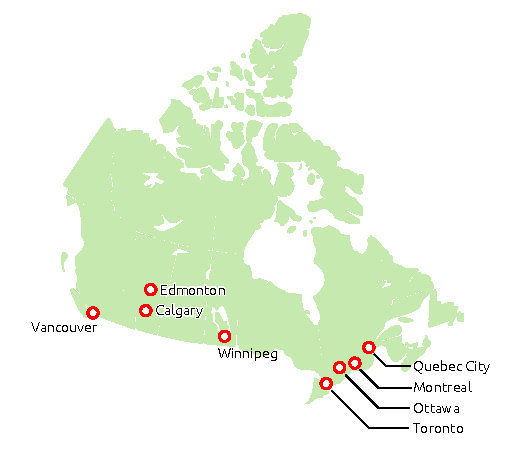
\includegraphics[width=4in]{figures/canada/canada.pdf}}
	\vspace{1mm}
\end{figure}

The boundaries of these urban regions for our analysis are Census Metropolitan Areas (CMA). CMAs are agglomerations of municipalities which pertain to urban areas with a population of over 100,000 where at least 50\% of the employed labour force works in the region's core, as determined from commuting data from the previous census \cite{sc2016cdic}. Although not perfect, this measurement provides consistency of what constitutes the boundaries of urban regions across Canada. For our analysis, any adjacent CMAs are merged into one urban region due to the commuting flow and transit agencies that link adjacent regions. Table \ref{desc_table} provides summary statistics for each of these regions. Two periphery CMAs within the Toronto region, Brantford and Peterborough, were not included as they did not have transit schedules available in a machine readable data format.

\begin{table}[H]
	\vspace{4mm}
	\begin{adjustwidth}{-.25in}{-.25in} 
		\renewcommand{\arraystretch}{0.75} % Default value: 1
		\small
		\caption{Summary statistics by urban region}
		\label{desc_table}
		\begin{tabular}{p{19mm} | p{10mm} p{15mm} p{14mm}  p{14mm} p{21mm} p{12mm} p{12mm}}
			\multirow{2}{*}{} & Area & \multirow{2}{*}{Population} & \multirow{2}{*}{Jobs$^\S$} & Labour & Transit Mode & \multicolumn{2}{l}{Mean Commute Time$^*$} \\ \arrayrulecolor{lightgray}\cline{7-8}
			\arrayrulecolor{black}
			
			& ($km^{2}$)  &  &       & Force$^\S$ &  Share$^\dagger$  & Auto  & Transit \\
			\hline
			Toronto  & 12,160 & 8,335,444 & 3,462,100 & 4,524,570 & 18.4\%  & 29.0  & 49.2 \\
			Montreal & 4,605 & 4,098,927 & 1,756,640 & 2,189,115 & 22.2\%  &  26.8  & 44.4 \\
			Vancouver  & 4,935 & 2,745,461 & 1,091,405 & 1,498,535 & 18.7\%  & 27.2 & 43.8 \\
			Calgary  & 5,110 & 1,392,609 & 587,280 & 816,385 & 15.9\%  & 24.1 & 41.6 \\
			Ottawa  & 6,770 & 1,323,783  & 595,950 & 727,160 & 20.1\%  & 24.7 & 42.2 \\
			Edmonton & 9,440  & 1,321,426  & 553,660 & 758,150 & 11.3\%  & 24.2  & 40.2  \\
			Quebec City & 3,410  & 800,296 & 375,720  & 437,325 & 11.3\% & 21.2  & 35.1 \\
			Winnipeg & 4,310 & 778,489 & 344,320  & 424,250 & 13.4\%  & 22.6 & 35.7 \\
			
		\end{tabular}
	\end{adjustwidth}
	\vspace{-6mm}
	\begin{flushleft}
		\singlespacing\small{
			$^\dagger$ Percent of work commute trips by transit
			
			$^*$ In minutes
			
			$^\S$ Jobs are only those in the region with a "usual place of work" according to the census, while the labour force also includes the unemployed, those who work at home, and those without a fixed place of work.
		}
		
	\end{flushleft}
\end{table}

The three largest regions (Toronto, Montreal, and Vancouver), have a combination of rapid transit, regional rail and bus lines, and local transit service, and are each served by multiple transit agencies. Within each of these three regions, each municipality runs its own transit agency, and there is a regional transit agency providing longer distance bus or train service linking municipalities. Transit trips requiring routes operated by multiple agencies typically require multiple fares. The transit agencies in the central municipalities (Toronto Transit Commission (TTC), Translink in Vancouver, Soci\'et\'e de Transport de Montr\'eal (STM)) each operate both rapid and surface transit, and offer more frequent, greater coverage, and better connectivity than transit agencies in the surrounding, more suburban, municipalities. Regional transit service in these three cities tends to be more focused on commuting trips rather than other types of daily trips like shopping or social activities.

Transit in the Albertan cities of Calgary and Edmonton are each primarily operated by a single transit agency. Both Calgary and Edmonton operate a few Light Rail Transit (LRT) lines, and run surface bus routes. Ottawa-Gatineau has a series of Bus Rapid Transit (BRT) routes alongside local bus services. Quebec City and Winnipeg are primarily only served by surface bus routes which share the road with private vehicles. There has been recent upgrade of a few routes to include dedicated bus lanes (e.g. the Southwest Transitway in Winnipeg). Several cities also have ferries which contribute to the transit with the region. Quebec city has a ferry crossing the St. Lawrence river, Toronto has ferries connecting downtown to its islands, and Vancouver a series of water taxis in False Creek and the Sea Bus which links downtown to North Vancouver. A summary of the CMAs and transit agencies included in each of the eight regions is provided in Table \ref{table_cma_agencies}.

\newcolumntype{L}[1]{>{\raggedright\let\newline\\\arraybackslash\hspace{0pt}}m{#1}}

%p{12mm}p{8mm}p{14mm}p{33mm}p{60mm}
\begin{table}
	\vspace{4mm}
	\begin{adjustwidth}{-.25in}{-.25in} 
		\begin{singlespace}
		\renewcommand{\arraystretch}{1.2} % Default value: 1
		\small
		\caption{Summary of CMAs and Transit Agencies used in this study}
		\label{table_cma_agencies}
		\begin{tabular}{L{19mm}L{10mm}L{17mm}L{33mm}L{60mm}}
			           & Area ($km^{2}$) & Population & CMAs                                                                                                  & Transit Agencies                                                                                                                                                                                                                                                                                                                                                                                                                          \\
			\hline
			Toronto$^\dagger$    & 12,160 & 8,335,444& Oshawa, Toronto, Hamilton, St. Catharines-Niagara, Kitchener-Cambridge-Waterloo, Guelph, Barrie & Toronto Transit Commission, Durham Regional Transit, GO Transit, York/VIVA, MiWay, Brampton Transit, Oakville Transit, Burlington Transit, Hamilton Street Railway, Niagara Region Transit, Guelph Transit, Barrie Transit, Grand River Transit, Toronto Island Ferries                                                                                                           \\ \hline
			Montreal*   & 4,605  & 4,098,927    & Montreal                                                                                & Agence métropolitaine de transport, CIT Chambly-Richelieu-Carigna, CIT du Haut-Saint-Laurent, CIT La Presqu'île, CIT Laurentides, CIT Le Richelain, CIT Roussillon, CIT Sorel-Varennes, CIT Vallée-du-Richelieu, CRT Lanaudière, MRC de Deux-Montagnes, MRC de L'Assomption, MRC Les Moulins (Urbis), Réseau de transport de Longueuil, RTM Sud-ouest, Societe de transport de Laval, Société de transport de Montréal, OMIT Sainte-Julie \\ \hline
			Vancouver   & 4,935  & 2,745,461    & Vancouver, Abbotsford-Mission, Chilliwak                                                              & BC Transit, TransLink, West Coast Express                                                                                                                                                                                                                                                                                                                                                                                                 \\ \hline
			Calgary     & 5,110  & 1,392,609    & Calgary                                                                                               & Calgary Transit, Airdie Transit                                                                                                                                                                                                                                                                                                                                                                                                           \\ \hline
			Ottawa      & 6,770  & 1,323,783    & Ottawa - Gatineau                                                                                     & OC Transpo, Société de transport de l'Outaouais                                                                                                                                                                                                                                                                                                                                                                                           \\ \hline
			Edmonton    & 9,440  & 1,321,426    & Edmonton                                                                                              & Edmonton Transit Service, Fort Sask Transit, St. Albert Transit, Strathcona County Transi                                                                                                                                                                                                                                                                                                                                                 \\ \hline
			Quebec City & 3,410  & 800,296     & Quebec City                                                                                           & Réseau de transport de la Capitale, Société de transport de Lévis                                                                                                                                                                                                                                                                                                                                                                         \\ \hline
			Winnipeg    & 4,310  & 778,489     & Winnipeg                                                                                              & Winnipeg Transit                                                                                                                                                                                                                                                                                                                                                                                                                         
		\end{tabular}
	\end{singlespace}
	\end{adjustwidth}
	\vspace{-6mm}
	\begin{flushleft}
	\singlespacing\small{
		$^\dagger$ Toronto region does not include periphery municipalities of Peterborough or Brantford due to transit data being unavailable
		
		$^*$  Montreal region does not include the periphery municipality of Saint-Jean-sur-Richelieu due to transit data being unavailable
		
		
	}
	
	\end{flushleft}

\end{table}

\subsection{Demographic \& Employment Data}

Within these urban regions, we use 2016 census Dissemination Areas (DA) to model the home locations of the labour force. DAs are the smallest areas in which socio-economic data is available from the quinquennial Canadian census, minimizing error due to the modifiable areal unit problem (see \citeA{kwan2008} for a discussion of MAUP and its effects in accessibility research). DAs are designed and delineated for populations of 400 to 700 persons \cite{sc2016cdic}, and have been used in other studies on transit accessibility in Canada \cite{widener2017,wessel2017}. Specifically, we use the population weighted centroids of DAs snapped to the closest walking network segment to model the home locations of residents. Larger, neighbourhood sized Census Tracts (CT), however, are used for the location of employment, as they are the lowest level in which complete employment data was available for the 2016 census. It should be noted that several of these urban regions also run their own travel surveys (e.g. the Transportation Tomorrow Survey in the Toronto Region) with home and employment locations of residents, but we required data collected with consistent methodology across the country. Regional travel surveys typically have much more detailed travel diaries, but survey a lower percent of the overall population. The long-form census, which we draw our data from, is a 25\% representative sample of Canadian households. 

To analyze in relation to socio-economic status, we use individual and household demographic and income data from the 2016 Canadian census. Income data from the 2016 census is based on yearly income from 2015, the full calendar year prior to the national survey \cite{sc2016cdic}. Included in this is a count of low-income households. These are households which have 50\% or less than the median adjusted after-tax income of all households and includes an adjustment to account for household size. It should also be noted that some DAs in our areas of study have suppressed data because of low populations or low response rates. These DAs are omitted from subsequent analysis (2\% of DAs in our study regions, but only 0.5\% of the overall population). %Table \ref{sumstats} provides a summary of population counts and basic commuting stats for each of the eight urban regions.





\subsection{Network Graphs}

Another primary input into our analysis are travel times by transit linking where people live and places of employment. To compute these travel times, we built custom multi-modal network graphs for each urban region. These graphs are inclusive of the time walking to and from stops, wait times, in-vehicle travels times, and transfers. These were built using the open-source routing engine \citeA{otp}. This has two sets of inputs. The first are the walking networks in each of these cities via the topological edges from OpenStreetMap. The second are transit schedules in the form of GTFS (General Transit Feed Specification) data for every transit agency that serves these urban regions, circa May 2016 in order to align with the collection dates of the 2016 census. OTP uses the $A^\text{*}$ algorithm to find shortest-path transit itineraries between each origin and destination, and can be parameterized to set limits on overall travel time, walk distances, number of transfers, and wait times \cite{otp}. It should be noted that GTFS represents the expected schedules generated by transit agencies, while the on-the-ground service of vehicles often differs from the schedule, and can potentially effect accessibility measures in some urban areas \cite{wessel2017}. Real-time GPS data of transit vehicles is not available for all the agencies in our study regions, so this was not feasible for this project.

To provide comparison to transit travel times, we also compute travel times by driving, using OpenStreetMap data as the input network. The travel times for driving were computed with a different routing engine, Open Source Routing Machine (OSRM) \cite{luxen-vetter-2011}, as it includes greater consideration for driving attributes like speed limits, turn restrictions, and one-way streets.



\newpage

\section{Measuring Access to Employment}

\subsection{Computing Travel Times}

The first step of our analysis was to compute travel time matrices of DAs (home locations) to CTs (employment locations) for each of the eight urban regions in our study. Because of the inherent temporal variations in transit schedules, we follow the precedent in the literature to compute transit travel times for every minute of the morning commute period \cite{owen2015,farber2017}, to be subsequently averaged when computing accessibility metrics. Figure \ref{travel_time_morning} exemplifies how travel time by transit between a residential neighbourhood and an employment centre can vary substantially, and selecting one of these travel times could greatly over- or under-estimate the travel time during this period.

\vspace{4mm}
\begin{figure}[H]
	\caption{Example of the temporal differences in commute time by transit from a residential neighbourhood to a mall in northwestern Toronto} 
		\label{travel_time_morning}
	\centerline{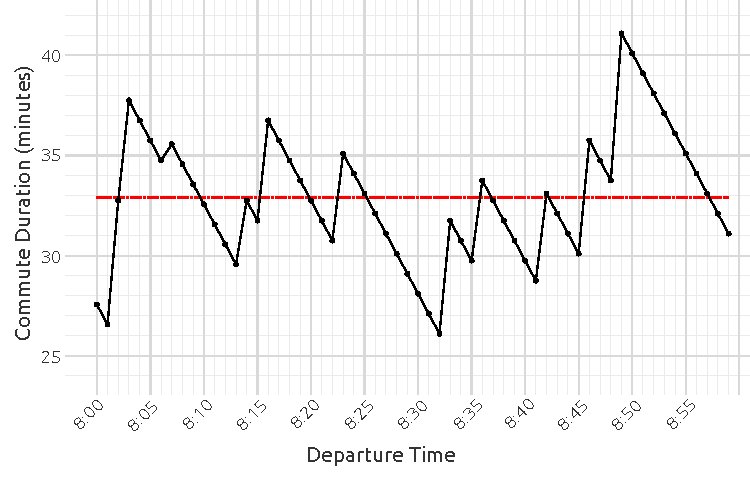
\includegraphics[width=5in]{figures/trip_time_dept/trip_time_dept.pdf}}
	\vspace{2mm}
\end{figure}


%fFFFFFFFFFF2 shows how the area accessible by transit within a 30 minute commute varies depending on the . Such variation can. 

For our analysis, this was computed in parallel over several processing units which output results for multiple departure times, $\tau$. The outputs are stored in a three-dimensional array. 
\begin{equation}
T_{i,j,\tau} = \begin{Bmatrix}{t_{i,j,\tau}}\end{Bmatrix}
\end{equation}
Where each cell, $t_{i,j,\tau}$, is the travel time from the origin DA, $i$, to the destination CT, $j$, for a specific departure time, $\tau$. Due to heavy computation, travel times were capped at 90 minutes, assuming that no one would be willing to travel to jobs that require more than a 90 minute commute.

Due to a lack of openly available network level congestion data, travel times for driving were computed as free-flow speeds, and then multiplied by a congestion factor, $k_c$, to account for how peak-hour travel is slower than off-peak. The congestion factors were set at 1.7 for Toronto and Vancouver, 1.6 for Montreal, 1.5 for Ottawa, and 1.4 for the remaining four cities. These values were estimated from reports examining costs of congestion in Canadian cities \cite{metrolinx2008,cong2012} as well as from the private data vendor TomTom, which hosts an online worldwide ranking of congestion by city \cite{tomtom2018}. We also apply a minor two minute penalty for parking, $t_p$. The peak hour travel time by driving between two locations, $t_{i,j,d}^*$, is thus calculated from the free flow travel time, $t_{i,j,d}$, as follows.
\begin{equation}
t_{i,j,d}^* = k_c \hspace{1mm} t_{i,j,d} + t_p
\end{equation}




\subsection{Cumulative Accessibility}

The first, and simplest, measure of accessibility we compute is cumulative accessibility. This is the count of employment opportunities that can be reached within a specified travel time, $\theta$, and is formulated as follows

\begin{equation}
A_{i,\theta} = \sum_{j = 1}^{J} O_j f(t_{i,j},\theta) 
\end{equation}
$O_j$ is the number of job opportunities at location $j$.  $f(t_{i,j},\theta) $ is a binary function of whether the travel time from $i$ to $j$ is less than a travel time threshold, $\theta$.

\begin{equation}
f(t_{i,j},\theta) = 
\begin{cases} 
1 \hspace{3mm} \text{if} & t_{i,j} \leq \theta \\
0 \hspace{3mm} \text{if}  & t_{i,j} > \theta
\end{cases}
\end{equation}
Because of the inherent continuous temporal variations in transit schedules, we average these measures over the morning rush hour period (from $\tau_a$ to $\tau_b$)
\begin{equation}
\bar{A}_{i,\theta} = |\tau_b - \tau_a|^{-1} \int_{\tau_a}^{\tau_b} A_{i,\theta} (\tau) d\tau
\end{equation}
%=|M|^{-1} \sum_{m \in M} \sum_{j = 1}^{J} O_j f(t_{i,j,m,\theta}) 
Since we computed travel times at a per minute basis, $\bar{A}_{i,\theta}$ can be generalized as follows.
\begin{equation}
\bar{A}_{i,\theta} = |120|^{-1} \sum_{\tau \in M} \sum_{j = 1}^{J} O_j f(t_{i,j,\tau,\theta})
\end{equation}
Where $M$ is every minute $\tau$ from 7:00am to 8:59am. Figure \ref{cumacc_time} exemplifies how departure time can seriously effect accessibility measures, and why averaging is beneficial.

The output can also be highly sensitive to $\theta$, particularly for $t_{i,j}$ which are close to the threshold. For example, for $\theta = 30$, an opportunity 29 minutes away is counted, but an opportunity 31 minutes away is not, even though the difference between these is only two minutes travel time. To test sensitivity due to parameter selection, we compute cumulative accessibility at fifteen minute intervals from $\theta = 15$ minutes to $\theta = 90$ minutes to allow for more detailed comparative analysis.


\vspace{4mm}
\begin{figure}[H]
	\caption{Differences in cumulative accessibility by departure time for a dissemination area (dauid = 46110663) in Winnipeg} 
	\label{cumacc_time}
	\centerline{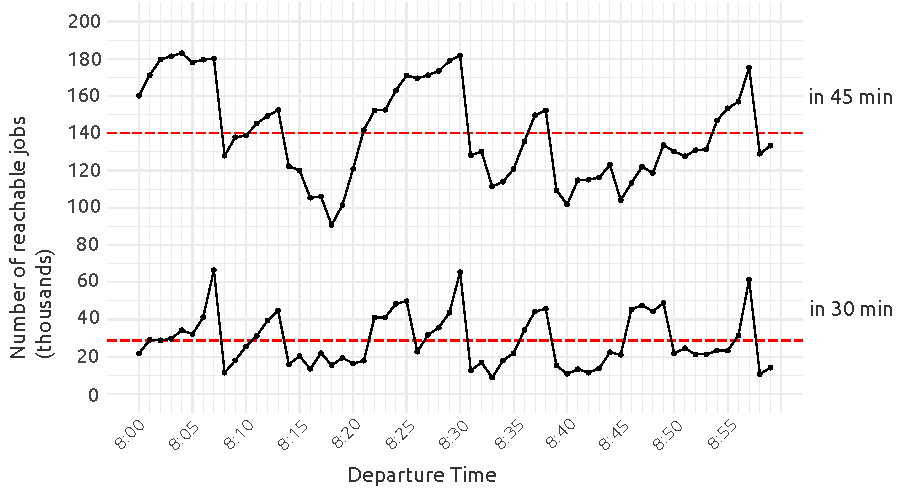
\includegraphics[width=6in]{figures/time_cumulaccess/time_cumacc.pdf}}
	\vspace{2mm}
\end{figure}





\subsection{Gravity Accessibility}

While cumulative accessibility measures are relatively simple to understand, they do not account for how job opportunities nearby are more attractive than those further away due to the time savings resulting from reduced commute durations. To account for this, we also compute gravity measures of accessibility where the function, $f(t_{i,j})$, weights nearby opportunities more than those that are further away via decay functions.

Commonly used formulations include Gaussian, exponential, and inverse-power functions \cite{handy1997,osullivan2000}. The formulation used can lead to varying results and conclusions \cite{guy1983,kwan1998}. For our study, we compute access to jobs using an inverse-power function and an exponential decay function, both parametrized such that a 30 minute commute returns a value of 0.5, and with a maximum value of 1 (at $t_{i,j} = 0$). 30 minutes is approximately the average commute duration across all eight regions \cite{sc2016}. Figure \ref{gravity} displays these two functions, comparing them with a simple linear decay function as well as a cumulative measure with $\theta = 45$. The two decay functions have very similar trajectories from 0 to 30 minutes, but afterwards, the inverse-power functions decays more rapidly, reaching 0 at $t_{i,j} = 90$. In terms of access to jobs, this means that the two functions would weight nearby jobs similarly, but the exponential function would weight further away jobs more than the inverse-power function. 

\begin{figure}[H]
	\vspace{4mm}
	\caption{Gravity functions} 
	\label{gravity}
	\centerline{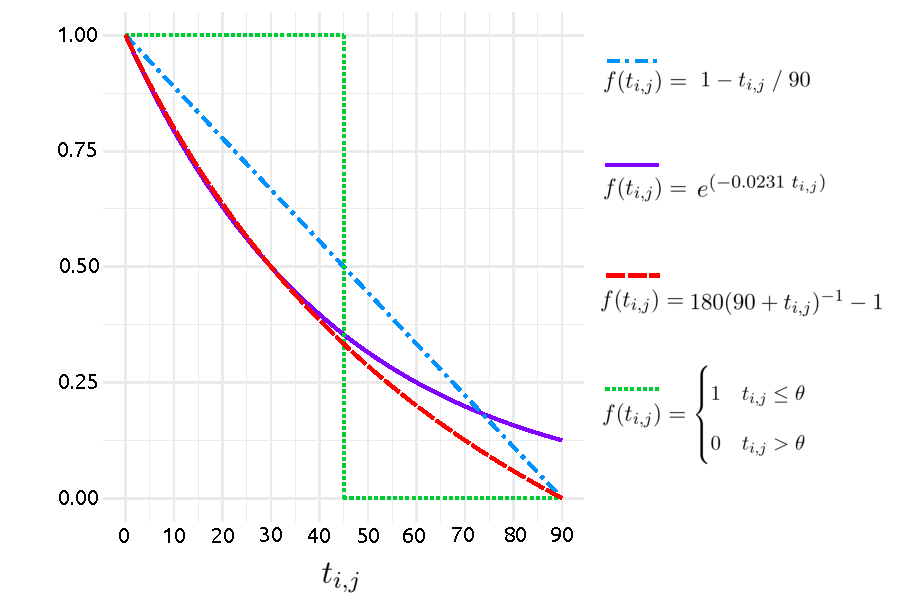
\includegraphics[width=5in]{figures/gravity/gravity.pdf}}
	\vspace{2mm}
\end{figure}



\subsection{Competitive Accessibility}

Gravity and cumulative measures of access to jobs are inadequate when comparing results both within and between cities because they do not account for the size and spatial distribution of the labour market which competes for employment opportunities \cite{shen1998}. For example, central Toronto may have tenfold the amount of nearby jobs than central Winnipeg, but if the nearby labour force is ten times the size, then access should be approximately equivalent if there is an equal number of jobs per worker.

To account for this, we also computed competitive measures of accessibility. This technique accounts for access at both the demand and supply locations of analysis \cite{weibull1976}, and has been commonly used in access to health services \cite{luo2003,delamater2013}. Applied to access to employment, this accounts for how employment opportunities and the labour force are both spatially distributed and overlapping, and that competition exists among the labour force for employment opportunities \shortcite{shen1998,allard2002,kawabata2006}. Moreover, competitive accessibility measures have been shown to be a better predictor of employment outcomes than accessibility measures that do not consider competition \cite{merlin2017}. Mathematically, this technique involves normalizing employment opportunities at $j$ by their labour market catchment area, $L_j$ (i.e. this is the demand for jobs at $j$).

\begin{equation}
A_{i} = \sum_{j = 1}^{J} \frac{ O_j f(t_{i,j})}{L_{j}}
\end{equation}
\begin{equation}
L_j = \sum_{i = 1}^{I} P_i f(t_{i,j})
\end{equation}
Where $P_i$ is the labour force at $i$. If gravity functions are used for $f(t_{i,j})$, then the units of the output values from the above equations however are not easily discernible. In research on access to health services, this metric has been simplified by setting $f(t_{i,j})$ as an indicator function with a threshold in order to output measures as population to provider ratios for different areas (these are commonly referred to as 2-step floating catchment area measures) \cite{luo2003,delamater2013}. Most previous studies utilizing a competitive accessibility metric for measuring access to employment have only considered a two-step approach \shortcite{shen1998,allard2002,wang2002,sanchez2004,kawabata2006,rau2012}. However, this two-step process does not take into account how each $P_i$ has varying levels of access, but can only fill a set amount of jobs. i.e. employers compete for workers who have varying levels of access to jobs, just as people compete for jobs at locations which have varying access to the labour force \cite{geurs2003}. This can be formulated from theory on spatial interaction modelling, specifically using the balancing factors of a doubly constrained model. Typically in a doubly constrained interaction model, balancing factors are used to ensure that the sum of flows from $i$ and destined to $j$ equals the observed amount arriving and departing from each zone \cite{wilson1971,fotheringham1989}. To port this theory into computing measures of accessibility, $A_i$ is incorporated into the equation for $L_j$ to normalize for the number of opportunities that someone at location, $i$, can reach  \cite{geurs2003,merlin2017}.

\begin{equation}
A_{i} = \sum_{j = 1}^{J} \frac{ O_j f(t_{i,j})}{L_{j}} 
\end{equation}
\begin{equation}
L_j = \sum_{i = 1}^{I} \frac{ P_i f(t_{i,j})}{A_{i}}
\end{equation}

Because $L_j$ and $A_i$ are mutually dependent, they have to be estimated iteratively. To exemplify this iterative process, let's contemplate a simplistic linear city with three residential areas ($a,b,c$) and two employment zones ($x,y$) (see Figure \ref{S1}).

\begin{figure}[H]
	\caption{Example city for measuring competitive accessibility} 
	\label{S1}
	\centerline{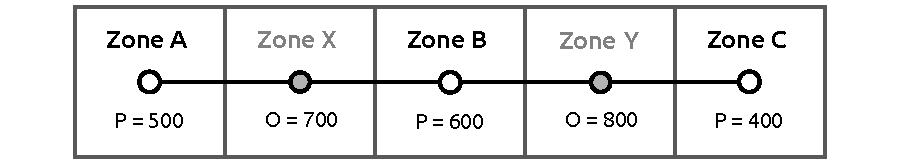
\includegraphics[width=5in]{figures/linear_city/linear_city_S1.pdf}}
	\vspace{2mm}
\end{figure}

Furthermore, lets assume that this is a closed system, that there is an equal number of jobs and workers in the region, and that workers can only travel to adjacent zones (e.g. people in zone $a$ cannot travel to employment opportunities in zone $y$). Without accounting for competition, the number of jobs accessible given these constraints are $A_{a} = 700$, $A_{b} = 1500$, and $A_{c} = 800$. However, looking at Figure \ref{S1}, we see that population is tipped to the left, while employment is tipped to the right, leading to the presumption that there is less competition for the jobs in zone $y$ than in zone $x$. Let's now compute access considering competition. To begin, we compute $L_j$, assuming that all residential zones have equal levels of access (i.e. $A_a = A_b = A_c = 1$)

\begin{equation}
\begin{array}{l}
L_{x} = 500 / 1 + 600 / 1 = 1100 \\
L_{y} = 600 / 1 + 400 / 1 = 1000
\end{array}
\end{equation}

We find that employers at location $x$ have a greater labour force within its catchment area than at location $y$, by a difference of 100 workers. We then account for this when computing $A_i$ (e.g. this is a basic 2-step floating catchment measure of access). 

\begin{equation}
\begin{array}{l}
A_{a} = {700}/{1100} = 0.636 \\
A_{b} = {700}/{1100} + {800}/{1000} = 1.436\\
A_{c} = {800}/{1000} = 0.800
\end{array}
\end{equation}

Most previous studies utilizing a competitive accessibility metric have only considered a 2-step approach \shortcite{shen1998,sanchez2004}. However, as we will see, $A_i$ can change after another iteration after it is used to recompute $L_j$, in order to take into account the variation in access achieved by the labour force.

\begin{equation}
\begin{array}{l}
L_{x} = {500}/{0.636} + {600}/{1.436} = 1203.4 \\
L_{y} =  {600}/{1.436} + {400}/{0.800} = 917.7
\end{array}
\end{equation}

\begin{equation}
\begin{array}{l}
A_{a} = {700}/{1203.4} = 0.582 \\
A_{b} = {700}/{1203.4} + {800}/{917.7} = 1.453\\
A_{c} = {800}/{917.7} = 0.872
\end{array}
\end{equation}
Notice how the values of $A$ have either increased or decreased. Simulating this scenario for 10 iterations finds results converge to the limits of 0.5, 1.0, and 1.5

\vspace{4mm}

\begin{figure}[H]
	\caption{Convergence of $A_i$ for the scenario presented in Figure \ref{S1} }
	\label{S1c}
	\centerline{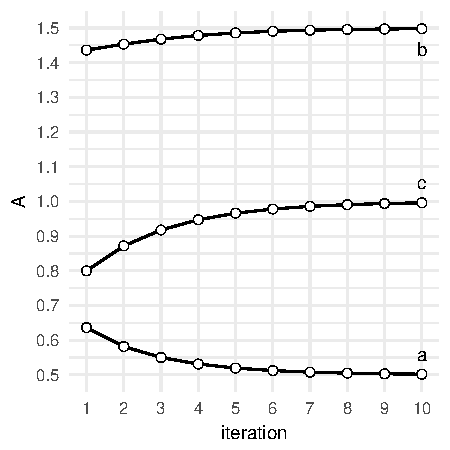
\includegraphics[width=3in]{figures/convg/conRS1.pdf}}
	\vspace{2mm}
\end{figure}

Without this approach, i.e. just looking at access without competition results in $A_{a} = 700$, $A_{b} = 1500$, and $A_{c} = 800$. The access to employment for $a$ and $c$ were initially approximately half of $b$. However, when we account for competition, $A_{c}$ is two-thirds of $A_b$, while $A_a$ is one-third of $A_b$. As well, $A_c$ is double $A_{a}$, while without competition, their access levels were closer to being equal. Additionally, there is substantial difference between the first iteration, and the result we get after iterating (e.g. moving from 0.8 to 1.0 for zone $c$, and from 0.636 to 0.5 for zone $a$). Therefore, not iterating can result in over or underestimating accessibility for certain zones.

Given that the total jobs in the region equals the sum of the labour force, then the measures will converge, with a mean approximate to one (i.e. there is one job for every worker in the region). Yet in real world cases, the number of job opportunities rarely equals the size of the labour force within a region. This could be due to workers commuting in and out of the region, unemployed individuals being part of the labour force who are also competing for jobs, people working multiple jobs, or an urban economy with an excess of job opportunities that remain unfilled. Lets examine the situations where there is an imbalance between jobs and workers within a region, starting with more jobs than workers. For example, expanding upon our first scenario, lets presume that a new employer opens an office in $x$, providing 100 more jobs to the region.

\begin{equation}
\sum_{j = 1}^{J} O_j \hspace{2mm} > \hspace{2mm} \sum_{i = 1}^{I} P_i
\end{equation}
\begin{figure}[H]
	\caption{Example scenario where there are more jobs than workers}
	\label{S3}
	\centerline{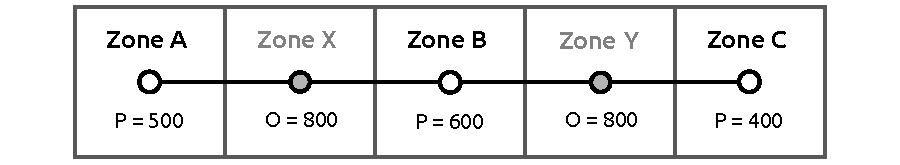
\includegraphics[width=5in]{figures/linear_city/linear_city_S3.pdf}}
\end{figure}
We see in Figure \ref{S3c} (left) that the magnitude of $A_i$ increases after each iteration. However, when standardized (right), they converge. 
\begin{figure}[H]
	\caption{Convergence of the scenario presented in Figure \ref{S3}}
	\label{S3c}
	\centerline{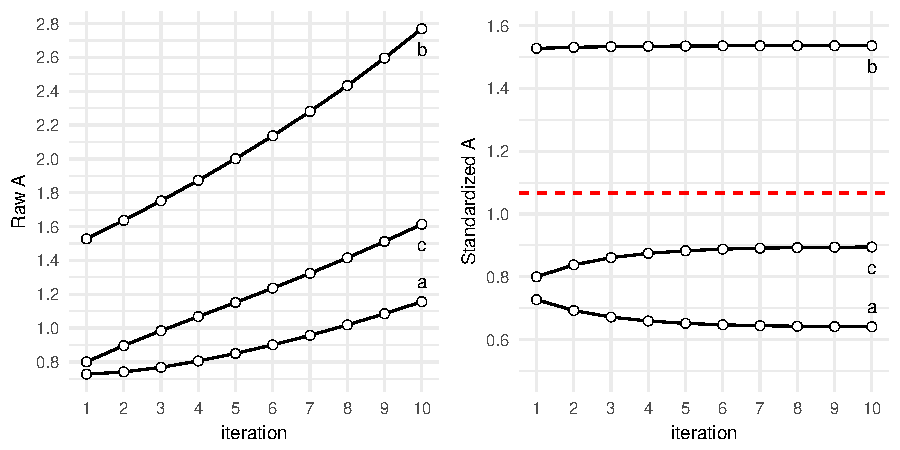
\includegraphics[width=6in]{figures/convg/conRS3.pdf}}
	\vspace{2mm}
\end{figure}
The values in this case are standardized using the mean accessibility of the population observed after the first iteration. This allows $A_i$ to be interpretable as an ersatz jobs per person metric. The equation for $A_i$ is updated as follows to incorporate this standardization.

\begin{equation}
A_{i} = \frac{\bar A_o}{\bar A_c} \sum_{j = 1}^{J} \frac{ O_j f(t_{i,j})}{L_{j}} 
\end{equation}

Where $\bar A_c$ is the population mean after an iteration $c$, and $\bar A_o$ is the population mean after the first iteration. The population mean level of access is computed as follows.

\begin{equation}
\bar A = \frac{\sum_{i=1}^{I} P_i A_i}{\sum_{i=1}^{I} P_i}
\end{equation}

The mean in Figure \ref{S3c} (red line) is greater than one since there are more jobs than workers in the region in this scenario.

Alternatively, if the labour force is greater than the number of jobs in the region, then the values of $A_i$ decline after each iteration, but again, if standardized, they converge. Figures \ref{S4} and \ref{S4c} show the result after adding 100 people to the labour force to each of the three residential zones. The mean in Figure \ref{S4c} is less than one as there are more potential workers than jobs within the region.

\begin{equation}
\sum_{j = 1}^{J} O_j \hspace{2mm} < \hspace{2mm} \sum_{i = 1}^{I} P_i
\end{equation}
\begin{figure}[H]
	\caption{Example of where the labour force is greater than the number of jobs} 
	\label{S4}
	\centerline{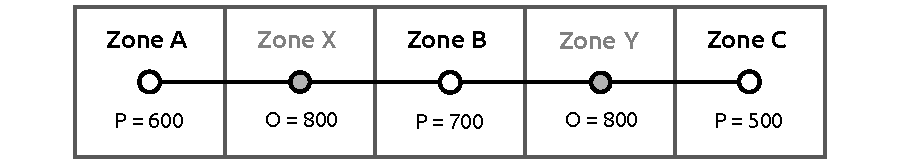
\includegraphics[width=5in]{figures/linear_city/linear_city_S4.pdf}}
\end{figure}
\begin{figure}[H]
	\caption{Convergence of the scenario presented in Figure \ref{S4}} 
	\label{S4c}
	\centerline{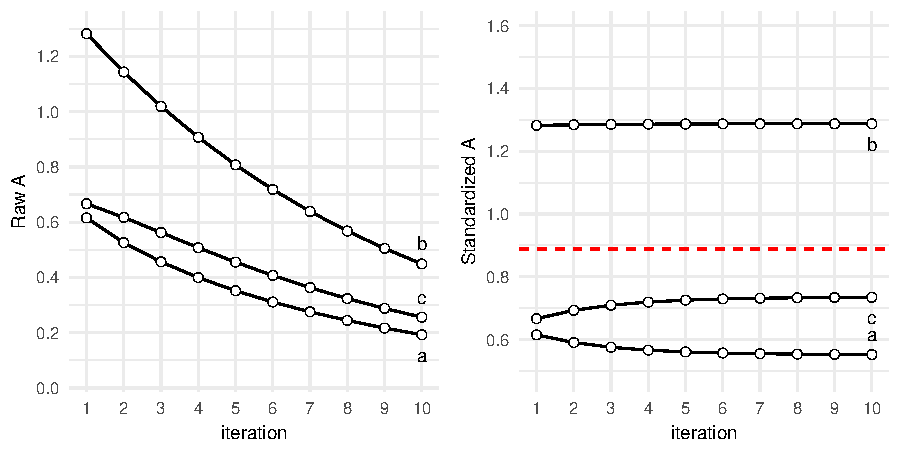
\includegraphics[width=6in]{figures/convg/conRS4.pdf}}
\end{figure}

The above models, however, do not allow for adequate comparison between cities. For example, lets presume there are two cities, each with the same distribution of jobs and workers, but the separation between zones in one city is half than in the other city (Figure \ref{S6}). For these scenarios, $f(t)$ is an inverse function of the travel time (the greater $f(t)$ the shorter the travel time). However these two scenarios will result in the same measures of accessibility, even though $f(t)$ is doubled.

\vspace{1mm}
\begin{figure}[H]
	\vspace{1mm}
	\caption{A comparison of two cities} 
	\vspace{1mm}
	\label{S6}
	\centerline{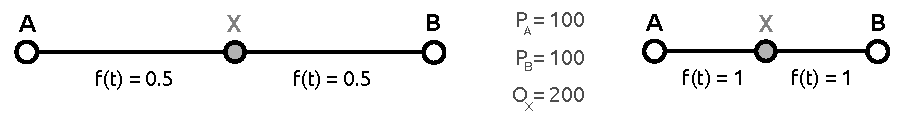
\includegraphics[width=5in]{figures/linear_city/linear_city_2.pdf}}
\end{figure}
\[
\begin{array}{ll}
\textbf{City 1} & \hspace{2mm} \textbf{City 2} \\
L_{x} = 100 (0.5) + 100 (0.5) = 100 & \hspace{2mm} L_{x} = 100 (1) + 100 (1) = 200 \\
A_{a} = 200 (0.5) / 100 = 1 & \hspace{2mm} A_{a} = 200 (1) / 200 = 1 \\
A_{b} = 200 (0.5) / 100 = 1 & \hspace{2mm} A_{b} = 200 (1) / 200 = 1 \\
\end{array}
\]
\vspace{1mm}

Access for $a$ and $b$ in both scenarios are equal to one. The magnitude of the travel times are inconsequential, only the relative values matter within each system. This conundrum was highlighted by \citeA{delamater2013} in using floating catchment areas to measure access to health services. For our study, this distinction is important because we wish to make comparisons between cities, using the same units of travel time impedance. Yet cities have differences within their transport network structure, offering varying levels of mobility and travel times between locations. To account for this in access to health services, \cite{delamater2013} adds an additional $f(t_{i,j})$ term in the equation for $A_i$ to account for both the relative and absolute distances between $i$ and $j$.

\[
\begin{array}{ll}
\textbf{City 1} & \hspace{2mm} \textbf{City 2} \\
\text{Step 1} & \hspace{2mm} \text{Step 1} \\
L_{x} = 100 (0.5) + 100 (0.5) = 100 & \hspace{2mm} L_{x} = 100 (1) + 100 (1) = 200 \\
A_{a} = 200 (0.5)(0.5) / 100 = 0.5 & \hspace{2mm} A_{a} = 200 (1)(1) / 200 = 1 \\
A_{b} = 200 (0.5)(0.5) / 100 = 0.5 & \hspace{2mm} A_{b} = 200 (1)(1) / 200 = 1 \\
\bar A_o = 0.5 & \hspace{2mm} \bar A_o = 1 \\
\text{Step 2} & \hspace{2mm} \text{Step 2} \\
L_{x} = 100 (0.5) / (0.5) + 100 (0.5) / (0.5) = 200 & \hspace{2mm} L_{x} = 100 (1) / (1) + 100 (1) / (1) = 200 \\
A_{a} = 200 (0.5)(0.5) / 200 = 0.25 & \hspace{2mm} A_{a} = 200 (1)(1) / 200 = 1 \\
A_{b} = 200 (0.5)(0.5) / 200 = 0.25 & \hspace{2mm} A_{b} = 200 (1)(1) / 200 = 1 \\
\bar A_c = 0.25 & \hspace{2mm} \bar A_c = 1 \\
A_{a} = (0.5 / 0.25) 0.25 = 0.5 & \hspace{2mm} A_{a} = (1 / 1) 1 = 1 \\
A_{b} = (0.5 / 0.25) 0.25 = 0.5 & \hspace{2mm} A_{b} = (1 / 1) 1 = 1 \\
\end{array}
\]

The scenario on the left returns half the level of accessibility than the scenario on the right, due to having half the $f(t)$.

Furthermore, in most cities, people travel to work by different travel modes, and compete for jobs within a multi-modal labour force \cite{shen1998,sanchez2004}. For example, a job at $j$ would be more attractive for someone at $i$, if they have regular access to a private vehicle and the commute by car from $i$ to $j$ is less than by transit. Therefore, we need to expand the measure of $L_j$ to account for multiple modes (i.e. the labour force that can reach $j$ will be a combination of those who travel by transit and car).

\begin{equation}
L_j = \sum_{\forall \lambda \in \Lambda} \sum_{i = 1}^{I} \frac{ \alpha_{i,\lambda} P_i f(t_{i,j,\lambda})}{A_{i,\lambda}}, \hspace{8mm}
\sum_{\forall \lambda \in \Lambda} { \alpha_{i,\lambda} = 1}
\end{equation}

Where $\alpha_{i,\lambda}$ is the mode share for travel to work trips of the labour force at location $i$ and $t_{i,j,\lambda}$ is the travel time from $i$ to $j$ for the mode, $\lambda$. Access to jobs for a travel mode, $\lambda$, can therefore be computed as follows.

\begin{equation}
A_{i,\lambda} = \frac{\bar A_0}{\bar A_c} \sum_{j = 1}^{J} \frac{ O_j f(t_{i,j,\lambda}) f(t_{i,j,\lambda})}{L_{j}} 
\end{equation}

As well, the formula for the population mean level of access is updated to account for multiple modes.

\begin{equation}
\bar A = \frac{\sum_{\forall \lambda \in \Lambda} \sum_{i=1}^{I} \alpha_{i,\lambda} P_i A_{i,\lambda}}
{\sum_{i=1}^{I} P_i}
\end{equation}

The measures of $A_{i,\lambda}$ will either rise or decline after each iteration, depending on the mobility the mode provides relative to other modes, as well as the mode share for different zones. Let's go back to our original example, and examine differences between transit and auto accessibility.

\begin{figure}[H]
	\hspace{2mm}
	\caption{Example city for measuring competitive accessibility} 
	\label{S5}
	\centerline{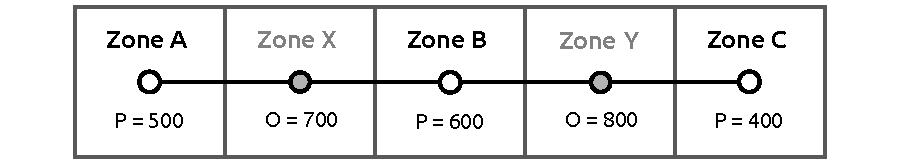
\includegraphics[width=5in]{figures/linear_city/linear_city_S1.pdf}}
	\vspace{2mm}
\end{figure}

Let's assume that half the population in each zone travels by transit, and the other half by private vehicle ($\alpha = 0.5$). Also, let's assume that the impedance function for travel time to the adjacent zone for transit is half than that by driving (i.e. $f(t_T) = 0.5$ and $f(t_D) = 1.0$). Figure \ref{S5c} shows the converging output, which results in transit riders having half the level of access than motorists in their respective zones. As well, the relative difference between zones also remains the same as the output from the first scenario. For example, location $c$ has twice the level of accessibility than location $a$, when looking at either transit or auto mode share.

\begin{figure}[H]
	\caption{Convergence of the example in Figure \ref{S5} with two travel modes (red is by transit, white is by car)} 
	\label{S5c}
	\centerline{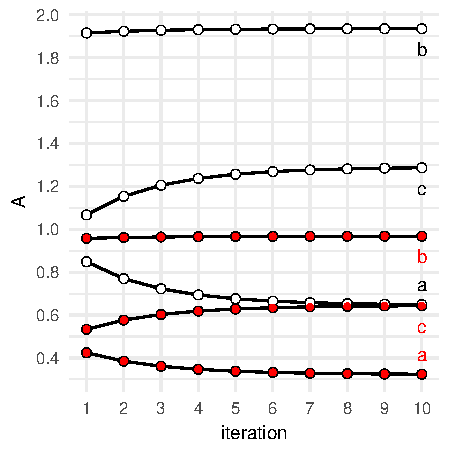
\includegraphics[width=3in]{figures/convg/conRS5.pdf}}
	\vspace{2mm}
\end{figure}


For our study of Canadian cities, we generalize the above formulas to account for driving and transit mode share, including averaging transit over the morning commute period because of fluctuations in the transit schedules.

\begin{equation}
A_{i,T} = |120|^{-1} \sum_{\tau \in M} \frac{\bar A_0}{\bar A_c} \sum_{j = 1}^{J} \frac{ O_j f(t_{i,j,\tau}) f(t_{i,j,\tau})}{L_{j}}
\end{equation}
\begin{equation}
A_{i,D} = \frac{\bar A_0}{\bar A_c} \sum_{j = 1}^{J} \frac{ O_j f(t_{i,j,d})  f(t_{i,j,d})}{L_{j}}
\end{equation}
\begin{equation}
\bar A = \frac{\sum_{\forall \lambda \in \Lambda} \sum_{i=1}^{I} \alpha_{i,\lambda} P_i A_i}{\sum_{i=1}^{I} P_i}
\end{equation}
\begin{equation}
L_j = |120|^{-1} \sum_{\tau \in M} \sum_{i = 1}^{I} \frac{ \alpha_{i,T} P_{i} f(t_{i,j,\tau})}{A_{T,i}}
+ \sum_{i = 1}^{I} \frac{\alpha_{i,D} P_{i} f(t_{i,j,d}) }{A_{D,i}}
\end{equation}
$A_{i,T}$ is the accessibility measure for transit, and $A_{i,D}$ for driving. $t_{i,j,d}$ is the travel time by driving during the commute period. $f(t_{i,j,\tau})$ and $f(t_{i,j,d})$ utilize an inverse-decay function. $\alpha_{i,D}$ is the commute mode share ratio of workers at location $i$ who travel to work via private vehicle. $\alpha_{T,i}$ is the mode share ratio by transit and walking. The mode share for transit for our study is assumed as the total non-driving commuting population ($\alpha_{i,T}$ = 1 - $\alpha_{i,D}$), and therefore also includes the small percent of those who take active modes (bike or walk). This assumes that those who bike or walk to work are also able to commute to work by transit, but not by car. 

These measures are computed both for the overall labour force and employment opportunities as well as dis-aggregating by income level. When computing dis-aggregate measures, $P_i$ and $O_j$ pertains both to workers and jobs within a specific income range. The income ranges are split at \$10,000 intervals as this is how Statistics Canada tabulates and releases their data \cite{sc2016cdic}. We have to assume that the lower-income or unemployed portion of the labour force has the same mode split as the overall labour force. Data for mode split by income group was unavailable at a neighbourhood level for this study.

For thousands of zones, and minute-by-minute travel times, the process for computing multiple iterations of competitive accessibility is computationally intensive. We therefore examined convergence at a regional scale for Winnipeg to see what a suitable point would be to exit the loop. With only three iterations, the average absolute difference is less than 0.1\% compared to the previous iteration, which we deem suitable to stop and refrain from future iterations.




\subsection{Validating Results}

We then examine the relationship between transit accessibility with transit mode share in order to evaluate competitive access to destinations compared to other access to destination measures. Previous research has shown a strong correlation between transit accessibility and transit mode share \cite{moniruzzaman2012,owen2015,boisjoly2017}.

Specifically, we compute Pearson correlation coefficients for different types of measures of access to employment by transit with transit mode share for journey to work trips at the DA level (Table \ref{cor_acc_mode}). 

%COuld be highly dependent on outliers - how to control for this?
\begin{table}[H]
	\centering
	\vspace{4mm}
	\renewcommand{\arraystretch}{0.75} % Default value: 1
	\footnotesize
	\caption{Correlation coefficients between transit access to jobs and transit mode share for journey to work trips}
	\label{cor_acc_mode}
	\begin{tabular}{@{}l|ll|ll|llll@{}}
		
		& 	\multicolumn{2}{c|}{Competitive}  & \multicolumn{2}{c|}{Gravity} & \multicolumn{4}{c}{Cumulative} \\
		& Iterative & 2-Step & Inv. power      & Expon.     & $\theta$ = 30     & $\theta$ = 45     & $\theta$ = 60    & $\theta$ = 75    \\ 
		\hline
		Toronto     & 0.81 & 0.77 & \textbf{0.82} & 0.80 & 0.66 & 0.81 & 0.81 & 0.76 \\
		Montreal    & \textbf{0.88} & 0.87 & 0.87 & 0.85 & 0.72 & 0.86 & 0.84 & 0.80 \\
		Vancouver   & \textbf{0.85} & 0.84 & 0.83 & 0.82 & 0.77 & 0.80 & 0.80 & 0.77 \\
		Calgary     & \textbf{0.78} & \textbf{0.78} & 0.74 & 0.72 & 0.73 & 0.71 & 0.67 & 0.60 \\
		Ottawa      & \textbf{0.84} & 0.83 & 0.81 & 0.79 & 0.78 & 0.79 & 0.76 & 0.72 \\
		Edmonton    & \textbf{0.76} & 0.75 & 0.72 & 0.69 & 0.72 & 0.72 & 0.70 & 0.63 \\
		Quebec City & \textbf{0.86} & 0.85 & 0.80 & 0.77 & \textbf{0.86} & 0.83 & 0.75 & 0.65 \\
		Winnipeg    & \textbf{0.78} & \textbf{0.78} & 0.74 & 0.73 & \textbf{0.78} & 0.74 & 0.69 & 0.60
	\end{tabular}
\end{table}

Comparing the two decay functions, we see that the inverse power function is a better suited than an exponential function, at least in drawing a relation to mode share. Because of this, competitive accessibility was only computed using an inverse-power function. Table \ref{cor_acc_mode} also indicates that competitive accessibility is usually a better predictor of transit mode share than gravity or cumulative functions, and that iterating the competitive measure is a slight improvement over a 2-step approach in this domain.






\subsection{Disseminating \& Visualizing Results}

The code used to compute to compute travel time matrices and accessibility measures are publicly available on GitHub (\url{https://github.com/SAUSy-Lab/canada-transit-access}). The access measures are provided as a dataset in the same GitHub repository.

Since the computed accessibility measures are linked to areal units, they can be visualized as choropleths to examine their spatial patterns. This is visualized on a custom built interactive map (\url{https://sausy-lab.github.io/canada-transit-access/map.html}). This map allows for switching between cities, selecting and comparing access by travel mode, and comparing between the different types of access measures generated (cumulative, gravity, and competitive). The map also includes the option of overlaying the locations of different demographic groups as a dot density layer to examine how and where different groups are aligned with areas of low access. Static outputs of the map are also included in the Appendix given the ephemeral nature of web-based technologies. 




\newpage

\section{Inequalities of Transit Access to Employment}

We use these computed accessibility measures to analyze inequalities of transit access to employment. First, we compare the overall means and distributions of access between city and by mode, to see which cities are providing better or worse access overall. Second, we examine the horizontal equity of transit access to jobs by computing region wide measures of inequality. Third, we analyze the vertical equity of transit access to jobs by stratifying both jobs and the labour force by income level in order to examine the relationship between access and socio-econmoic status. Finally, we estimate the number of households at risk of transport poverty and map areas that are most vulnerable to transport-related exclusion.

For the subsequent analysis, we only include people living in areas with a population density greater than 200 people/km$^{2}$. Areas under this threshold are omitted from analysis as they typically pertain to rural or large industrial areas in our regions of study, typically areas without transit supply. Leaving these areas in our analysis would skew our results since some municipalities have more rural areas than others, depending on how the municipalities and CMAs are delineated. 200 people/km$^{2}$ is the same urban-rural threshold used by \citeA{delbosc2011c} in measuring transit equity in Melbourne, Australia, a city with similar urban form characteristics to Canadian cities. To allow for easier interpretation, measures of competitive access to employment are presented on a scale where 0 is no access, and 1 is the maximum level of access observed across the country, by any mode. 


\subsection{Overall Regional \& Modal Comparisons}

We begin by comparing the average and maximum levels of access to employment observed in each region. These values are summarized by region in Table \ref{sumstats}. The maximum values in Table \ref{sumstats} provide a sense of how the best served areas in cities compare with each other. We tabulate data for both transit access and auto access, as well as a ratio between transit and auto access, to examine the differences between these two modes. Figures \ref{sum_AiT} and \ref{sum_AiC} are plots of the distribution of access to examine how clustered or dispersed values are from the mean for each region.

\begin{table}[H]
	\vspace{2mm}
	\centering
	\renewcommand{\arraystretch}{0.75} % Default value: 1
	\small
	\caption{Summary statistics of access to jobs by mode and urban region}
	\vspace{2mm}
	\label{sumstats}
	\begin{tabular}{l|ll|ll|ll}
		\multicolumn{1}{l|}{} & \multicolumn{2}{c|}{$A_{i,T}$} & \multicolumn{2}{c|}{$A_{i,D}$} & \multicolumn{2}{c}{$A_{i,T} / A_{i,D}$} \\
		 & {Mean}  & Max    & {Mean}  & Max   & {Mean}  & Max \\ \cline{2-7}
		\hline
		Toronto     & 0.094 & 0.609 & 0.378 & 0.994 & 0.214 & 0.722 \\
		Montreal    & 0.097 & 0.466 & 0.422 & 0.912 & 0.189 & 0.598 \\
		Vancouver   & 0.135 & 0.625 & 0.384 & 0.848 & 0.285 & 0.752 \\
		Calgary     & 0.081 & 0.373 & 0.404 & 0.782 & 0.174 & 0.501 \\
		Ottawa      & 0.119 & 0.480 & 0.518 & 1.000 & 0.201 & 0.483 \\
		Edmonton    & 0.070 & 0.337 & 0.402 & 0.705 & 0.149 & 0.489 \\
		Quebec City & 0.104 & 0.329 & 0.537 & 0.829 & 0.172 & 0.429 \\
		Winnipeg    & 0.133 & 0.387 & 0.540 & 0.800 & 0.230 & 0.516 \\
		\hline
		All         & 0.101 & 0.625 & 0.411 & 1.000 & 0.210 & 0.752   
	\end{tabular}
\end{table}

%Figures \ref{sum_AiT} and \ref{sum_AiC} indicate the distributions of the values in Table \ref{sumstats}.

\begin{figure}[H]
	\vspace{2mm}
	\caption{Plot indicating the mean and distribution of access to jobs by transit} 
	\label{sum_AiT}
	\centerline{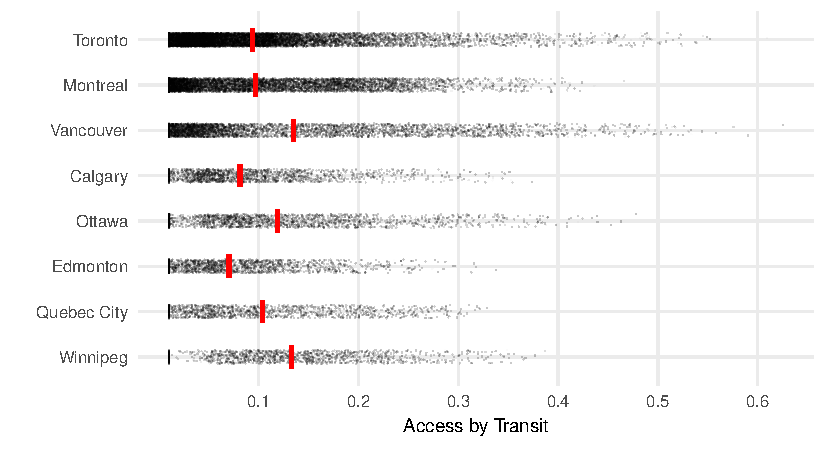
\includegraphics[width=5.5in]{figures/summary_plots/summary_AiT.pdf}}
	\vspace{2mm}
\end{figure}

\begin{figure}[H]
	\caption{Plot indicating the mean and distribution of access to jobs by car} 
	\label{sum_AiC}
	\centerline{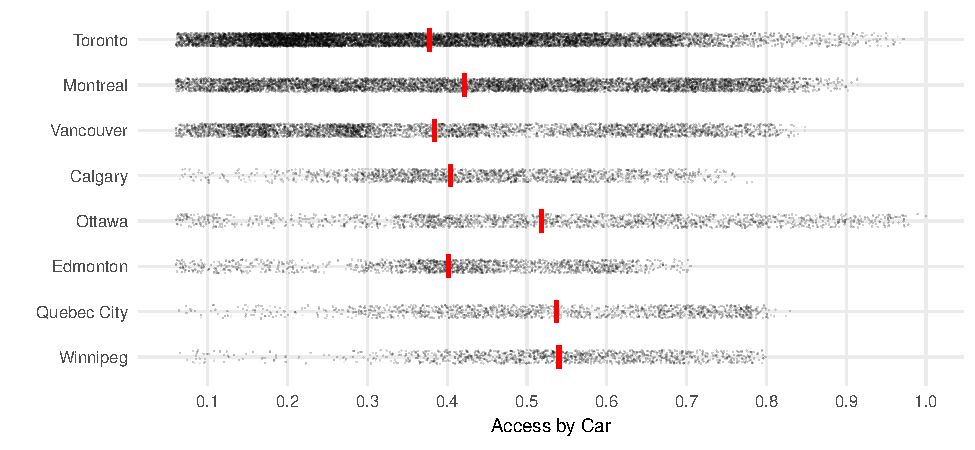
\includegraphics[width=6.5in]{figures/summary_plots/summary_AiC.pdf}}
	\vspace{0mm}
\end{figure}

% while central areas are Mtl and Tor, large employment areas in low density suburban business parks - with limited transit service. 

The maximum levels of transit access across the country are observed in central Vancouver and Toronto. Vancouver has a greater average than Toronto, meaning that Toronto has a greater abundance of suburban areas with low transit access, pulling down its regional average. Montreal is similar in size as Vancouver, but it has a lower mean and maximum level of access by transit. This can be explained by Montreal having less auto congestion \cite{tomtom2018}, and a greater network of private access highways, which expedite travel by car (i.e. car commuters can compete for more jobs). The mean level of auto access for Montreal is greater than Vancouver and Toronto. In the Montreal region, as well as Toronto, each municipality typically has its own transit agency, resulting in less fluid connections between regions, while the central transit agency in Vancouver services multiple municipalities (Vancouver, Richmond, Surrey, etc.)

Calgary and Edmonton have the lowest averages of access to jobs, both by transit and car. The urban form of these two cities is more dispersed, and there is greater separation between residential and employment areas. There is also a high concentration of employment in low-density suburban business parks which have limited transit service and require long walking times from bus stops to work destinations. The two Albertan cities also had the highest unemployment rates in 2016 compared to the other cities (the unemployment rate was 9.3\% in Calgary and 8.5\% in Edmonton), meaning that there are more people competing for jobs, bringing down the overall levels of access to jobs.

Winnipeg has the highest average level of access outside the three largest cities. Winnipeg has fewer periphery areas with limited transit service, meaning there are fewer areas pulling down its average. As well, from visual inspection, it has a greater spatial mix of jobs and housing. There is less concentration of employment in suburban business parks. Similar to Winnipeg, Ottawa and Quebec City a greater mix of jobs and housing than Calgary and Edmonton. However, Ottawa and Quebec City are each bisected by a large river with limited crossings, and different transit agencies operate on either side, limiting access to jobs on either side.




\subsection{Horizontal Equity}

Horizontal equity can be defined as how evenly a good or service is distributed amongst the overall population. We compute two measures to examine the horizontal equity of access to employment in Canadian cities. The first measure is the Coefficient of Variation (CV). The CV is a simple measure of relative variability, computed as the standard deviation divided by the mean. i.e.

\begin{equation}
CV_\lambda = |{\bar{A}_{p,\lambda}}|^{-1}\sqrt{\frac{\sum_{p=1}^{P}{(\bar{A}_{p,\lambda} - {A}_{p,\lambda}})^2}{n_p}} \hspace{1mm}
\end{equation}

Where $A_p$ is the accessibility index for person, $p$, in the population set of the region, $P$. $n_p$ is the total population. Each person, $p$, is assumed to have the accessibility of their home location, $i$. The Gini coefficient is a measure which has typically been used for analyzing income inequality. It has also recently been used to examine the horizontal equity of the supply of transit systems \cite{delbosc2011c,bertolaccini2013,welch2013}. Both \citeA{delbosc2011c} and \citeA{bertolaccini2013} used Gini coefficients to examine the equity of nearby transit availability, while \citeA{welch2013} used the Gini in measuring the inequality pertaining to different aspects of transit connectivity. We use the Gini to measure the inequalities of access to employment. The Gini is approximated as follows:

\begin{equation}
G_\lambda = \frac{\sum_{p=1}^{\lambda} \sum_{q=1}^{Q} | {A}_{p,\lambda} - A_{q,\lambda} |}{2 n_p \sum_{p=1}^{P} {A}_{p,\lambda}}
\end{equation}

Table \ref{gini} indicates the CV and Gini for each region. The greater the values, the greater amount of inequality of access to employment. The Gini, is based on differences in values, while the CV is on the squared differences in values, so the CV is more sensitive to those further from the mean. %The mean access of the region is also displayed for reference.

\begin{table}[H]
	\centering
	\vspace{4mm}
	\renewcommand{\arraystretch}{0.75} % Default value: 1
	\small
	\caption{CV and Gini coefficients of access to employment by mode}
	\vspace{2mm}
	\label{gini}
	\begin{tabular}{l|lll|lll}
		& \multicolumn{3}{c|}{Transit Access} & \multicolumn{3}{c}{Auto Access} \\
		\arrayrulecolor{lightgray}\cline{2-7}
		\arrayrulecolor{black}
		& Gini    & CV      & Mean    & Gini   & CV     & Mean  \\
		\hline
		Toronto     & 0.493 & 1.009 & 0.094 & 0.305 & 0.542 & 0.378 \\
		Montreal    & 0.499 & 0.922 & 0.097 & 0.317 & 0.551 & 0.422 \\
		Vancouver   & 0.510 & 0.968 & 0.135 & 0.317 & 0.560 & 0.384 \\
		Calgary     & 0.454 & 0.879 & 0.081 & 0.208 & 0.370 & 0.404 \\
		Ottawa      & 0.416 & 0.776 & 0.119 & 0.240 & 0.422 & 0.518 \\
		Edmonton    & 0.458 & 0.881 & 0.070 & 0.193 & 0.345 & 0.402 \\
		Quebec City & 0.416 & 0.749 & 0.104 & 0.174 & 0.303 & 0.537 \\
		Winnipeg    & 0.325 & 0.581 & 0.133 & 0.134 & 0.238 & 0.540 \\
		\hline
		All         & 0.489 & 0.959 & 0.101 & 0.289 & 0.506 & 0.411
	\end{tabular}
\end{table}

\newpage

Overall, there are higher values of inequality for Toronto, Montreal, and Vancouver. These regions also have some of the highest levels of access, which are typically located in their downtown cores, which are within walking distance to high employment areas, as well as rapid transit and regional transit services linking to other employment areas. The suburban areas of these regions are highly car dependent, and have limited transit service linking residential and employment zones. The range in access between the centre and periphery results in greater levels of inequality. Smaller cities tend to have more equal levels of access, but their central areas have lower levels of access than the centres of Toronto and Vancouver. Out of the mid-size cities, Edmonton and Calgary have greater levels of inequality of transit access, while Winnipeg has the least. 

It should be noted as well that the Gini will change depending on the scale of analysis \cite{bertolaccini2013}. For example, if we remove adjacent municipalities and only examine the City of Toronto, which has more frequent transit and transit-oriented development than adjacent municipalities, then the resulting Gini coefficient for transit access reduces from 0.493 to 0.327 as it includes fewer suburban areas with minimal transit service.

Figure \ref{lorenz} depicts the Lorenz curves for transit access to jobs and auto access to jobs in all eight cities combined. The two curves are in relation to the diagonal line of equality, the situation where the resource is distributed equally amongst the population (i.e. where everyone would have an equal level of access). The Gini coefficient is equivalent to the ratio of the area under the Lorenz curve divided by the area under the line of equality. The less of a gap between the curve and the line of equality, the less inequality within the region. Figure \ref{lorenz} further highlights how the distribution of transit access is more unequal than the distribution of auto access. For example, for auto access, 50\% (at x = 0.5) of the population has 30\% of total access in the region, while for transit access, 50\% of the population has less than 20\% of total access in the region.

\begin{figure}[H]
	\vspace{2mm}
	\caption{Lorenz Curve for access to jobs by transit and auto} 
	\label{lorenz}
	\centerline{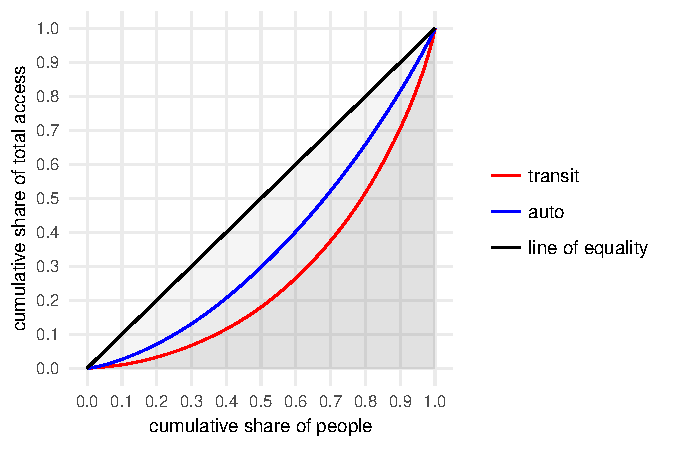
\includegraphics[width=4.5in]{figures/summary_plots/lorenz_all.pdf}}
	\vspace{2mm}
\end{figure}



\subsection{Transit Access \& Income Inequalities}

We then examine the vertical equity of transit access to jobs by analyzing its association with socioeconomic status (SES). For indicators of socio-economic status, we use four income-related categories from the census; unemployment rate (UR), the log of median after-tax household income ($\ln$ MHI), and two variables of low-income status tabulated by Statistics Canada, the low income cut-off (LICO) and the low income measure (LIM). The LIM is estimated as half the median of the adjusted household after-tax income, multiplied by the square root of household size. The LIM therefore accounts for how as a household has more members, its needs increase, but at a decreasing rate \cite{sc2016cdic}. Alternatively, the LICO pertains to households which are estimated to spend 20\% or more of their income on basic necessities (e.g. food, shelter, and clothing), relative to an average family. The LICO controls for household size and by region to account for differing costs of living. Each of these four income categories are all highly correlated. To examine their compounded effect, we also generate a combined measure of neighbourhood SES, weighting each of these four variables equally. This is generated as follows, where $\hat I$ pertains to the standardized score of each of the four measures.
\begin{equation}
I_\mu = 0.25 \hat I_{\ln MHI} - 0.25 \hat I_{UR} - 0.25 \hat I_{LIM} - 0.25 \hat I_{LICO}
\end{equation}
The lower the $I_\mu$, the lower the SES of the DA. 

We then generate Pearson correlation coefficients between these income variables and transit access to jobs. This is summarized in Table \ref{AiT_income} by each urban region.

\begin{table}[H]
	\vspace{2mm}
	\centering
	\renewcommand{\arraystretch}{0.75} % Default value: 1
	\caption{Correlation coefficient between transit access to jobs and income-related variables}
	\label{AiT_income}
	\begin{tabular}{l|rrrrr}
		& $\hat I_{LICO}$ & $\hat I_{LIM}$  & $\hat I_{UR}$ & $\hat I_{\ln MHI}$ & $\hat I_\mu$   \\
		\hline
		Toronto     & 0.43 & 0.32 & 0.04  & -0.29 & -0.32 \\
		Montreal    & 0.66 & 0.68 & 0.27  & -0.48 & -0.56 \\
		Vancouver   & 0.48 & 0.35 & 0.01  & -0.38 & -0.38 \\
		Calgary     & 0.45 & 0.38 & -0.01 & -0.36 & -0.32 \\
		Ottawa      & 0.53 & 0.43 & 0.20  & -0.38 & -0.44 \\
		Edmonton    & 0.58 & 0.46 & 0.09  & -0.53 & -0.48 \\
		Quebec City & 0.66 & 0.61 & 0.28  & -0.57 & -0.62 \\
		Winnipeg    & 0.59 & 0.58 & 0.28  & -0.64 & -0.59 \\
		\hline
		All         & 0.51 & 0.42 & 0.08  & -0.37 & -0.41
	\end{tabular}
\end{table}

Median household income, as well as the two low-income prevalence categories (LIM and LICO), are significantly correlated with transit access in each of the eight regions. This is the same overall relationship as in previous research in Toronto, which found that neighbourhoods of lower socioeconomic status tend to have better transit accessibility \cite{foth2013,elgeneidy2016tor}. Table \ref{AiT_income} indicates that this relationship is similar, and even accentuated, in the other seven cities. Comparing between cities, we observe that transit access in Toronto and Calgary have the weakest association with income categories, while Montreal, Winnipeg, and Quebec City have the strongest association. We also observe that unemployment is less associated with transit access compared with the other income categories. Toronto, Vancouver, and Calgary do not have a strong relationship between unemployment and transit access, while in the other cities, unemployed people are more likely to be in areas with good transit access.

We also examine the relationship with access to jobs, dis-aggregated by income level. Table \ref{AiT_income_u20} is the correlation of socio-economic levels with access only to low income jobs (under \$20,000 per year), and Table \ref{AiT_income_2040} is the correlation with access to low-to-medium income jobs (\$20,000 to \$40,000 per year). These results are very similar to the previous table looking at access to all job types.

\begin{table}[H]
	\vspace{2mm}
	\centering
	\renewcommand{\arraystretch}{0.75} % Default value: 1
	\caption{Correlation coefficient between income-related variables and transit access to low income jobs (under \$20,000 per year)}
	\label{AiT_income_u20}
	\begin{tabular}{l|rrrrr}
		& $\hat I_{LICO}$ & $\hat I_{LIM}$  & $\hat I_{UR}$ & $\hat I_{\ln MHI}$ & $\hat I_\mu$   \\
		\hline
		Toronto     & 0.41 & 0.33 & 0.05  & -0.33 & -0.33 \\
		Montreal    & 0.66 & 0.58 & 0.27  & -0.49 & -0.56 \\
		Vancouver   & 0.48 & 0.36 & 0.01  & -0.40 & -0.40 \\
		Calgary     & 0.43 & 0.35 & -0.02 & -0.34 & -0.29 \\
		Ottawa      & 0.52 & 0.42 & 0.20  & -0.37 & -0.43 \\
		Edmonton    & 0.58 & 0.46 & 0.09  & -0.53 & -0.48 \\
		Quebec City & 0.66 & 0.61 & 0.28  & -0.57 & -0.62 \\
		Winnipeg    & 0.58 & 0.56 & 0.27  & -0.63 & -0.58 \\
		\hline
		All         & 0.50 & 0.42 & 0.08  & -0.39 & -0.41
	\end{tabular}
\end{table}

\begin{table}[H]
	\vspace{2mm}
	\centering
	\renewcommand{\arraystretch}{0.75} % Default value: 1
	\caption{Correlation coefficient between income-related variables and transit access to low-to-medium income jobs (\$20,000 - \$40,000)}
	\label{AiT_income_2040}
	\begin{tabular}{l|rrrrr}
		& $\hat I_{LICO}$ & $\hat I_{LIM}$  & $\hat I_{UR}$ & $\hat I_{\ln MHI}$ & $\hat I_\mu$   \\
		\hline
		Toronto     & 0.44 & 0.35 & 0.06 & -0.33 & -0.35 \\
		Montreal    & 0.66 & 0.58 & 0.28 & -0.49 & -0.57 \\
		Vancouver   & 0.48 & 0.35 & 0.01 & -0.39 & -0.39 \\
		Calgary     & 0.46 & 0.38 & 0.00 & -0.37 & -0.32 \\
		Ottawa      & 0.53 & 0.43 & 0.20 & -0.38 & -0.44 \\
		Edmonton    & 0.58 & 0.46 & 0.10 & -0.54 & -0.49 \\
		Quebec City & 0.67 & 0.62 & 0.28 & -0.58 & -0.63 \\
		Winnipeg    & 0.59 & 0.58 & 0.29 & -0.65 & -0.60 \\
		\hline
		All         & 0.52 & 0.43 & 0.09 & -0.41 & -0.43
	\end{tabular}
\end{table}


Overall, from the results above, it can be concluded that transit access is vertically equitable, in each of these eight Canadian cities. Transit is serving low-income residents, those who theoretically have a greater need, more than high income residents. This could be due to a number of factors. One is that transit is being directly or indirectly planned to serve lower income residents. The location of low-income households is strongly correlated with population density, and transit is often planned to link concentrations of population and employment. Low-income housing is also usually planned in relatively denser, more centrally located areas, near transit, and typically away from wealthy suburban neighbourhoods. As well, centrally located areas with good transit access tend to have higher housing costs, and are likely to have more households willing to spend a greater percent of their income on housing, and less on private vehicles. Or people living near transit will be satisfied with relatively lower incomes as they will not have to bear the costs of paying for private vehicles. Finally, these results are also likely sensitive to the number affluent suburban neighbourhoods with poor transit access with relatively higher income levels. Many higher income residents typically give less value to transit when selecting housing, since they can afford a car, and place more value on larger dwelling and lot sizes in less dense neighbourhoods.




\subsection{Estimating the Extent of Transport Poverty}

Despite the overall positive outlook of the previous sets of analyses, there are still a number of low income or otherwise socially disadvantaged residents living in neighbourhoods with low transit access. For example, Figure \ref{AiT_Mu} shows the negative relationship between transit access to jobs and SES. However, there are still a number of a number of low-SES neighbourhoods with low access (dots in the bottom left of this plot). There could also be a number of low-SES households in neighbourhoods with higher levels of SES on average. This kind of place-based analysis shows the overall trends, but does not take into consideration the distributions of populations within each areal unit (e.g. within each dot in Figure \ref{AiT_Mu}).


\begin{figure}[H]
	\vspace{2mm}
	\caption{Scatter plot of transit access to jobs and the combined measure of socio-economic status ($I_\mu$)}
	\label{AiT_Mu}
	\centerline{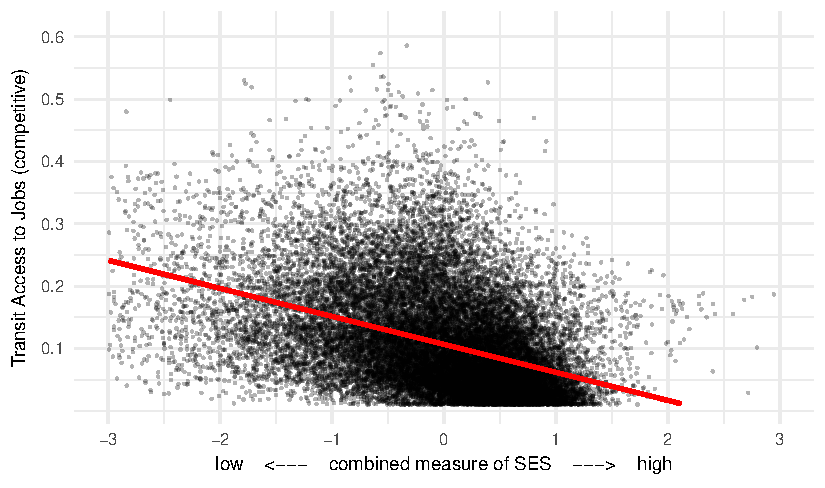
\includegraphics[width=5.5in]{figures/income_plots/AiT_Mmu.pdf}}
	\vspace{2mm}
\end{figure}

Households of low SES in areas of low transit access regions are at a greater risk of transport poverty, since they have limited transportation and financial resources to travel to, and participate in, activities such as employment \cite{preston2007,lucas2012}. Conducting analysis at a neighbourhood level potentially obfuscates these households if the neighbourhood has higher average levels of SES. 

Therefore, we tabulate the number of low-income populations in areas of low transit access. We first tabulate the number of low income residents living in the lowest deciles of transit access to jobs for each region. Tabulating by deciles provides a simple interpretation that X number of people living in the lowest 10\% of transit access for each region. However, this does not provide an adequate comparison between regions (there will always be a lowest 10\%). Accordingly, we tabulate populations under certain thresholds of transit access. Specifically, we count the populations in areas where transit access is less than 0.1 and where it is less than 0.05 (on the scale of competitive accessibility where 0 in the minimum and 1 is the maximum across observed for anyone across these eight Canadian regions). This allows for interpretation in the form of there are X number of people living in the areas of low transit access. 

These categories of low transit access are cross-tabulated with four socioeconomic variables in which are more likely to compound with low transit access and result in transport poverty. Firstly, we tabulate using two measures specified by Statistics Canada (2016), the low income cut-off (LICO) and the low income measure (LIM). The lower the income, the less likely they are to own a car, and more likely they will be reliant on public transit to access employment. The LICO accounts for regional variation in living costs, and therefore allows for more detailed comparison by region since costs of housing vary between as well as within cities (e.g. housing in downtown Vancouver or Toronto is generally more expensive than elsewhere). These households are less likely to be able to afford a vehicle for each working member of the household, and more likely to rely on transit \cite{seu2003}. If transit access is relatively low, it could increase the risk of transport poverty \cite{lucas2012}. As well, we sum cross-tabulations by two other measures of socio-economic status which could compound with transport disadvantage and result in transport poverty. One is recent immigrant status (immigrated between 2011 and 2016) as recent immigrants are more likely to rely on transit due to the time-intensive process of obtaining a driving license, the cost of a vehicle, and potential language barriers \cite{lo2011,farber2018}. Recent immigrants are also more likely to be in search of employment. Lastly we tabulate by the number of individuals who are unemployed, since previous research has linked difficulties of unemployed individuals in finding work with the inability to use a car and insufficient public transit options \cite{seu2003,merlin2017}. 

Table \ref{tab_decile} displays cross-tabulations of these SES variables with the lowest two deciles of transit access for each region. Similar to the results in the previous section, areas with low transit access tend to have relatively fewer numbers of people in low income households. However, we find that there are still nearly 150,000 people living low-income households according to the low income measure (LIM) who are in the lowest decile of transit access in their regions, and nearly 300,000 in the lowest quintile of transit access. Also, from our findings, recent immigrants tend to settle in more transit accessible areas, but there are still 45,000 recent immigrants living in the lowest decile of transit access and 107,000 in the lowest quintile of transit access. Looking at unemployment, there are 129,000 unemployed individuals living in the lowest quintile of transit access. 




\begin{table}[H]
	\vspace{2mm}
	\centering
	\renewcommand{\arraystretch}{0.75} % Default value: 1
	\caption{Counts of all low-income residents, unemployed, and recent immigrants (2011-2016) in the lowest decile and lowest quintile of transit access by region}
	\label{tab_decile}
	\begin{tabular}{ll|llll}
		& & LIM     & LICO    & Unem.   & Rec.Im. \\ \hline
		Toronto     & 10\%  & 60,260    & 34,775    & 25,320  & 20,805  \\
		& 20\%  & 130,915   & 85,965    & 53,340  & 50,160  \\
		& Total & 1,173,235 & 921,870   & 328,350 & 399,165 \\ \hline
		Montreal    & 10\%  & 26,860    & 14,050    & 11,790  & 2,300   \\
		& 20\%  & 50,945    & 29,345    & 22,725  & 5,895   \\
		& Total & 598,150   & 471,825   & 158,255 & 178,320 \\ \hline
		Vancouver   & 10\%  & 27,485    & 19,590    & 7,395   & 6,770   \\
		& 20\%  & 54,370    & 39,965    & 15,115  & 16,100  \\
		& Total & 422,365   & 349,300   & 85,505  & 147,790 \\ \hline
		Calgary     & 10\%  & 7,755     & 5,325     & 6,700   & 7,485   \\
		& 20\%  & 15,115    & 11,485    & 13,565  & 16,765  \\
		& Total & 118,005   & 108,445   & 73,835  & 91,935  \\ \hline
		Ottawa      & 10\%  & 8,440     & 4,120     & 3,365   & 875     \\
		& 20\%  & 15,150    & 9,230     & 6,860   & 3,415   \\
		& Total & 147,560   & 124,650   & 46,065  & 37,205  \\ \hline
		Edmonton    & 10\%  & 7,050     & 3,955     & 6,185   & 2,765   \\
		& 20\%  & 12,685    & 8,130     & 10,740  & 7,640   \\
		& Total & 112,125   & 99,295    & 58,750  & 76,920  \\ \hline
		Quebec City & 10\%  & 3,510     & 2,030     & 1,465   & 305     \\
		& 20\%  & 6,420     & 4,020     & 2,725   & 470     \\
		& Total & 74,500    & 61,545    & 18,095  & 12,890  \\ \hline
		Winnipg     & 10\%  & 5,965     & 4,890     & 1,910   & 3,935   \\
		& 20\%  & 10,475    & 8,465     & 3,915   & 6,610   \\
		& Total & 109,065   & 91,310    & 25,130  & 51,775  \\ \hline
		All         & 10\%  & 147,325   & 88,735    & 64,130  & 45,240  \\
		& 20\%  & 296,075   & 196,605   & 128,985 & 107,055 \\
		& Total & 2,755,005 & 2,228,240 & 793,985 & 996,000
	\end{tabular}
\end{table}
\newpage

% Table

\begin{table}[H]
	\vspace{2mm}
	\centering
	\renewcommand{\arraystretch}{0.75} % Default value: 1
	\caption{Counts of all low-income residents, unemployed, and recent immigrants (2011-2016) in areas of low (\textless 0.1) and extremely low (\textless 0.05) transit access}
	\label{tab_lowacc}
	\begin{tabular}{ll|llll}
	& $A_{i,T}$         & LIM            & LICO      & Unem      & Rec.Imm.         \\ \hline
	Toronto     & \textless 0.05 & 330,170   & 233,660   & 128,815  & 120,890 \\
	& \textless 0.1  & 637,670   & 471,715   & 212,395  & 224,890 \\
	& Total          & 1,173,235 & 921,870   & 328,350  & 399,165 \\ \hline
	Montreal    & \textless 0.05 & 136,070   & 87,360    & 52,990   & 22,700  \\
	& \textless 0.1  & 241,835   & 168,275   & 81,685   & 55,340  \\
	& Total          & 598,150   & 471,825   & 158,255  & 178,320 \\ \hline
	Vancouver   & \textless 0.05 & 115,165   & 85,525    & 30,400   & 39,220  \\
	& \textless 0.1  & 199,040   & 152,205   & 47,285   & 71,755  \\
	& Total          & 422,365   & 349,300   & 85,505   & 147,790 \\ \hline
	Calgary     & \textless 0.05 & 38,720    & 32,585    & 31,725   & 40,360  \\
	& \textless 0.1  & 74,150    & 65,510    & 53,160   & 66,330  \\
	& Total          & 118,005   & 108,445   & 73,835   & 91,935  \\ \hline
	Ottawa      & \textless 0.05 & 17,915    & 11,215    & 8,595    & 4,350   \\
	& \textless 0.1  & 44,520    & 32,110    & 20,415   & 13,130  \\
	& Total          & 147,560   & 124,650   & 46,065   & 37,205  \\ \hline
	Edmonton    & \textless 0.05 & 37,505    & 29,765    & 27,605   & 32,375  \\
	& \textless 0.1  & 69,035    & 57,825    & 42,880   & 52,890  \\
	& Total          & 112,200   & 99,360    & 58,770   & 76,955  \\ \hline
	Quebec City & \textless 0.05 & 9,620     & 6,395     & 4,250    & 1,075   \\
	& \textless 0.1  & 23,840    & 17,360    & 8,530    & 3,065   \\
	& Total          & 74,500    & 61,545    & 18,095   & 12,890  \\ \hline
	Winnipg     & \textless 0.05 & 6,735     & 5,525     & 2,230    & 4,385   \\
	& \textless 0.1  & 24,580    & 20,275    & 8,485    & 14,945  \\
	& Total          & 109,065   & 91,310    & 25,130   & 51,775  \\ \hline
	All         & \textless 0.05 & 691,900   & 492,030   & 286,610  & 265,355 \\
	& \textless 0.1  & 1,314,670 & 985,275   & 474,835  & 502,345 \\
	& Total          & 2,755,080 & 2,228,305 & 794,005  & 996,035
	\end{tabular}
\end{table}
\newpage

Table \ref{tab_lowacc} tabulates populations in areas that are low access ($A_{i,T} < 0.1$) and extremely low access ($A_{i,T} < 0.05$).  From this table, we observe that roughly half of these people of low SES live in areas of low access, and a quarter in areas with extremely low transit access. Calgary, Edmonton, and Toronto have particularly large counts relative to their totals, while more low SES people in Quebec City, Winnipeg, and Ottawa are living in areas with adequate transit access.

Research has also shown that available travel mode makes a substantial difference in terms of access to destinations, particularly the disparity between transit riders and those who have a private vehicle \shortcite{shen1998,benenson2011}. Some studies have found that low-income residents in central parts of cities are not disadvantaged by their relative spatial circumstance (central areas tend to have good access), but instead are disadvantaged by a modal mismatch \shortcite{blumenberg2004,grengs2010b}. We therefore tabulate by the number of people in low-SES categories who also live in areas where the ratio of transit access to auto access is less than 0.2 and less than 0.1. For these neighbourhoods, there is a chasmic gap in opportunity for individuals who are more likely to rely on transit compared to those who have a drivers license and regular access to a private vehicle. These cross tabulations are summarized in Table \ref{tab_ratio}. We observe that over 1 million of the 2.7 million urban Canadians living below the poverty line (LIM), are only afforded 1/5th or less the access by transit than access by car. As well, there are approximately 400,000 recent immigrants and 425,000 people who are unemployed that are under this threshold of the ratio transit access to auto access to jobs.

The web map and the maps in the appendix spatially show where low income households are located in each of these cities, overlaid onto a choropleth of transit accessibility, and thus indicates where people are at the greatest risk of being in transport poverty. 


\begin{table}[H]
	\vspace{2mm}
	\centering
	\renewcommand{\arraystretch}{0.75} % Default value: 1
	\caption{Count of all low-income residents, unemployed, and recent immigrants (2011-2016) in areas where the ratio of transit access to auto access is less than 0.2 and 0.1}
	\label{tab_ratio}
	\begin{tabular}{ll|llll}
			& $A_{i,T} / A_{i,D}$ & LIM     & LICO    & Unem.   & Rec.Im. \\ \hline
Toronto     & \textless 0.1  & 96,530    & 65,410    & 37,235  & 40,265  \\
& \textless 0.2   & 481,895   & 359,875   & 162,530 & 188,665 \\
& Total & 1,173,235 & 921,870   & 328,350 & 399,165 \\ \hline
Montreal    & \textless 0.1  & 51,650    & 36,360    & 24,165  & 9,260   \\
& \textless 0.2   & 224,770   & 159,240   & 78,040  & 55,530  \\
& Total & 598,150   & 471,825   & 158,255 & 178,320 \\ \hline
Vancouver   & \textless 0.1  & 20,335    & 15,585    & 5,625   & 6,410   \\
&\textless 0.2   & 107,675   & 84,305    & 29,210  & 41,065  \\
& Total & 422,365   & 349,300   & 85,505  & 147,790 \\ \hline
Calgary     & \textless 0.1  & 20,690    & 16,575    & 17,665  & 22,025  \\
& \textless 0.2   & 66,345    & 58,190    & 48,050  & 58,155  \\
& Total & 118,005   & 108,445   & 73,835  & 91,935  \\ \hline
Ottawa      & \textless 0.1  & 7,975     & 5,035     & 3,665   & 2,210   \\
& \textless 0.2   & 48,840    & 36,245    & 21,090  & 14,270  \\
& Total & 147,560   & 124,650   & 46,065  & 37,205  \\ \hline
Edmonton    & \textless 0.1  & 23,535    & 18,180    & 18,290  & 18,000  \\
& \textless 0.2   & 68,725    & 57,595    & 42,635  & 51,465  \\
& Total & 112,200   & 99,360    & 58,770  & 76,955  \\ \hline
Quebec City & \textless 0.1 & 8,645     & 5,805     & 3,585   & 865     \\
& \textless 0.2   & 26,750    & 19,710    & 9,180   & 4,300   \\
& Total & 74,500    & 61,545    & 18,095  & 12,890  \\ \hline
Winnipg     & \textless 0.1  & 5,335     & 4,410     & 1,610   & 3,665   \\
& \textless 0.2   & 23,260    & 19,160    & 8,265   & 14,780  \\
& Total & 109,065   & 91,310    & 25,130  & 51,775  \\ \hline
All         & \textless 0.1  & 234,695   & 167,360   & 111,840 & 102,700 \\
& \textless 0.2   & 1,048,260 & 794,320   & 399,000 & 428,230 \\
& Total & 2,755,080 & 2,228,305 & 794,005 & 996,035
	\end{tabular}
\end{table}
\newpage





\subsection{Characteristics of Areas Vulnerable to Transport Poverty}

The previous tables indicate that there are a substantive number of Canadians of low socioeconomic status living in areas of low transit access. In this section, we analyze characteristics of areas that have high levels of being at risk of transport poverty, for descriptive purposes as well as to support discussion and policy recommendations in the subsequent section. 

From visual inspection of the web map and the maps included in the Appendix, the areas with the lowest levels of transit access to employment typically occur in more peripheral areas. This is expected since peripheral locations are typically further from employment centres and are more likely to be adjacent to rural areas with less employment opportunities. Those peripheral areas that do have adequate transit access tend to be either located on major travel corridors with relatively frequent local transit service, near stops of regional rail and bus lines, or are quite proximate to employment areas (e.g. within a reasonable walking distance). 

Within low transit access areas, there are visible spatial clusters of residents who are more likely to be reliant on transit (e.g. low-income, unemployed, and recent immigrants). To examine the characteristics of these areas in more detail, we first need to classify Dissemination Areas (DA) in terms of their risk of experiencing transport poverty. Theoretically, transport poverty is more likely to occur where there is low transit access and lower levels of SES \cite{preston2007,lucas2012}. Ideally, this would be parameterized as models where the independent variables are measures of activity participation and the dependent variables are various measures of transport (dis)advantage, demographics, and socioeconomic status, as well as inclusion of any random effects. Creating such a model would require comprehensive travel survey data (which is lacking Canada wide) and rigorous work on how to explicitly define and generalize dependent and independent variables to areal units. For the scope of this thesis, this is simplified to assume that areas at risk of transport poverty are those with low transit access to employment, and high number of people living in low-income households. We use the compounding effect of these two variables to classify DAs into four categories of risk of transport poverty (low, moderate, high, and very high). This relationship is visualized in Figure \ref{plane_risk}, where each dot represents a DA. The percent of DAs in each classification for each region is displayed in Table \ref{pov_by_city}.

\begin{figure}[H]
	\vspace{4mm}
	\caption{Classifying DAs in terms of risk of experiencing transport poverty} 
	\label{plane_risk}
	\centerline{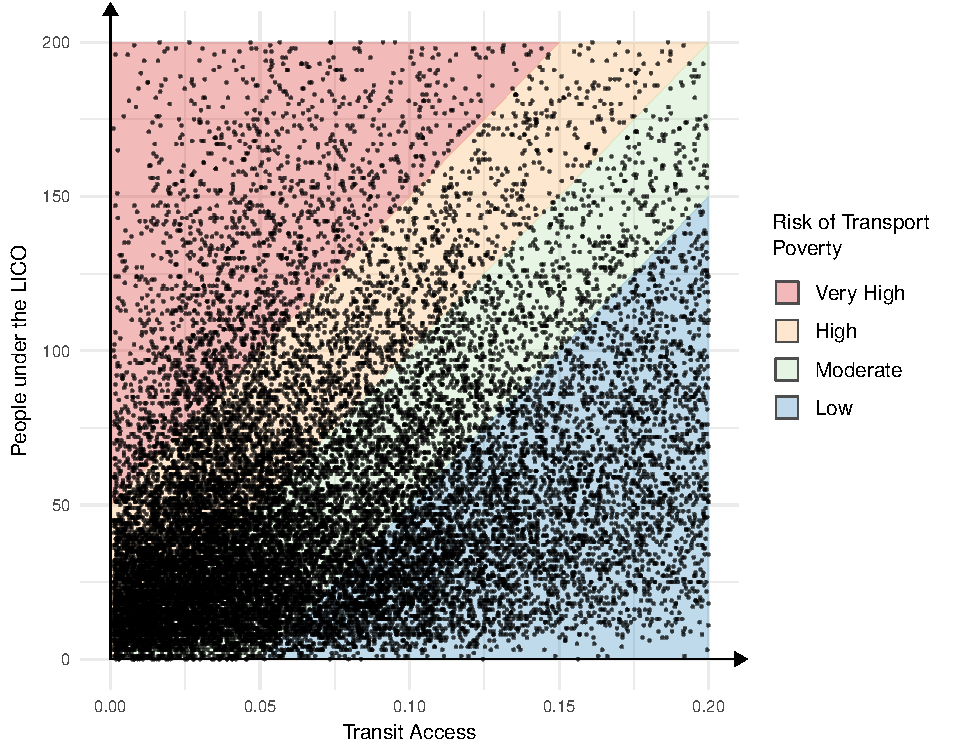
\includegraphics[width=6.5in]{figures/built_env/plane_risk.pdf}}
	\vspace{2mm}
\end{figure}

\begin{table}[H]
	\vspace{2mm}
	\centering
	\renewcommand{\arraystretch}{0.75} % Default value: 1
	\caption{Percent of DAs classified by risk of experiencing transport poverty in each region}
	\label{pov_by_city}
	\begin{tabular}{l|llll}

		& Low      & Moderate   & High     & Very High  \\
		\hline
		Toronto     & 30.0\%   & 31.0\%     & 24.0\%   & 15.1\%     \\
		Montreal    & 30.5\%   & 32.1\%     & 26.9\%   & 10.5\%     \\
		Vancouver   & 35.9\%   & 20.7\%     & 27.7\%   & 15.8\%     \\
		Calgary     & 35.6\%   & 34.3\%     & 19.9\%   & 10.2\%     \\
		Ottawa      & 53.6\%   & 24.2\%     & 13.5\%   & 8.7\%      \\
		Edmonton    & 29.9\%   & 35.0\%     & 24.0\%   & 11.1\%     \\
		Quebec City & 49.6\%   & 34.4\%     & 13.8\%   & 2.1\%      \\
		Winnipeg    & 62.4\%   & 22.0\%     & 8.9\%    & 6.7\%      \\
		\hline
		All         & 34.8\%   & 29.6\%     & 23.2\%   & 12.4\%    
	\end{tabular}
\end{table}

The cities of Toronto and Vancouver have the greatest percent of their DAs that have a high risk of transport poverty, and the smaller cities of Winnipeg and Quebec City have the lowest. Toronto and Vancouver are also the two cities which have been reported on the most in terms of experiencing rising housing costs and sub-urbanization of poverty \cite{ades2012,ades2016poverty}. The results in Table \ref{pov_by_city} are also aligned with the findings in Section 5.3 of comparing transit access and income inequalities.

To examine the characteristics of these areas in more detail, we plot summaries of three built environment measures; population density, period of housing construction, and structural type of dwelling. Figure \ref{built_popdense} shows the distributions of population density for the four categorizations of transport poverty. Areas with the lowest risk of transport poverty have the highest percent of population living in areas with high population density, and by far the lowest percent in areas with low population density. This is expected since central areas are generally more dense and that transit is generally planned to serve areas with greater levels of population. Notable in this plot is that areas of very high risk of transport poverty tend to have higher levels of population density than those at high or moderate risk. 

\begin{figure}[H]
	\vspace{4mm}
	\caption{Plot of population density in DAs classified by risk of transport poverty} 
	\label{built_popdense}
	\centerline{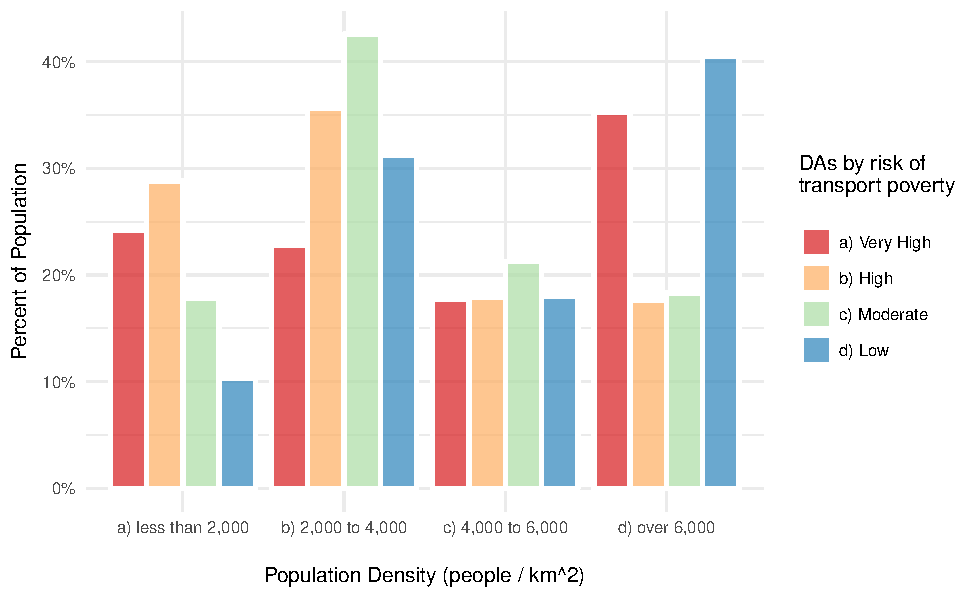
\includegraphics[width=6.5in]{figures/built_env/built_popdense.pdf}}
	\vspace{2mm}
\end{figure}

To examine further, we plot by the percent of dwellings units in each category by their structural type (Figure \ref{built_type}). This is aggregated into four categories; single-detached homes, attached homes and duplexes, apartments with fewer than five stories, and apartments with five stories or more. We see that areas with a very high risk of transport poverty are more likely to have tall apartments, while areas with moderate or high risk tend to be composed of detached single-family homes. Areas with low risk of transport poverty are more diverse in terms of their dwelling type. 

\begin{figure}[H]
	\vspace{4mm}
	\caption{Plot of dwelling type in areas with low transit access and areas at risk of transport poverty} 
	\label{built_type}
	\centerline{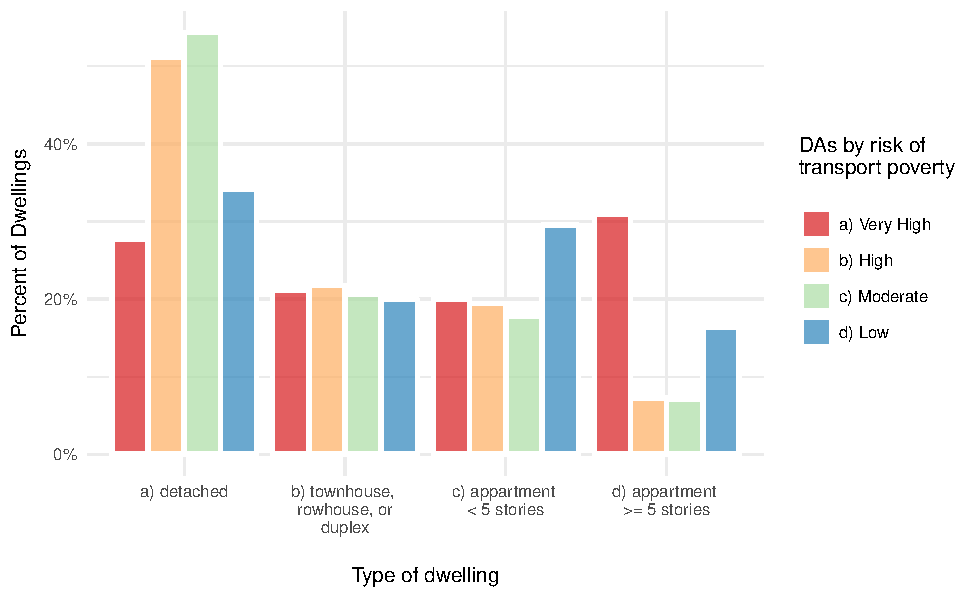
\includegraphics[width=6.5in]{figures/built_env/built_type.pdf}}
	\vspace{2mm}
\end{figure}

As well, we also plot the percent of dwellings by their period of construction (Figure \ref{built_period}). We see that areas with more recent housing, the greater the risk of transport poverty. This is expected since older parts of cities are more centrally located and tend to have higher employment densities. As well, unlike other services (e.g. paved roads, running water, etc.), it is not usually a strict municipal requirement for transit to be provided at the onset of new residential development. Therefore, some areas with high risks of transport poverty could be places where transit provision has failed to keep up to the demand of new residential development.

\begin{figure}[H]
	\caption{Plot of dwelling period of construction in DAs classified by risk of transport poverty} 
	\label{built_period}
	\centerline{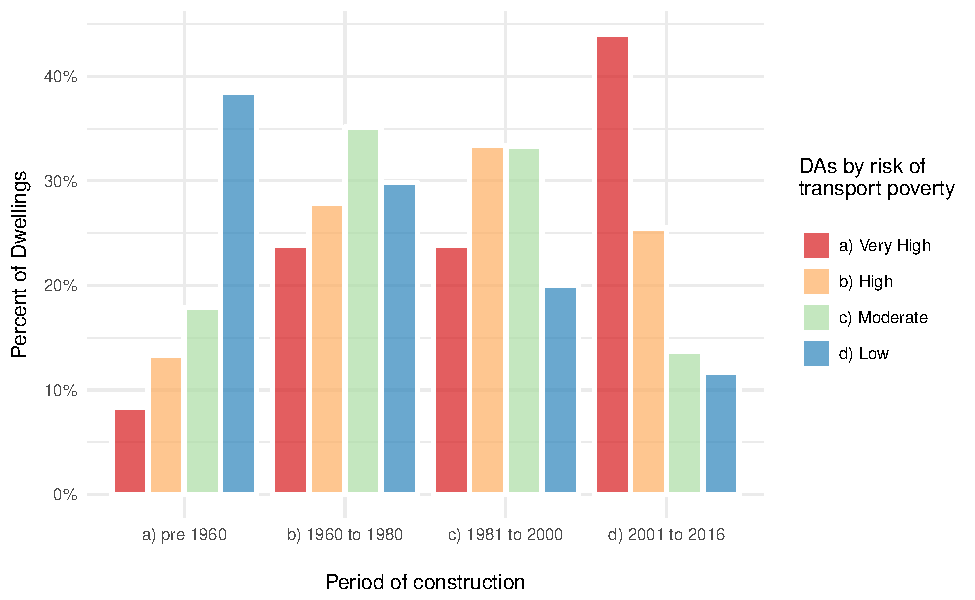
\includegraphics[width=6.5in]{figures/built_env/built_period.pdf}}
	\vspace{2mm}
\end{figure}

The more recent the development, the more likely it is to have a greater percent of residents who have moved there recently. Figure \ref{built_move} shows that over 50\% of people living in areas with very high risk of transport poverty had moved there sometime between 2011 and 2016. This includes a greater percent of people moving from within the same CSD (i.e. within the same municipality), from a different CSD, and from outside Canada (i.e. recent immigrants). This supports theories on suburbanization of poverty given that high risk areas have higher concentrations of poverty, recent mobility, and include more high rise apartments which typically have lower housing costs than single family homes.

\begin{figure}[H]
	\caption{Plot of mobility status in DAs classified by risk of transport poverty} 
	\label{built_move}
	\centerline{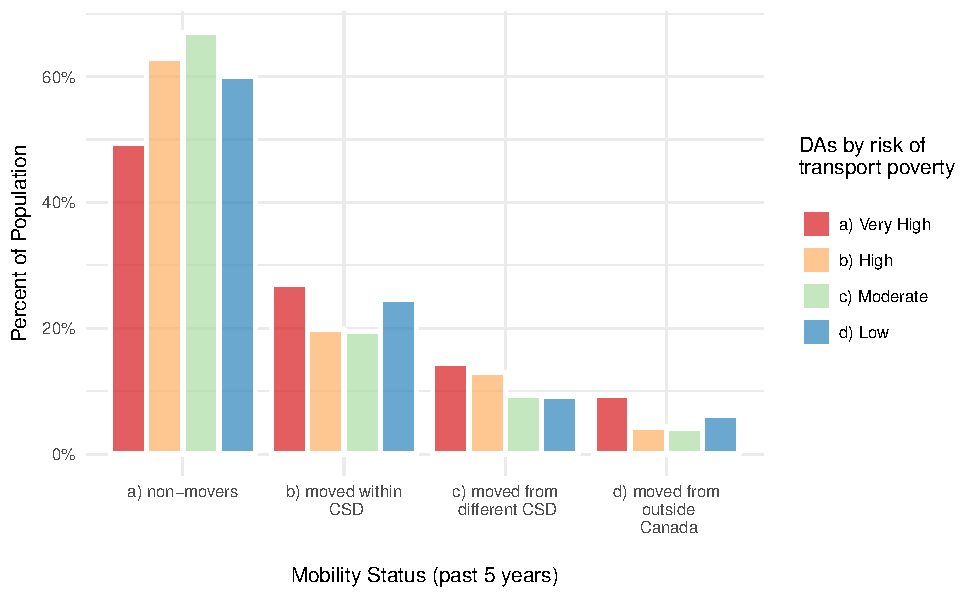
\includegraphics[width=6.5in]{figures/built_env/built_mobility.pdf}}
	\vspace{2mm}
\end{figure}

From the above plots, we can summarize that areas at the highest risk of transport poverty are more likely to be built within the 21st century, have a greater percent of apartment buildings, and are more dense than prototypical suburban neighbourhoods of low transit access. As well, people within these areas are more likely to have moved there recently (2011 to 2016). Areas of moderate to high risk are more likely to be typical single-detached suburban homes.

For more in depth analysis, we conduct a $k$-means cluster analysis of zones at risk of transport poverty in order to generate a typology that can be used for policy recommendations. $k$-means clustering seeks to minimize the Euclidean distance in an n-dimensional space between the attributes of variables and the means of clusters ($k$ is the specified number of clusters). Specifically we cluster on DAs that we classified as high or very high risk of transport poverty. We cluster these DAs using five relevant variables; access to jobs by transit, access to jobs by car, population density, percent of population living in apartments, and number of residents in low-income households. The resulting number of clusters ($k = 2$) were was determined via by generating a Scree plotting plot (a plot of the total within-clusters sum of squares versus versus the number of clusters, $k$) and then selecting the $k$ where the graph provides the greatest change in slope (see Figure \ref{scree_plot}). The means of the variables selected in the cluster analysis for the two resulting groups are displayed in Table \ref{t_cluster}. Table \ref{t_cluster} also shows the number of DAs in each category, as well as the number of DAs that were previously categorized as being high or very high risk of transport poverty. There is a greater proportion of DAs that have a very high risk of transport poverty (very high levels of low income and low transit) in the first group, which also has greater population density and percent of people living in apartments.

\begin{table}[H]
	\vspace{4mm}
	\centering
	\renewcommand{\arraystretch}{0.75} % Default value: 1
	\caption{Cluster analysis results of DAs at risk of transport poverty}
	\label{t_cluster}
	\begin{tabular}{l|ll}
		mean & Group A & Group B \\ \hline

		Auto Access               & 0.497   & 0.236   \\
		Transit Access                  & 0.122   & 0.032   \\
		Population Density (ppl/km2)          & 8,670    & 3,335    \\
		People under the LICO        & 267     & 76      \\
		Percent living in apartments & 75\%    & 16\%   \\ \hline
				n DAs                         & 2,071    & 7,420  \\
				n Very high risk of transport poverty &  1,288 & 1,850 \\
				n High risk of transport poverty & 783 & 5,570 
	\end{tabular}
\end{table}

\begin{figure}[H]
	\vspace{1mm}
	\caption{Scree plot for determining the number of clusters, $k$} 
	\label{scree_plot}
	\centerline{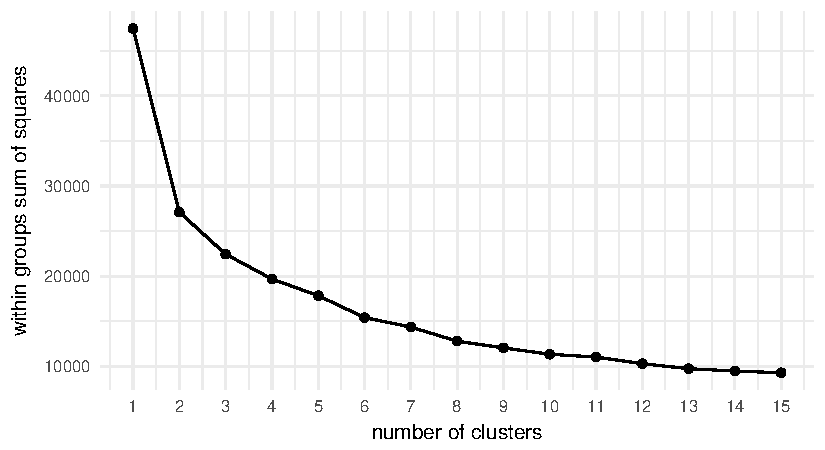
\includegraphics[width=5.5in]{figures/built_env/scree_plot.pdf}}
	\vspace{2mm}
\end{figure}

We can summarize by saying that there are two main typologies of areas in which people are at high risk of experiencing transport poverty. One are areas with high density, primarily apartments, with very high concentrations of low income residents, and moderate levels of transit access to employment (Group A). The second (Group B) are more peripheral, typical suburban single family housing, low density neighbourhoods, with extremely low levels of transit access, and wider gap between the relative level of transit access to auto access, but have fewer low income residents. Figure \ref{C_van_main} shows the spatial pattern of these two clusters for Vancouver. The majority of the central part of the region does not have either group. DAs in Group A are located more within the "inner-suburbs" in higher density areas with some transit service, but with high concentrations of poverty. DAs in Group B are primarily suburban areas with very poor transit provision. Similar patterns are visible in other cities (see the maps in the Appendix).

\begin{figure}[H]
	\caption{Map of the location of cluster groups for Vancouver} 
	\label{C_van_main}
	\centerline{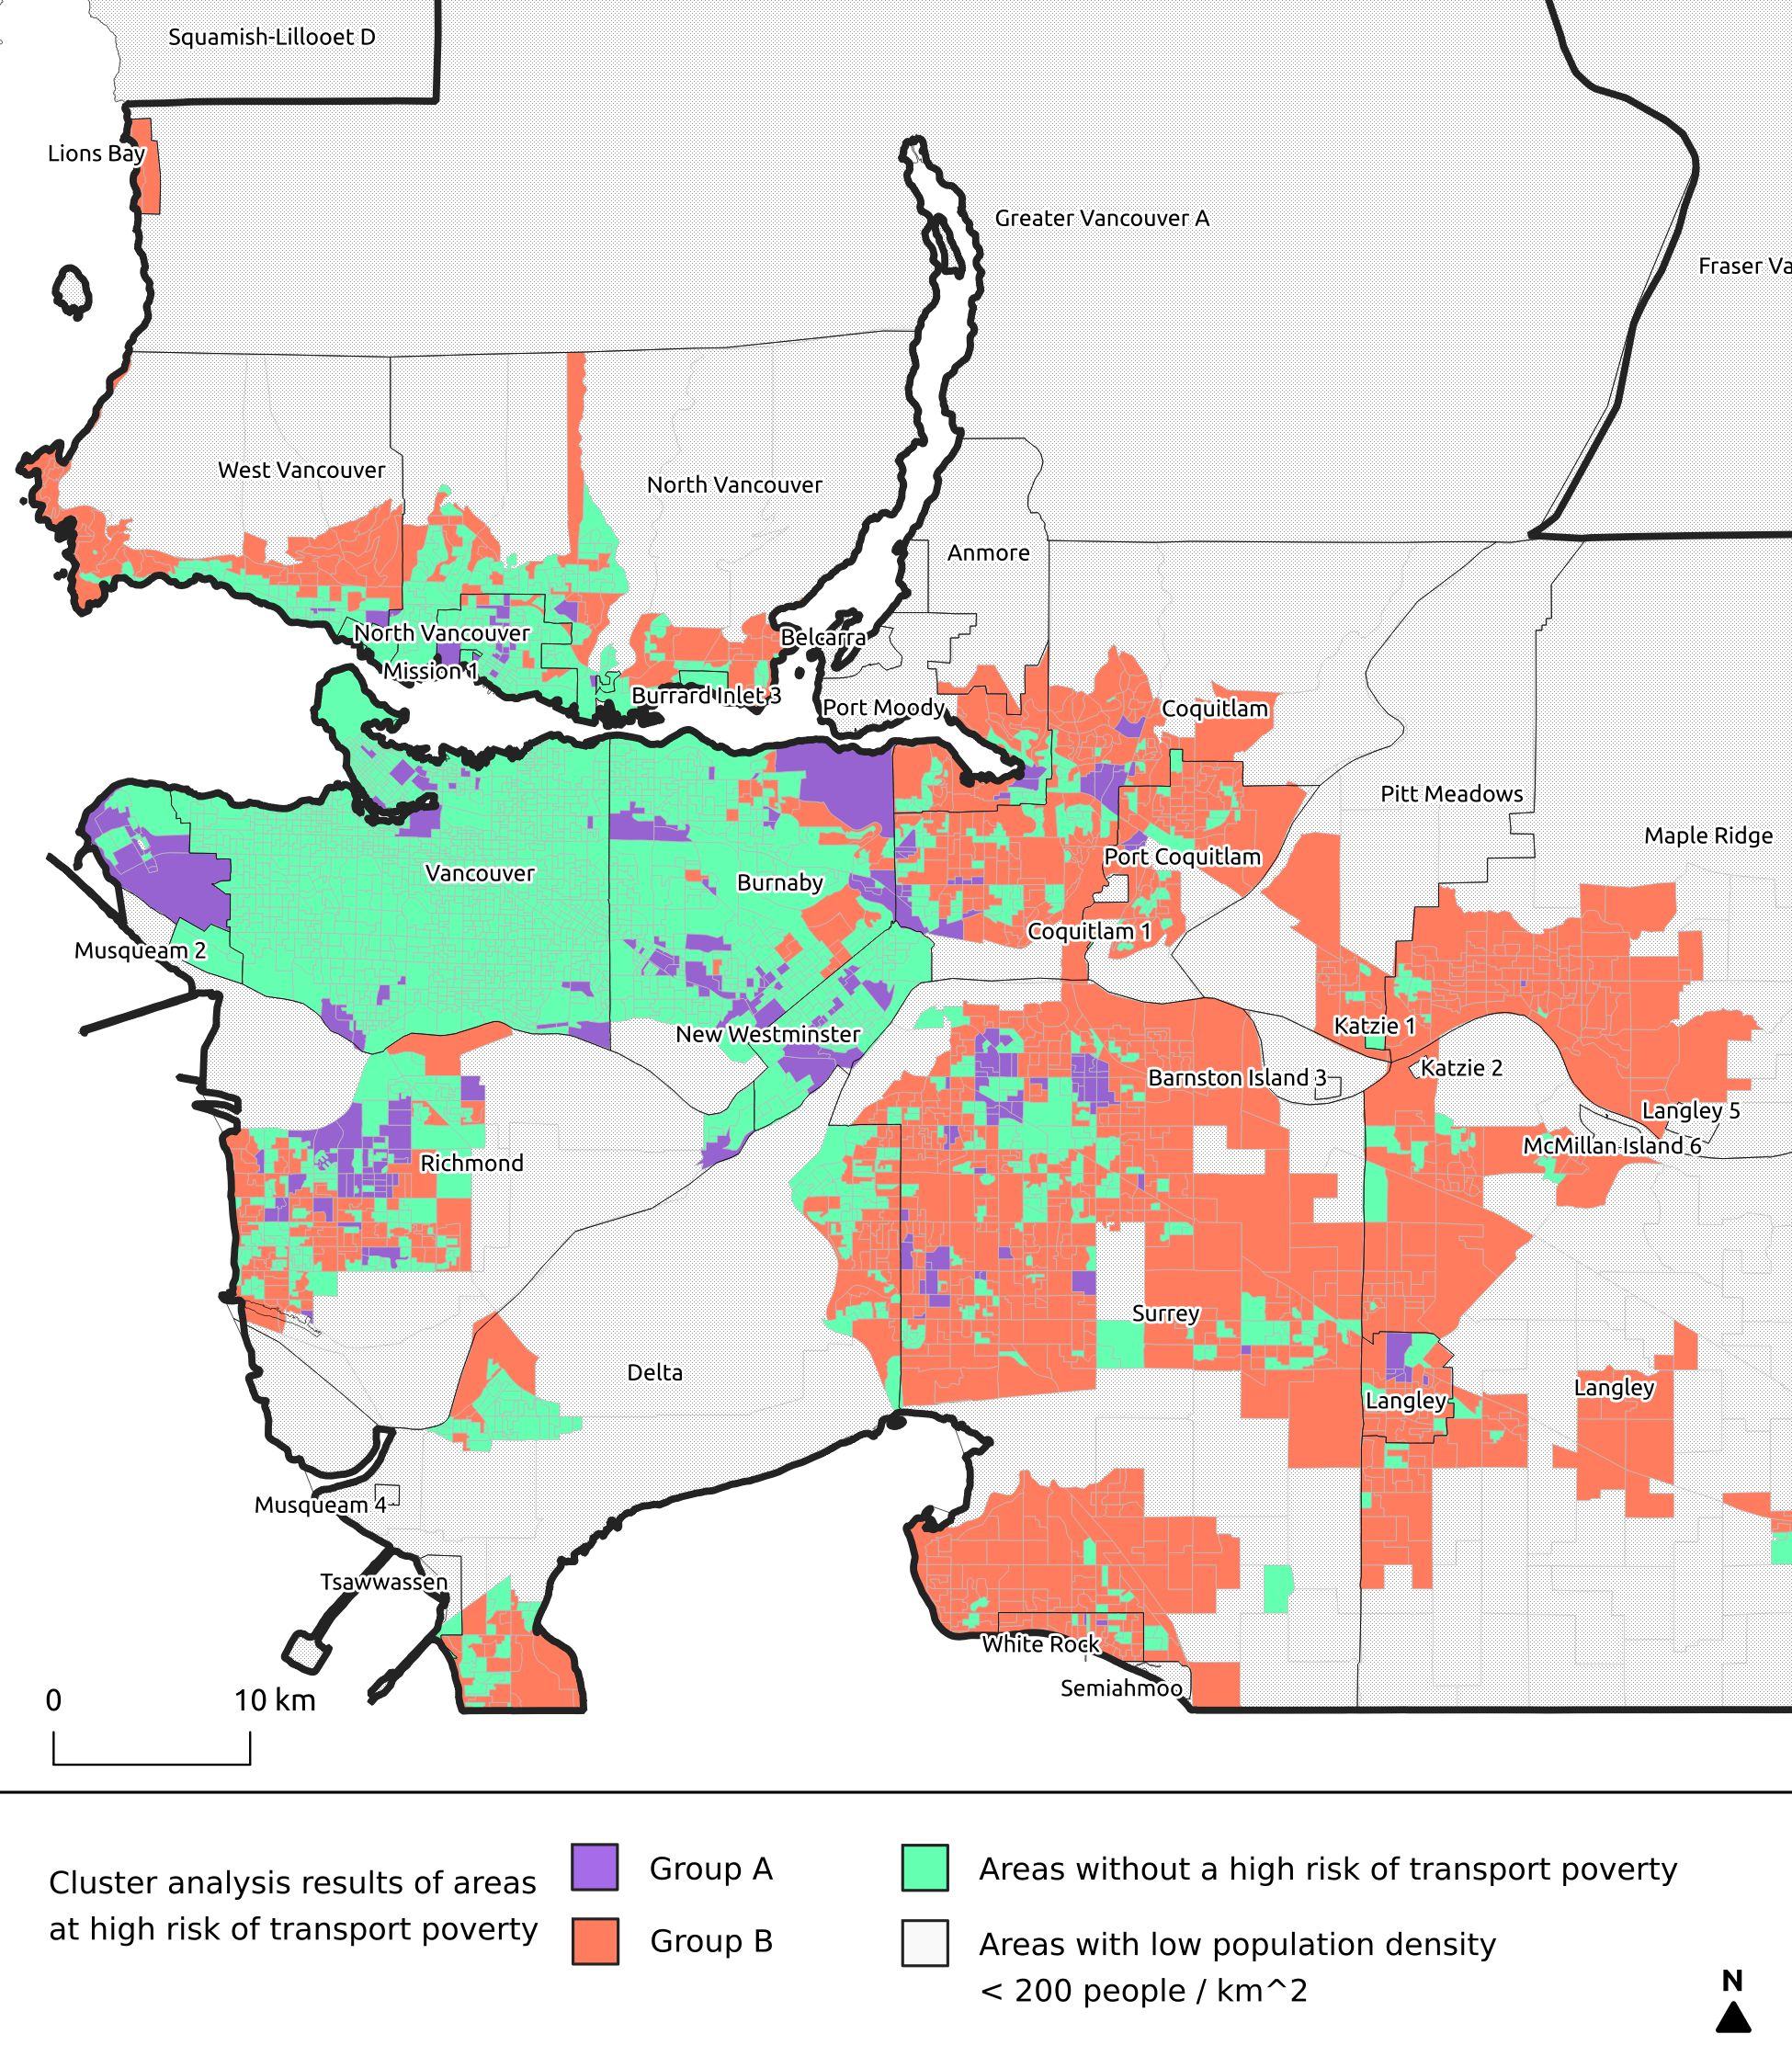
\includegraphics[width=6.5in]{figures/cluster_maps/C_van}}
	\vspace{2mm}
\end{figure}



\newpage

\section{Policy Recommendations}

The research in the previous sections show that while there are not widespread systemic vertical inequalities in transit access, there are still a substantial number of low-income Canadians living in areas of low transit access. The compounding effects of low transit access and low SES increase the risks of transport poverty, potentially limiting people in their ability to travel to and participate in daily activities, including finding and retaining employment \cite{preston2007,lucas2012}

Because of spatial and temporal variations in land use and urban form, completely equitable transport service, and equal access to destinations in particular, is not possible. Even if it was, an equality of outcome should not be the objective. People will inherently have different preferences and values in terms of where they choose to live in reference to accessible destinations and urban form more generally. However, a common goal of transport policy and planning is to reduce vulnerability to transport poverty and minimize wide-ranging inequalities of access, as well as increase the overall accessibility of a region \cite{seu2003,martens2012justice,martens2016,pereira2017}, i.e. to make transport more equitable, both horizontally and vertically. Literature in transportation planning has argued that transport networks should not be insufficient to deter people in their ability to travel to key destinations and participate in activities pertinent to their well-being \cite{preston2007,lucas2012,martens2016}. Investing in public transport to improve accessibility, particularly focused towards those at risk of transport poverty, has the potential to reduce inequalities, limit barriers to activity participation, and foster social and economic inclusion. 

This theoretical background combined with the empirical research in this thesis in Canada leads to the broad conclusion that transport policy in Canadian cities should focus towards improving transit service to low access neighbourhoods, with particular focus towards those neighbourhoods with more low-income households since they are more likely to be reliant on transit. This would help alleviate risks of transport poverty and reduce inequalities of transit access. As well, our research (see section 4.5), along with other papers \cite{owen2015,boisjoly2016}, indicate a strong correlation between transit access and transit mode share. So improving transit access in areas with a greater number of low-income households would not only help alleviate the risks of transport poverty, but it will most likely increase transit mode share for the overall population, which would have a number of environmental and economic benefits. 

Unfortunately, there is only a limited amount funds and resources available for improving urban transportation in Canadian cities. Certainly, this points towards advocating for increasing public funding for public transit service, either through raising taxes (e.g. like gas taxes or congestion charges) or re-allocation of government spending on other infrastructure (e.g. shift spending on highways to spending on transit). However, it would be quixotic to think that there will be a sufficient amount of funds for desirable levels of public transit provision in urban areas across Canada in the near future. The prevailing challenge of urban transportation planning is deciding how to allocate scarce funds and resources to where they are to be the most effective, and to avoid investments which are unlikely to generate results. Resources should be allocated not only to where they will be most cost effective in improving ridership, mobility, and accessibility, but also in where they have the greatest potential in alleviating transport poverty.

The previous section indicates that there are two types of areas at risk of transport poverty. The first group have high levels of population density (e.g in apartment towers) and high concentration of low income residents. These are usually located in the "inner-suburbs" of urban areas, and typically already has some transit service in place, but the existing service does not come close to meeting the need of residents. Due to greater density, improving transit access in these areas would be the most effective in reducing risks of transport poverty for a large group of people. Indeed, those areas with particularly high concentrations would be ideal candidates for new rapid or regional transit stations. However, this would only be realistic solution in a few locations given the high capital costs of such infrastructure. For most areas, more cost effective solutions should be considered for upgrading existing service. One would be increased frequency on existing routes by adding more vehicles to limit wait times, particularly for routes with large headways. Travel times could also be reduced by implementing express lines which make fewer intermittent stops (either by removing stops on existing lines or adding express buses, depending on the situation). Another cost-effective solution would be to alter the design of roads to incorporate dedicated bus lanes (i.e. BRT), to depose delay caused by auto congestion. The majority of suburban arterial roads have ample room to implement dedicated bus lanes, a convenience of the unbridled auto-oriented planning of the previous decades. The main barrier would be to convince the public to remove a lane of traffic.

Improving transit access in lower density, single-family housing areas is a greater challenge given the greater disbursement of individuals. In these regions, many transit agencies opt for coverage rather than directness in their design of suburban transit routes. It may be possible that faster, more direct, routes in some instances will have a greater potential in providing greater access, depending on the spatial distribution of transit need in the region \cite{walker2012}. Similarly, transit networks should focus on providing better links to suburban employment locations, many of which currently have sparse transit service. Major transit lines in Canadian cities tend to have a radial pattern, but there should be more linkages between more peripheral residential and employment areas given the growth of suburban employment centres and suburb-to-suburb commuting patterns \cite{blais2015}. Analysis on re-configuring routes and networks to improve access, however, would require more detailed case-based studies of accessibility gains or losses from different re-configuration scenarios and assessing which would derive the most benefit.

Another potential solution, or as an augmentation to other solutions, is to provide subsidies for ride-sharing or implement demand responsive transit service. This could be beneficial in less-populated suburban areas, where implementing traditional transit service has substantial monetary costs, or in areas where there is a last mile problem. A few regions have begun to experiment with this type of service. For example, the growing town of Innisfil (north of Toronto), recently partnered with Uber to subsidize an on-demand ride-sharing service, as a more economical alternative to developing traditional, fixed-route, transit service \cite{innisfil2017}. While this may be a solution for alleviating transport poverty in areas with less demand (e.g. like Innisfil), it may not be applicable in urban areas where there is already heavy congestion or a greater need for adding more higher capacity transit \cite{mageean2003}. Evaluating the success of such projects however will provide useful knowledge on how and where demand responsive transit could be implemented elsewhere in Canada, and whether it can be appropriately scaled if demand for transit increases.
It should be noted that some other studies, in aims to reduce transport poverty in low density conditions, have recommended implementing policies aimed at helping those without a private vehicle to gain access to them in order to improve their level of access \shortcite{shen1998,lucas2003,blumenberg2004}. However, the scale and scope of providing families with cars has many uncertainties at a regional scale, and doing so may expedite problems of congestion, emissions, and parking capacity. Subsidizing ride-sharing or providing demand responsive transit would likely be more cost efficient and less problematic.

In conjunction to the aforementioned recommendations for transit improvement, municipalities and regional planners should also enforce land use policies which restrict urban sprawl and zone for urban intensification and mixed-use development, in order to help reduce commute times and auto-dependency. This should include planning any future development of housing for low-income residents and recent immigrants to be in areas with high transit access. This should also include focusing some employment growth in areas which have existing transit service, but have low accessibility metrics due to a local absence of jobs - areas where there are an abundance of labourers who currently have to travel further to find employment. These ideas of "smart growth" and denser, transit-oriented development, are often cited by urban planners to reduce congestion and environmental impacts \cite{bernick1997}. This sphere of development strategies can also reduce risks of transport poverty by providing more nearby opportunities, and reduce the gap between transit and auto access. However, there is currently tension between developers, planners, and government officials over policies pertaining to future development strategies. For example, the Ontario government developed a plan to limit urban sprawl by delineating a protective greenbelt around the Toronto region, yet concurrently, the same government continues to build peripheral motorways which perpetuate and encourage suburban growth \cite{macdonald2012}. 

As well, despite the existing goals of transit-oriented development and other smart-growth strategies, Figure \ref{built_period} indicates that newly developed areas are still more likely to be at a higher risk of transport poverty. This is likely due to transport planning being several years behind the construction of new developments in terms of providing access to destinations. Arguably, transit should be treated as an essential service, in that development should not occur until there is a certain level transit provision, similar to how residential development is required to support municipal services like new roads, sewers, and stormwater management.

Lastly, it is possible that in the long term, providing better transit access to a neighbourhood, and well designed transit-oriented development more generally, could increase demand and costs for housing. This would likely first affect low-income people in these areas for whom transit is the only alternative for daily travel. Rising costs could then result in displacement to less accessible areas. This indicates the importance of policy directed towards maintaining stability and affordability of housing costs, in order to break any cycles of urban displacement. This also shows the importance of insuring for minimum standards of accessibility across an entire region, given other uncertainties of housing markets and living costs in the near future.




\newpage

\section{Conclusion}

In this study, we computed comparative measures of access to employment by transit for Canada's eight largest urban regions. Specifically, we computed a measure which is comparable between cities by accounting for competition among both the labour force and employers, time fluctuations in transit schedules, and unequal counts of jobs and workers in each region. We find that at a regional level Vancouver and Winnipeg have the highest average levels of access, and Calgary and Edmonton have the lowest. The neighbourhoods with the maximum level of access are in central Toronto and Vancouver.

We used these measures to examine the equity of transit access to jobs within these regions. Using Gini coefficients to examine horizontal equity, we found that transit provision is more equally distributed in the smaller cities like Winnipeg and Quebec City, while larger urban areas like Toronto, Montreal, and Vancouver have a greater overall inequality of transit access to jobs. Access by transit is also more unequally distributed than access by car. In examining vertical equity, we find that low-income households, on average, have higher values of transit access to employment than the overall population. These trends are similar when comparing between all eight cities. Despite an overall positive outlook, there are still many households at risk of experiencing transport poverty. We estimate that 200,000 low income individuals are in the lowest quintile of transit access, and 800,000 have less than 1/5th the access by transit than by car. Furthermore, there are approximately 110,000 recent immigrants and 125,000 unemployed individuals who live in the lowest quintile of transit access. 

Recommendations to reduce inequalities in transit access and limit risks of transport poverty include focusing future transit investments in areas which have high concentrations of low-income households and low levels of transit access, upgrading bus service to have dedicated lanes, offer more direct or express services, intensification and diversity of land-use to increase accessibility and reduce commute distances, as well as a consideration of subsidizing ride-sharing or implementing demand-responsive transit in areas of low density. Doing so would help reduce the risks of transport poverty and social exclusion. Given recent and likely continuous growth of poverty in the suburbs, it is imperative that these regions have adequate transit service, not only to find employment opportunities, but to participate in other daily activities as well.

There were several limitations to this work, and therefore offers several directions for improvement and future work. Firstly, the data that we use for employment locations are tied to Census Tracts. However, some CTs are quite large if they have no population, but they could still have lots of employment. This is particularly accentuated in low-density suburban employment areas. Generalizing this employment to points is inaccurate and subject to the modifiable areal unit problem given that a single centroid is used to represent a large zone \cite{kwan2008}. Further work could use land-use data and dasymetric techniques to generate more accurate employment weighted representative points of these regions. Secondly, the spatial distribution of actual jobs seekers and job openings could vary from the overall population and employment surfaces. We only had available data for the overall labour force and the total amount of employment in these regions. From our knowledge, comprehensive data for job seekers and openings does not exist Canada-wide. Thirdly, this study only looked at commuting during peak periods, however, travel times to work by mode, and available work opportunities can vary by time of day, which could result in differing accessibility patterns \cite{elgeneidy2016tor}. This may be pertinent for low-income individuals who have time constraints on when they are able to work (e.g. if they also go to school, take care of family, work multiple jobs, etc.), but would require more detailed time-use surveys to measure accurately.

Our findings indicate that central areas of Toronto, Montreal, and Vancouver have the highest levels of access in the country. However, the bulk of previous research has focused on Montreal or Toronto \cite{foth2013,manaugh2012,farber2017g}. As well, even within the Toronto region, existing research has focused on the Toronto and Hamilton CMAs, while we find that transit access to jobs is much lower in peripheral urban areas like Niagara, Guelph, and Oshawa. Clearly there is a need for more research on identifying gaps and improving transit accessibility in these periphery urban areas, as well as in Canada's mid-size and smaller cities. As well, since some research has indicated Canadian cities are witnessing an increasing trend of income inequality \cite{bolton2012,walks2013}, and growing concentrations of poverty in more suburban locations \cite{ades2012}, it is therefore imperative to update this research in the following census years to examine whether levels of transit access has either increased or decreased for low-income populations. 



%An unanswered question remains is what are sufficient levels of transit accessibility. Activity participation

% FUTIRE OWRK (maybe with the TTS where we have trip rates - models for different types of participation, etc.) Parameterizing such a model would allow for calculation of gradient derivitives to find key moments of inflection and investment, etc - Most likely a manifold or undulating surface
% better parameterize at risk areas 
% Arbitrary selection of what counts as 'low income' and 'low transit access'. These are simply cutoffs % Maybe there is a function based on income vs transit such that as income decreases, then transit use increases (people more reliant on it)














\bibliographystyle{apacite}

\newpage

%\nocite{*}

\bibliography{ref.bib}


\newpage

\appendix
\section{Appendix of Maps}

\subsection{Choropleths of transit access to employment and low income households}



\begin{figure}[H]
	\vspace{5mm}
	\caption{Map of Quebec City showing transit access to employment and low income households} 
	\label{a_van}
	\centerline{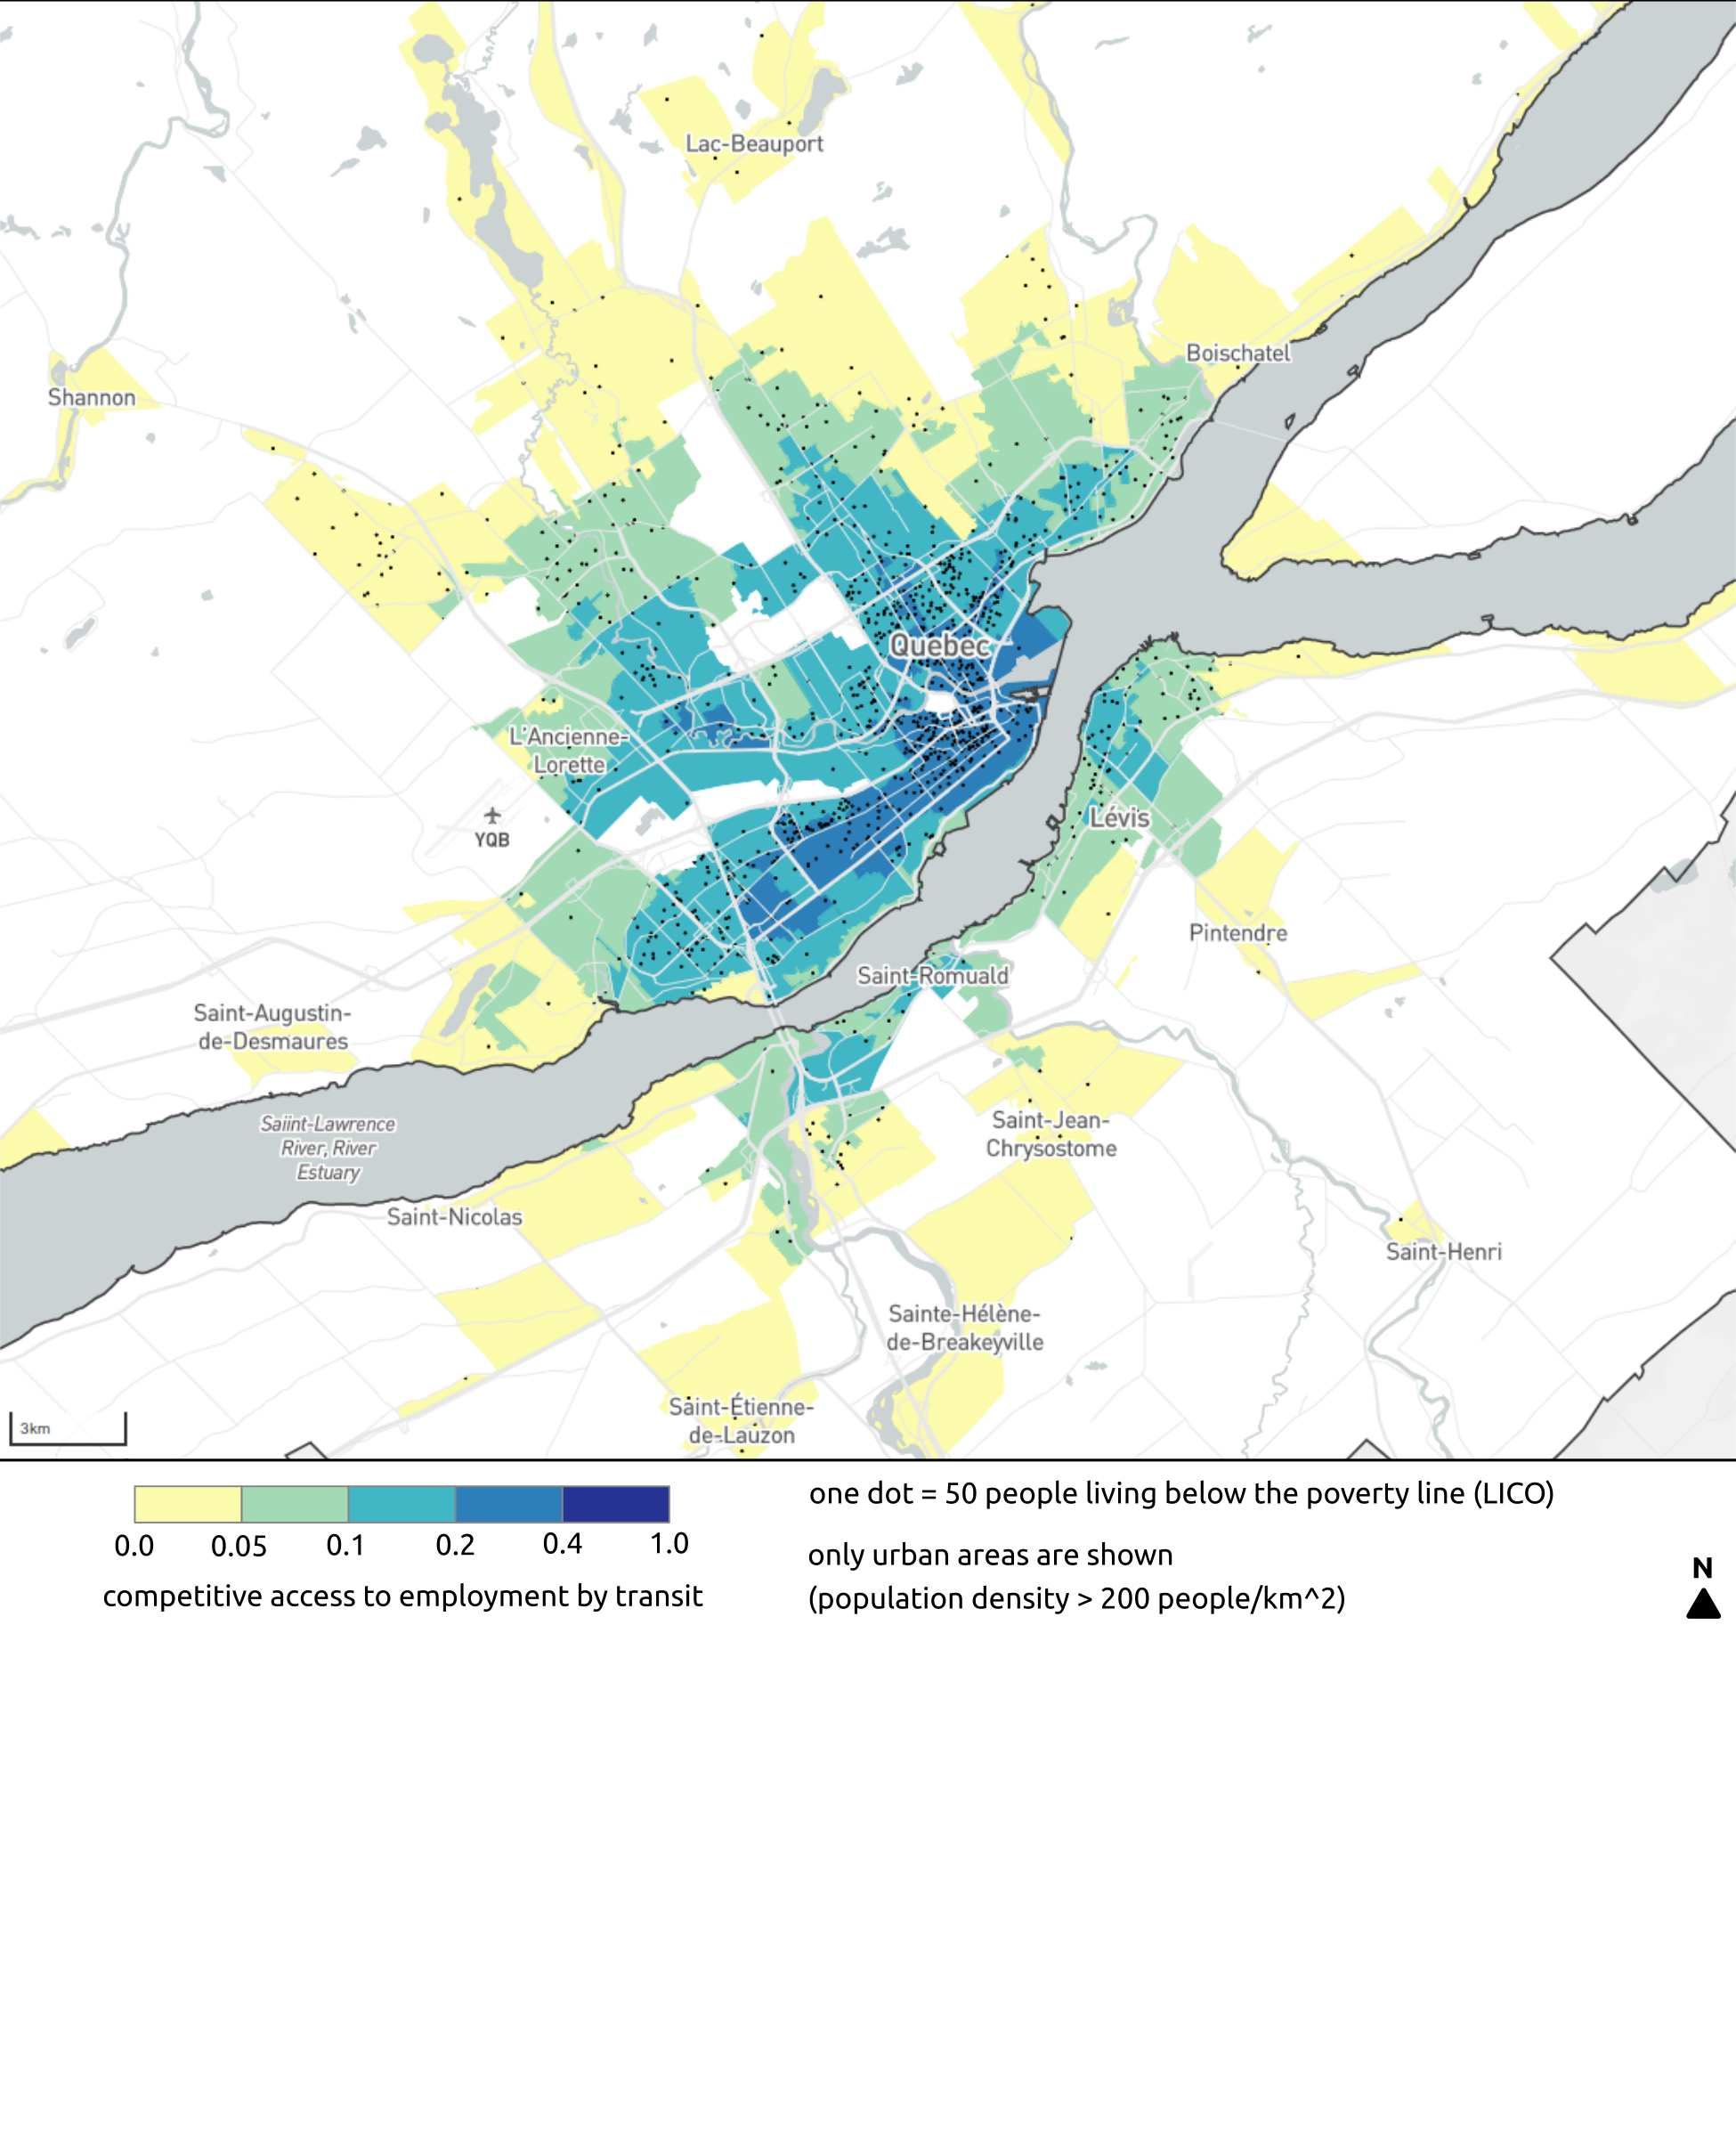
\includegraphics[width=6.5in]{figures/appendix_maps/a_que.png}}
\end{figure}

\begin{figure}[H]
	\vspace{5mm}
	\caption{Map of Montreal showing transit access to employment and low income households} 
	\label{a_van}
	\centerline{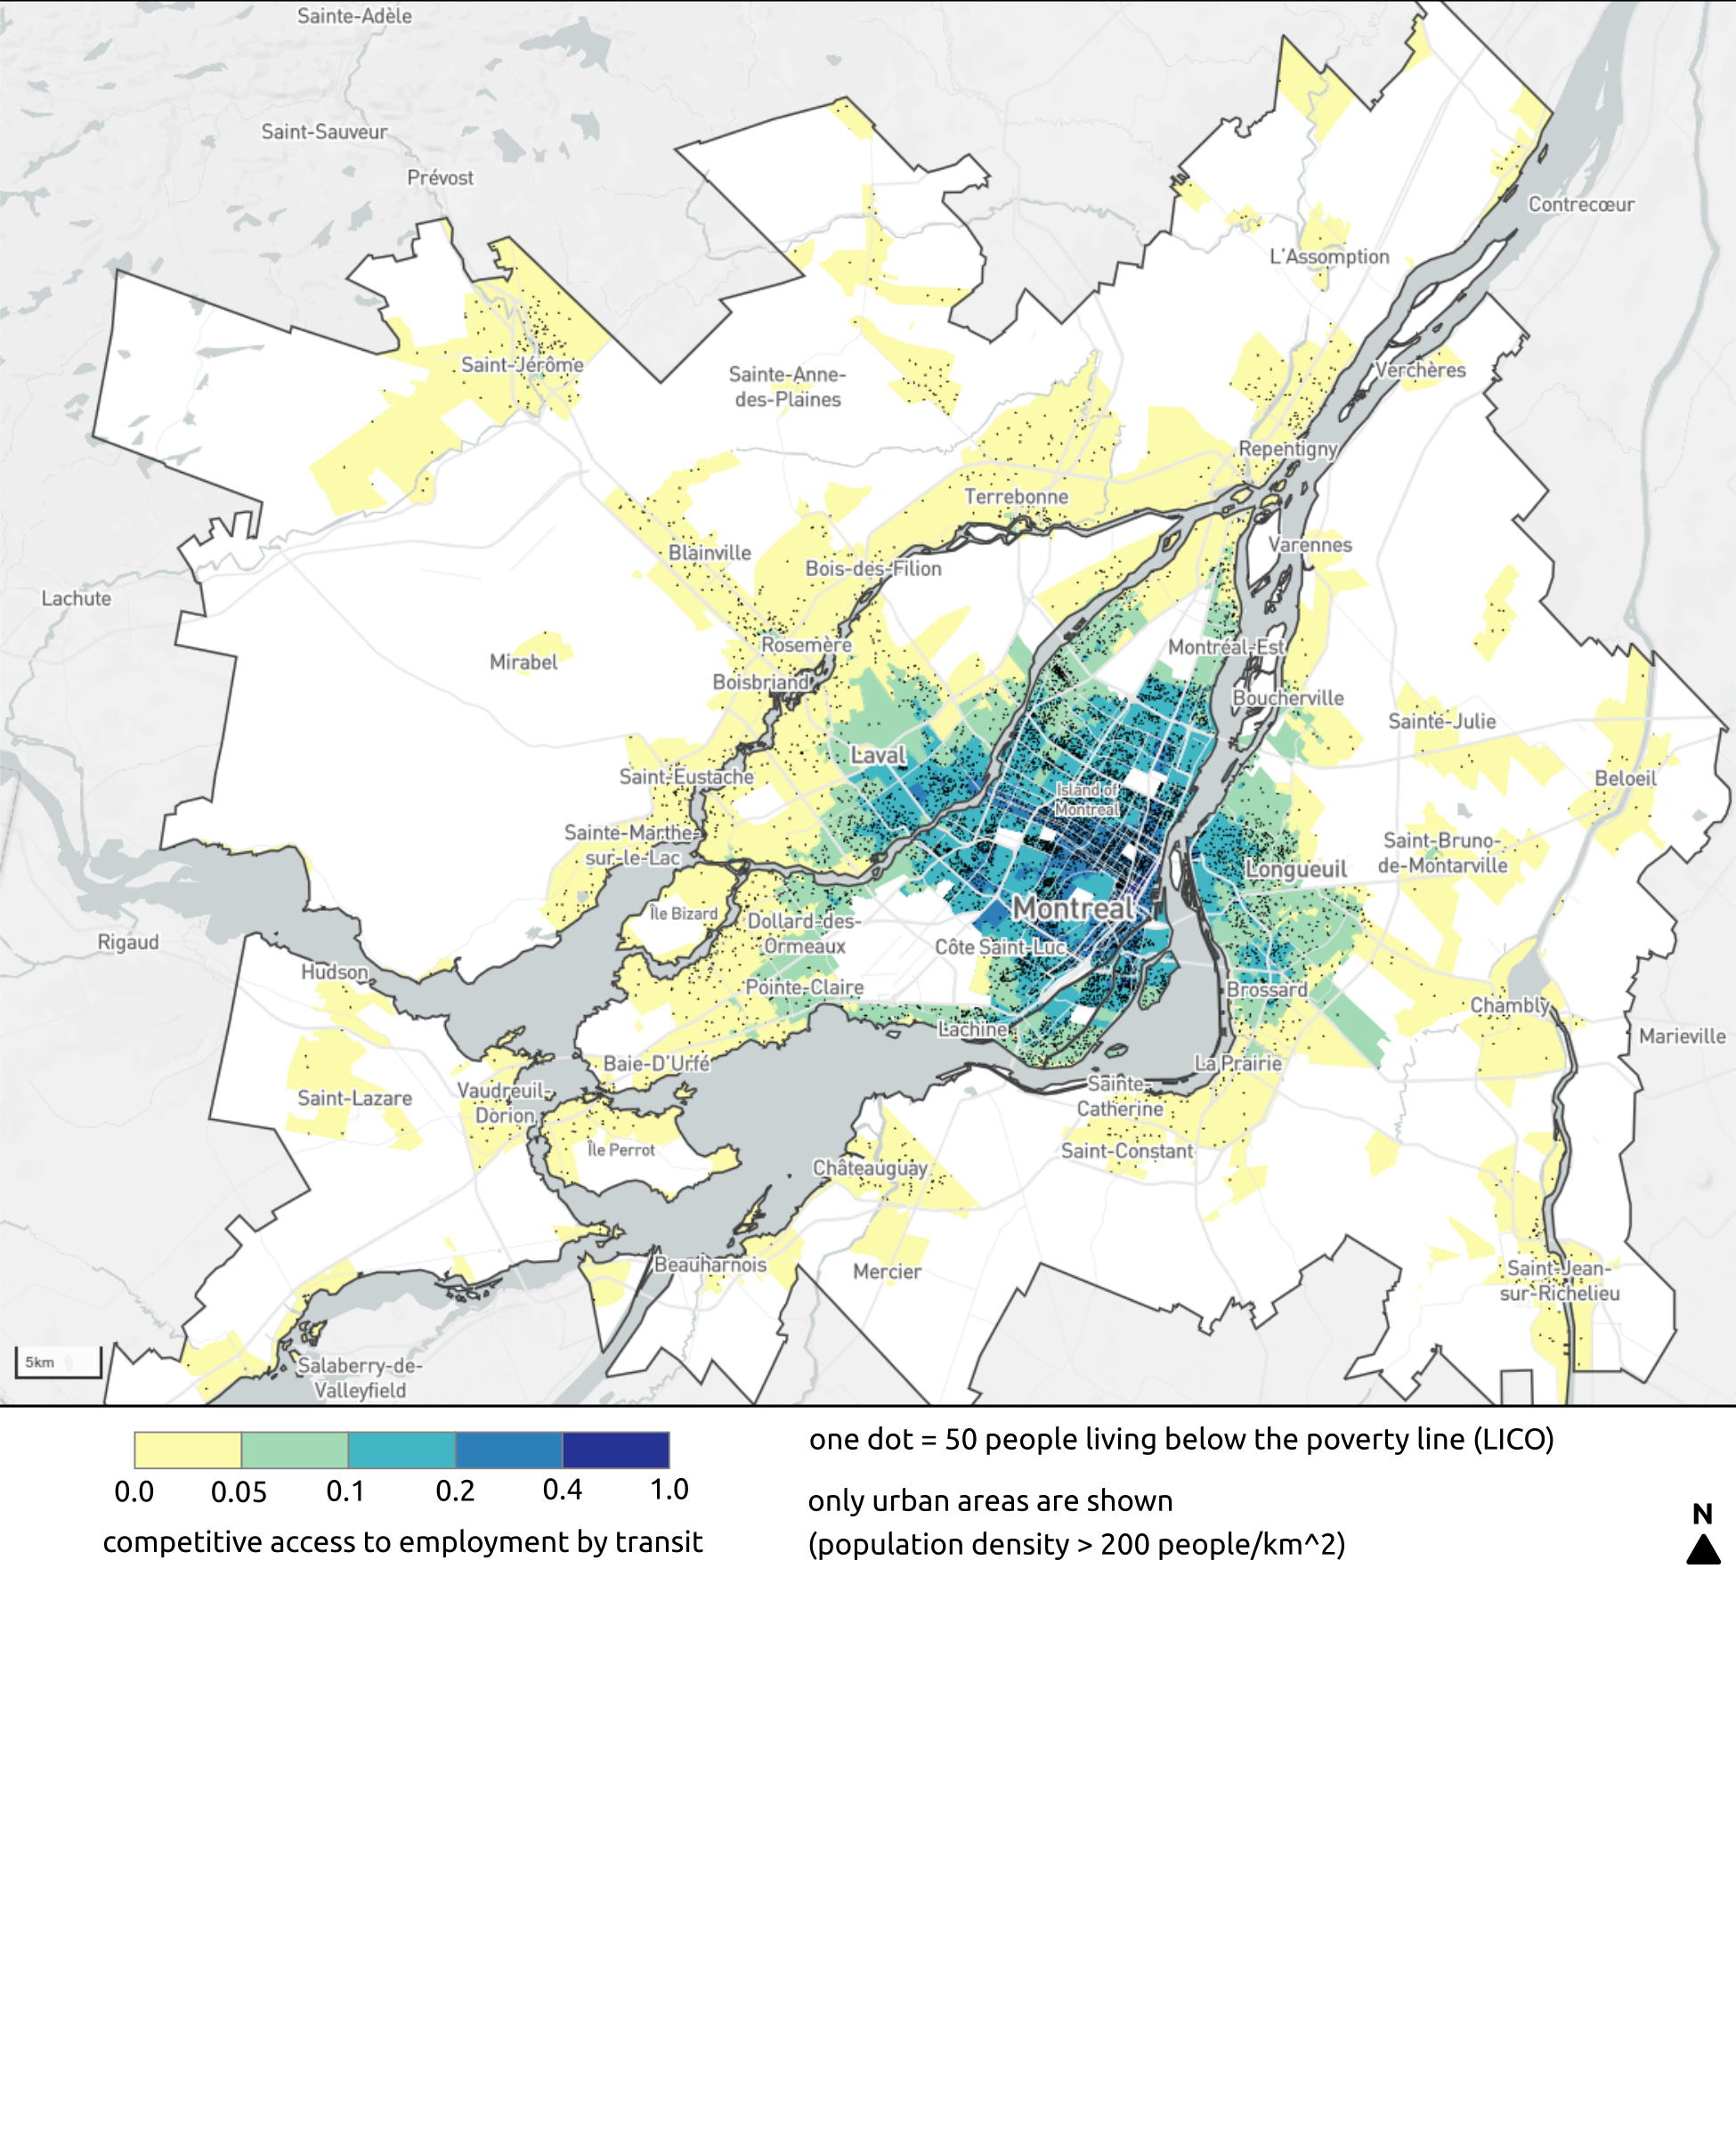
\includegraphics[width=6.5in]{figures/appendix_maps/a_mtl.png}}
\end{figure}

\begin{figure}[H]
	\vspace{5mm}
	\caption{Map of Ottawa showing transit access to employment and low income households} 
	\label{a_van}
	\centerline{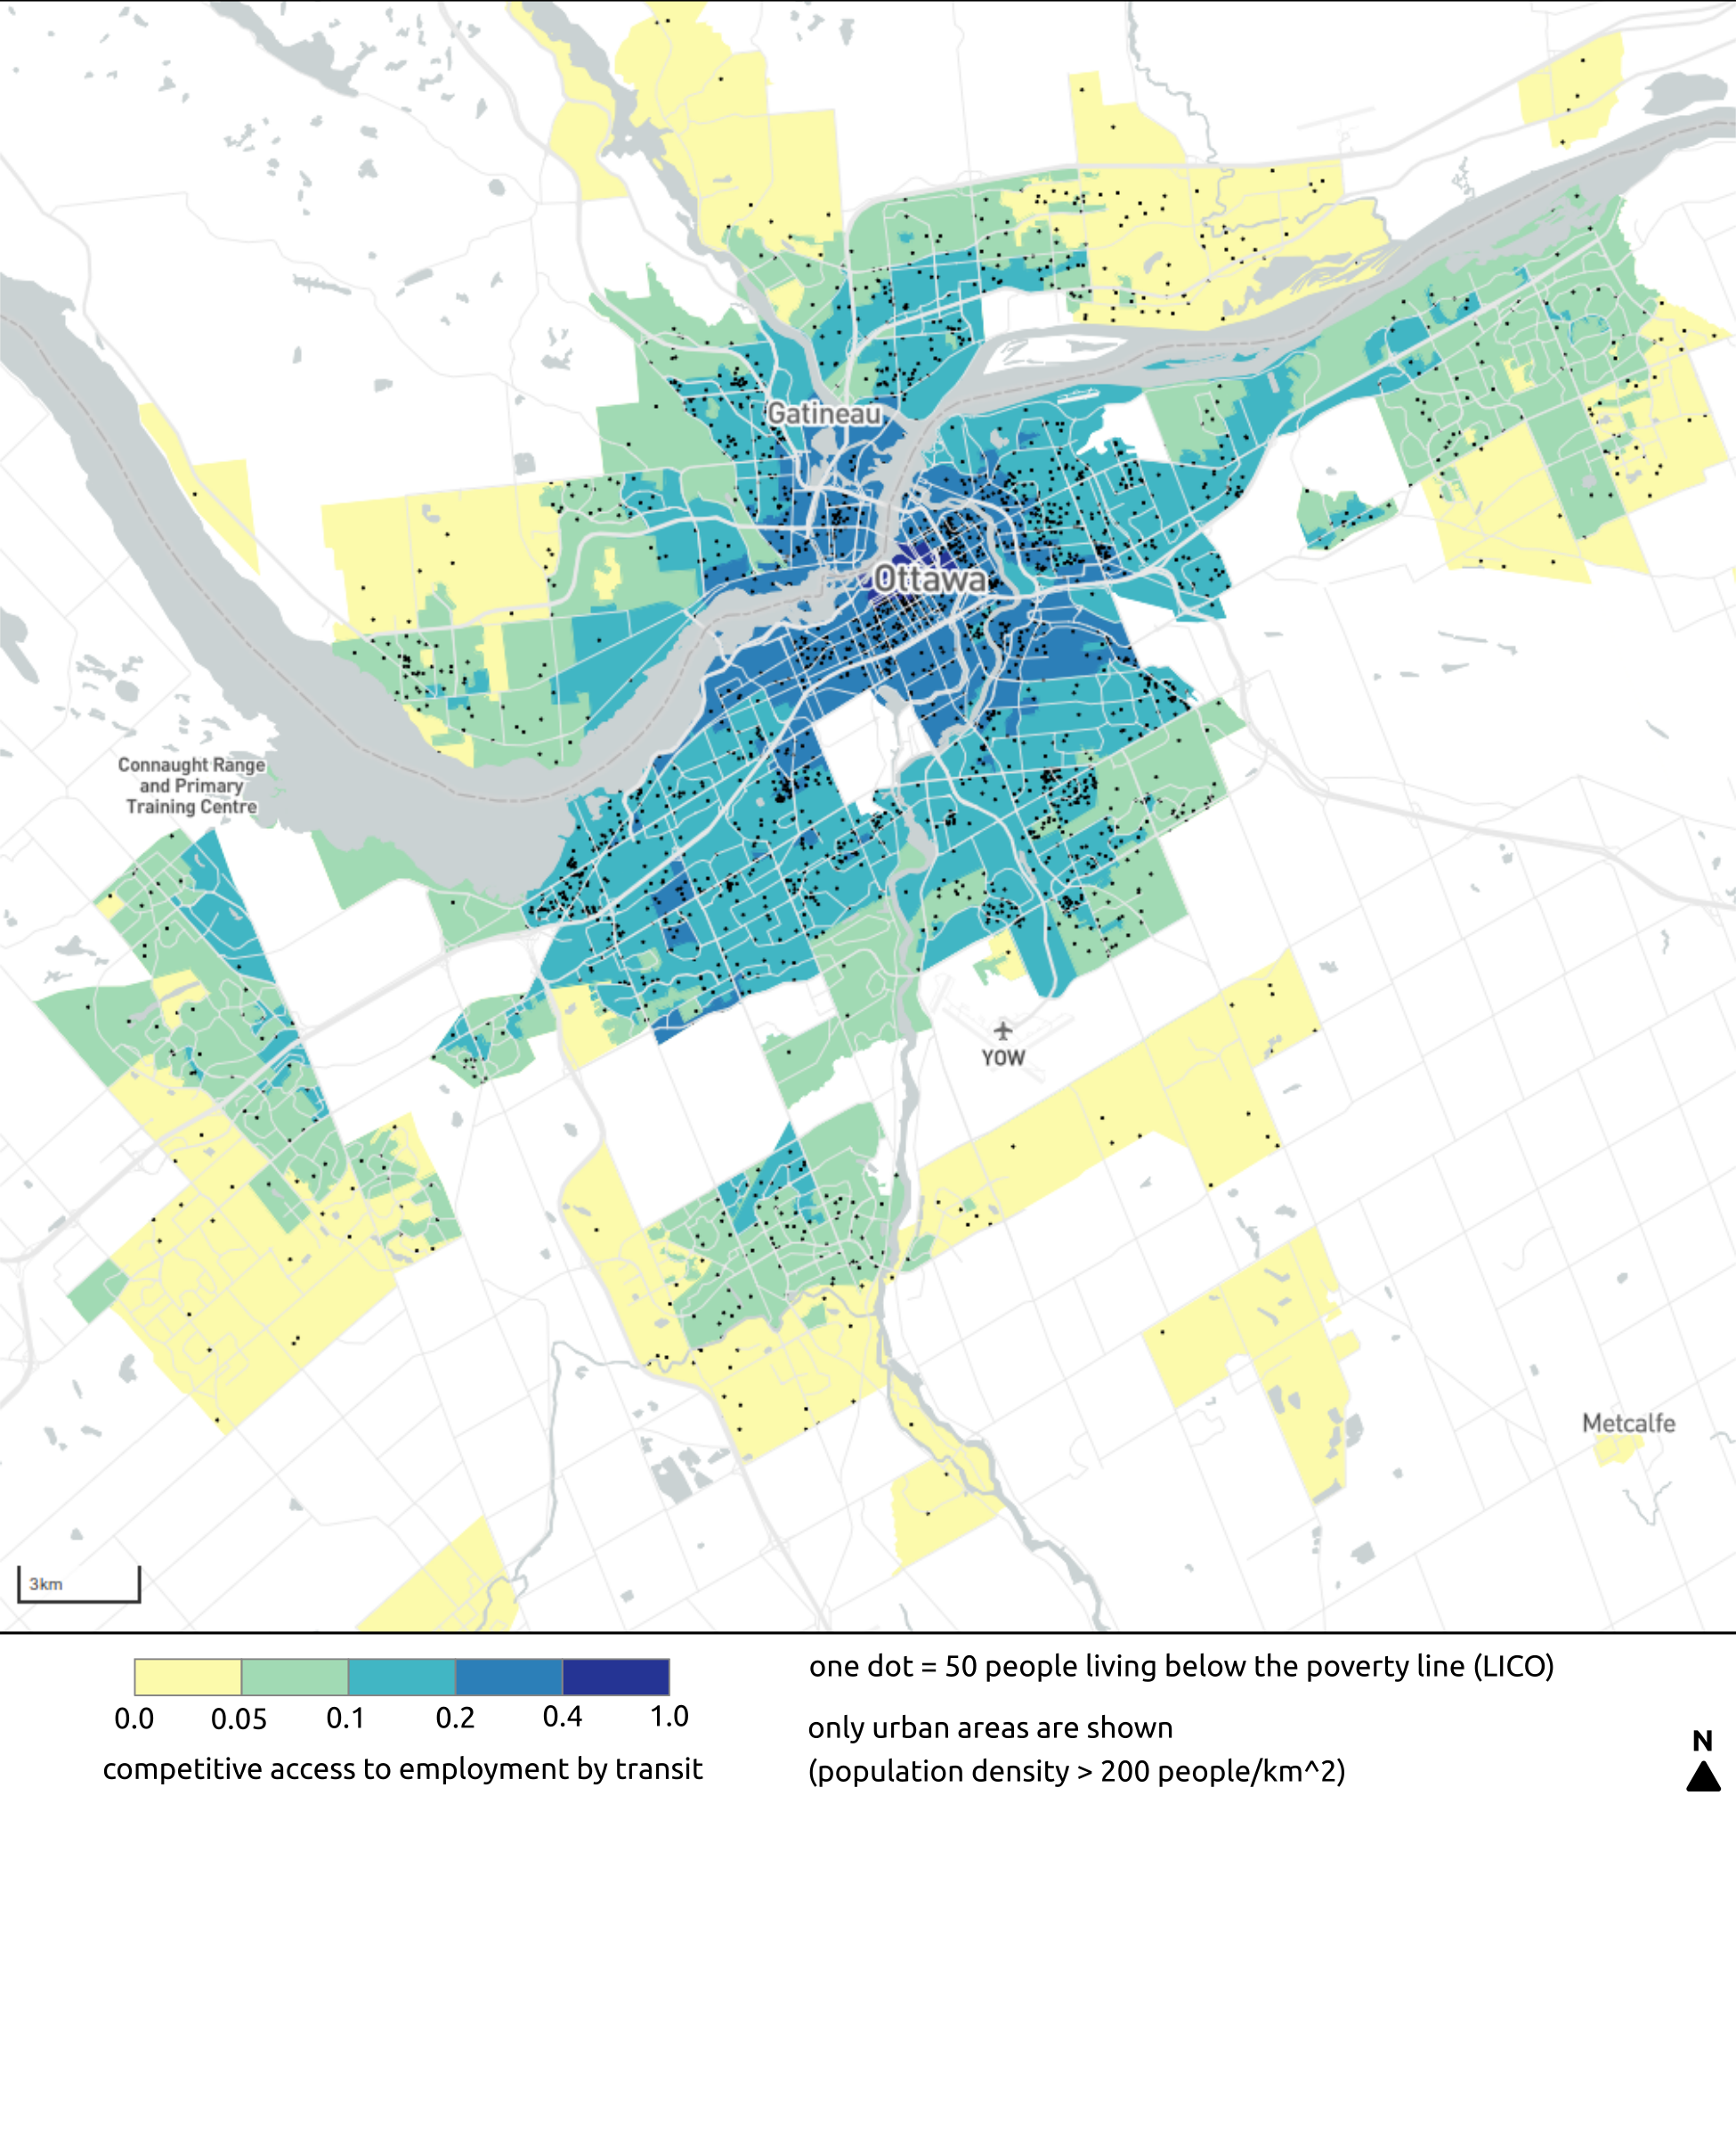
\includegraphics[width=6.5in]{figures/appendix_maps/a_ott.png}}
\end{figure}

\begin{figure}[H]
	\caption{Map of the Toronto region showingtransit access to employment and low income households} 
	\label{a_van}
	\centerline{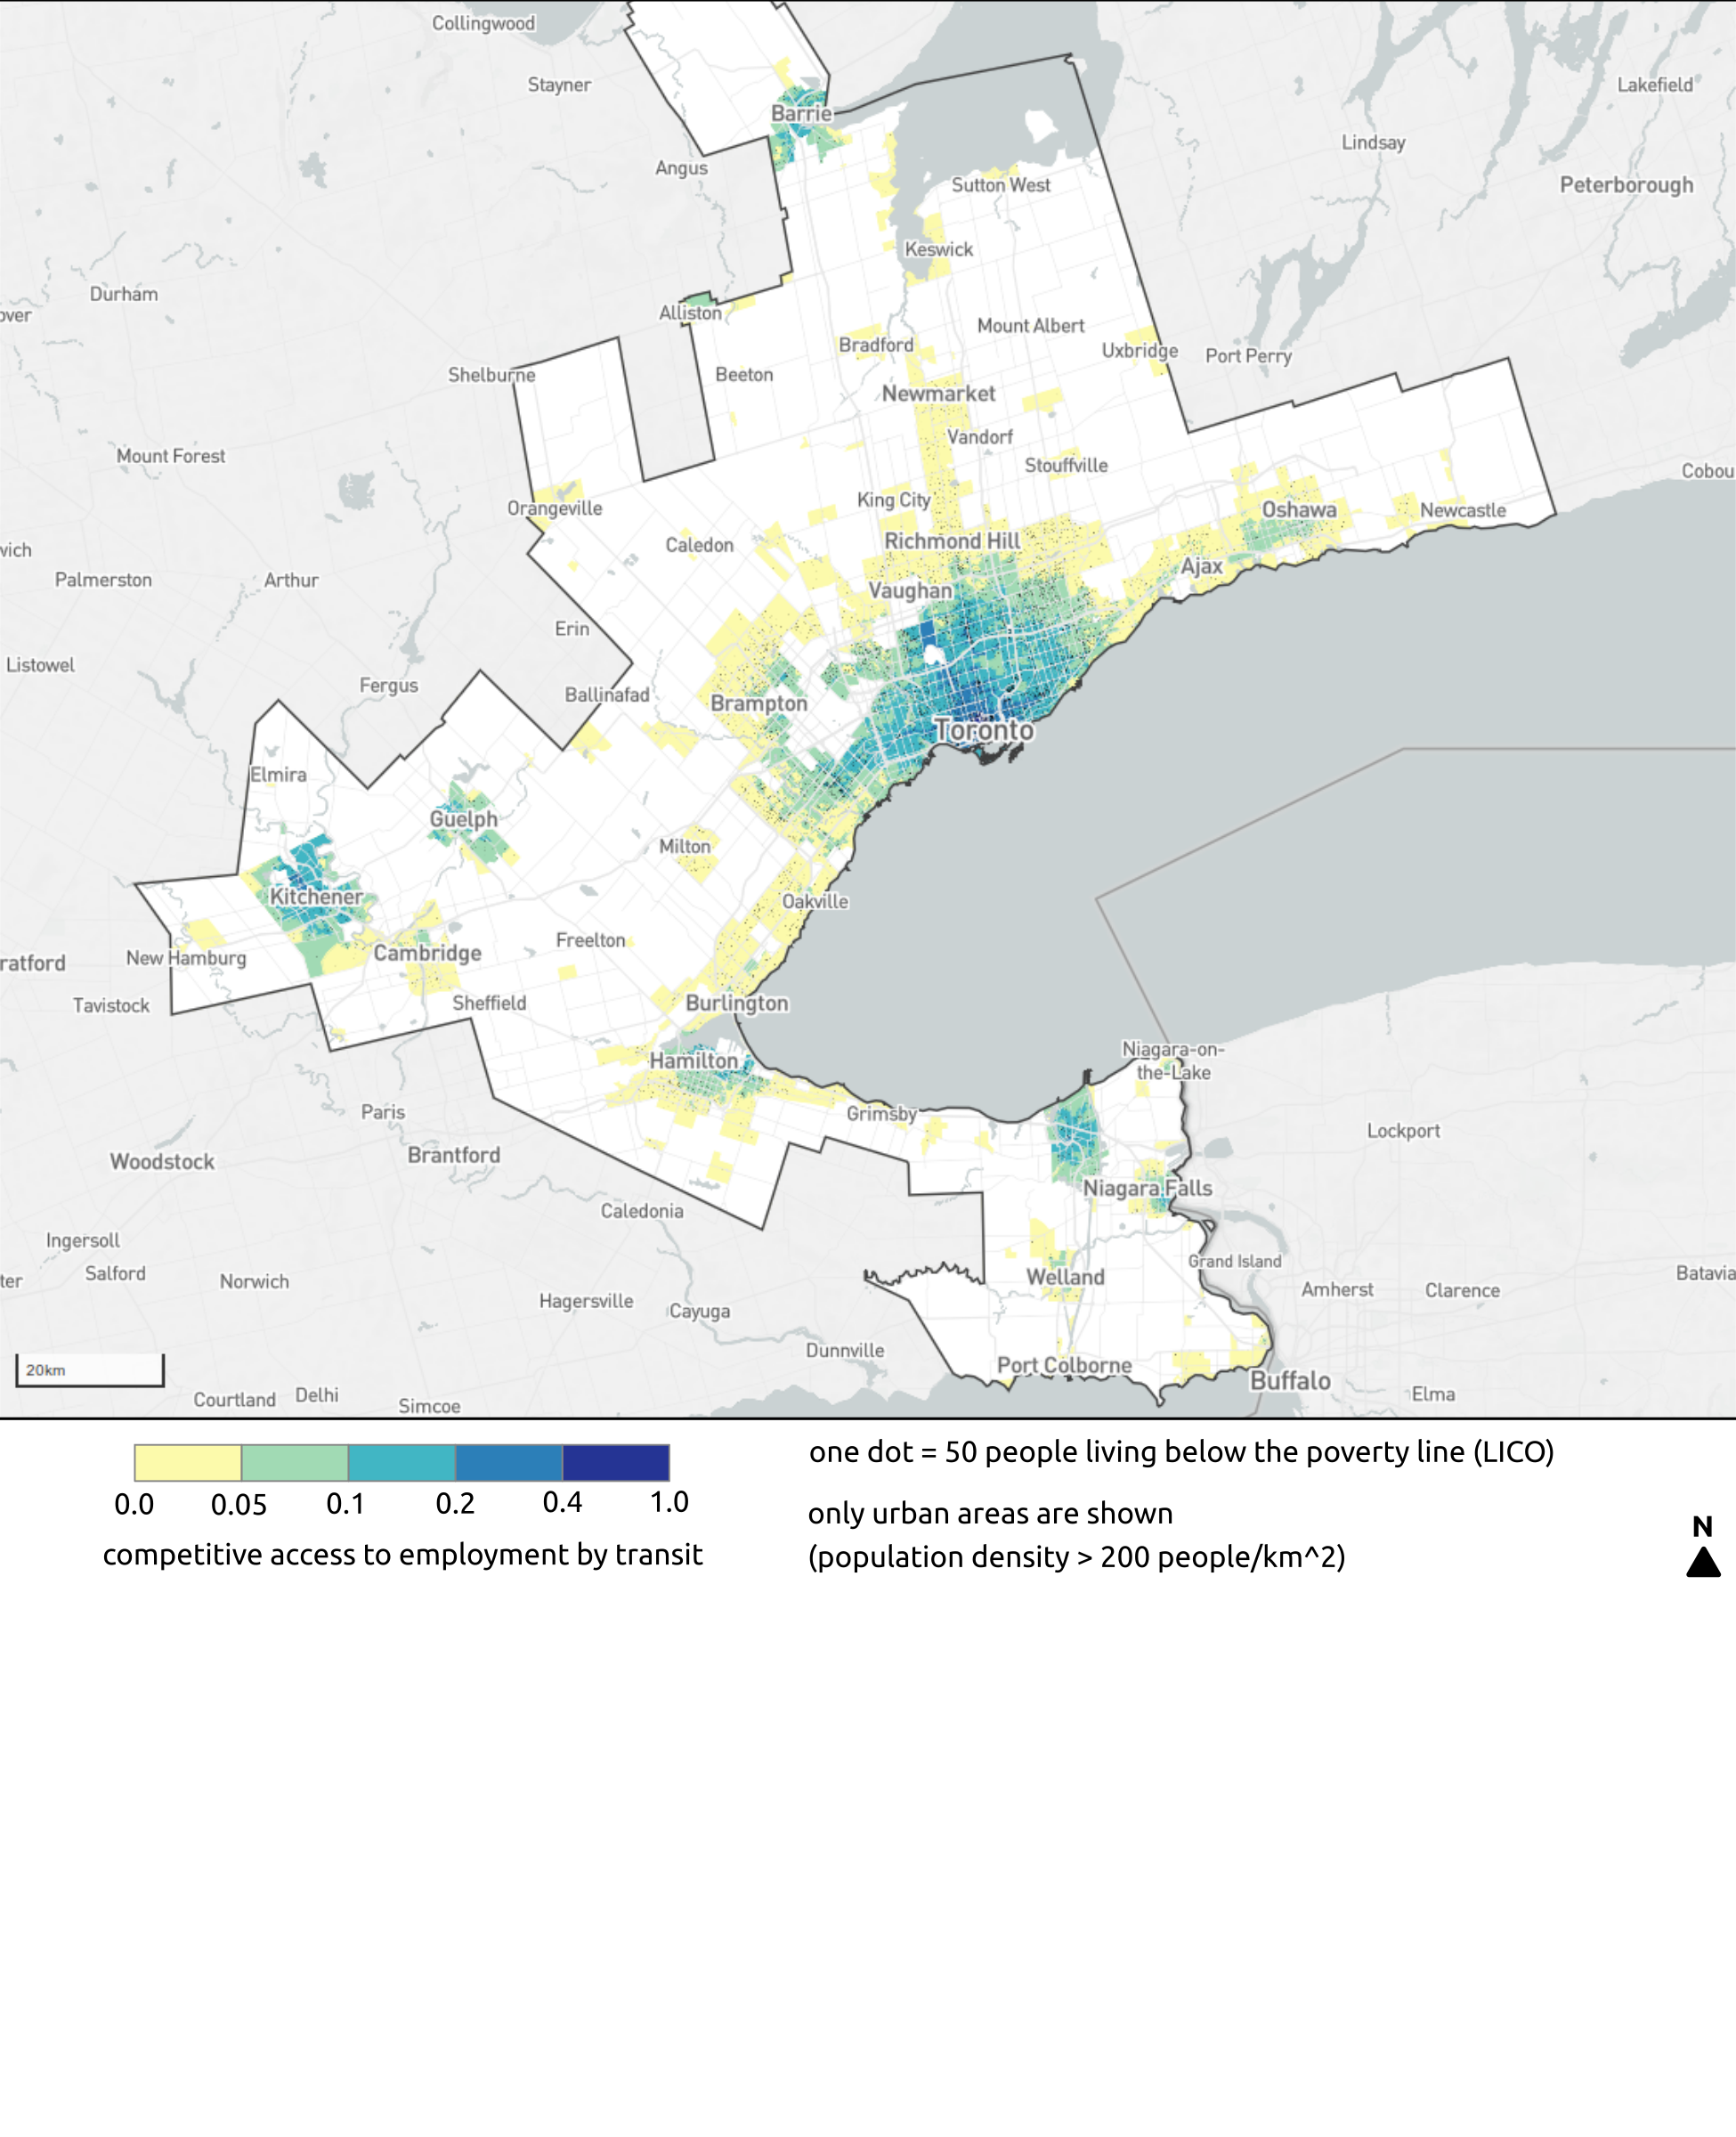
\includegraphics[width=6.5in]{figures/appendix_maps/a_tor_all.png}}
	\vspace{2mm}
\end{figure}

\begin{figure}[H]
	\caption{Map of Toronto centre showing transit access to employment and low income households} 
	\label{a_van}
	\centerline{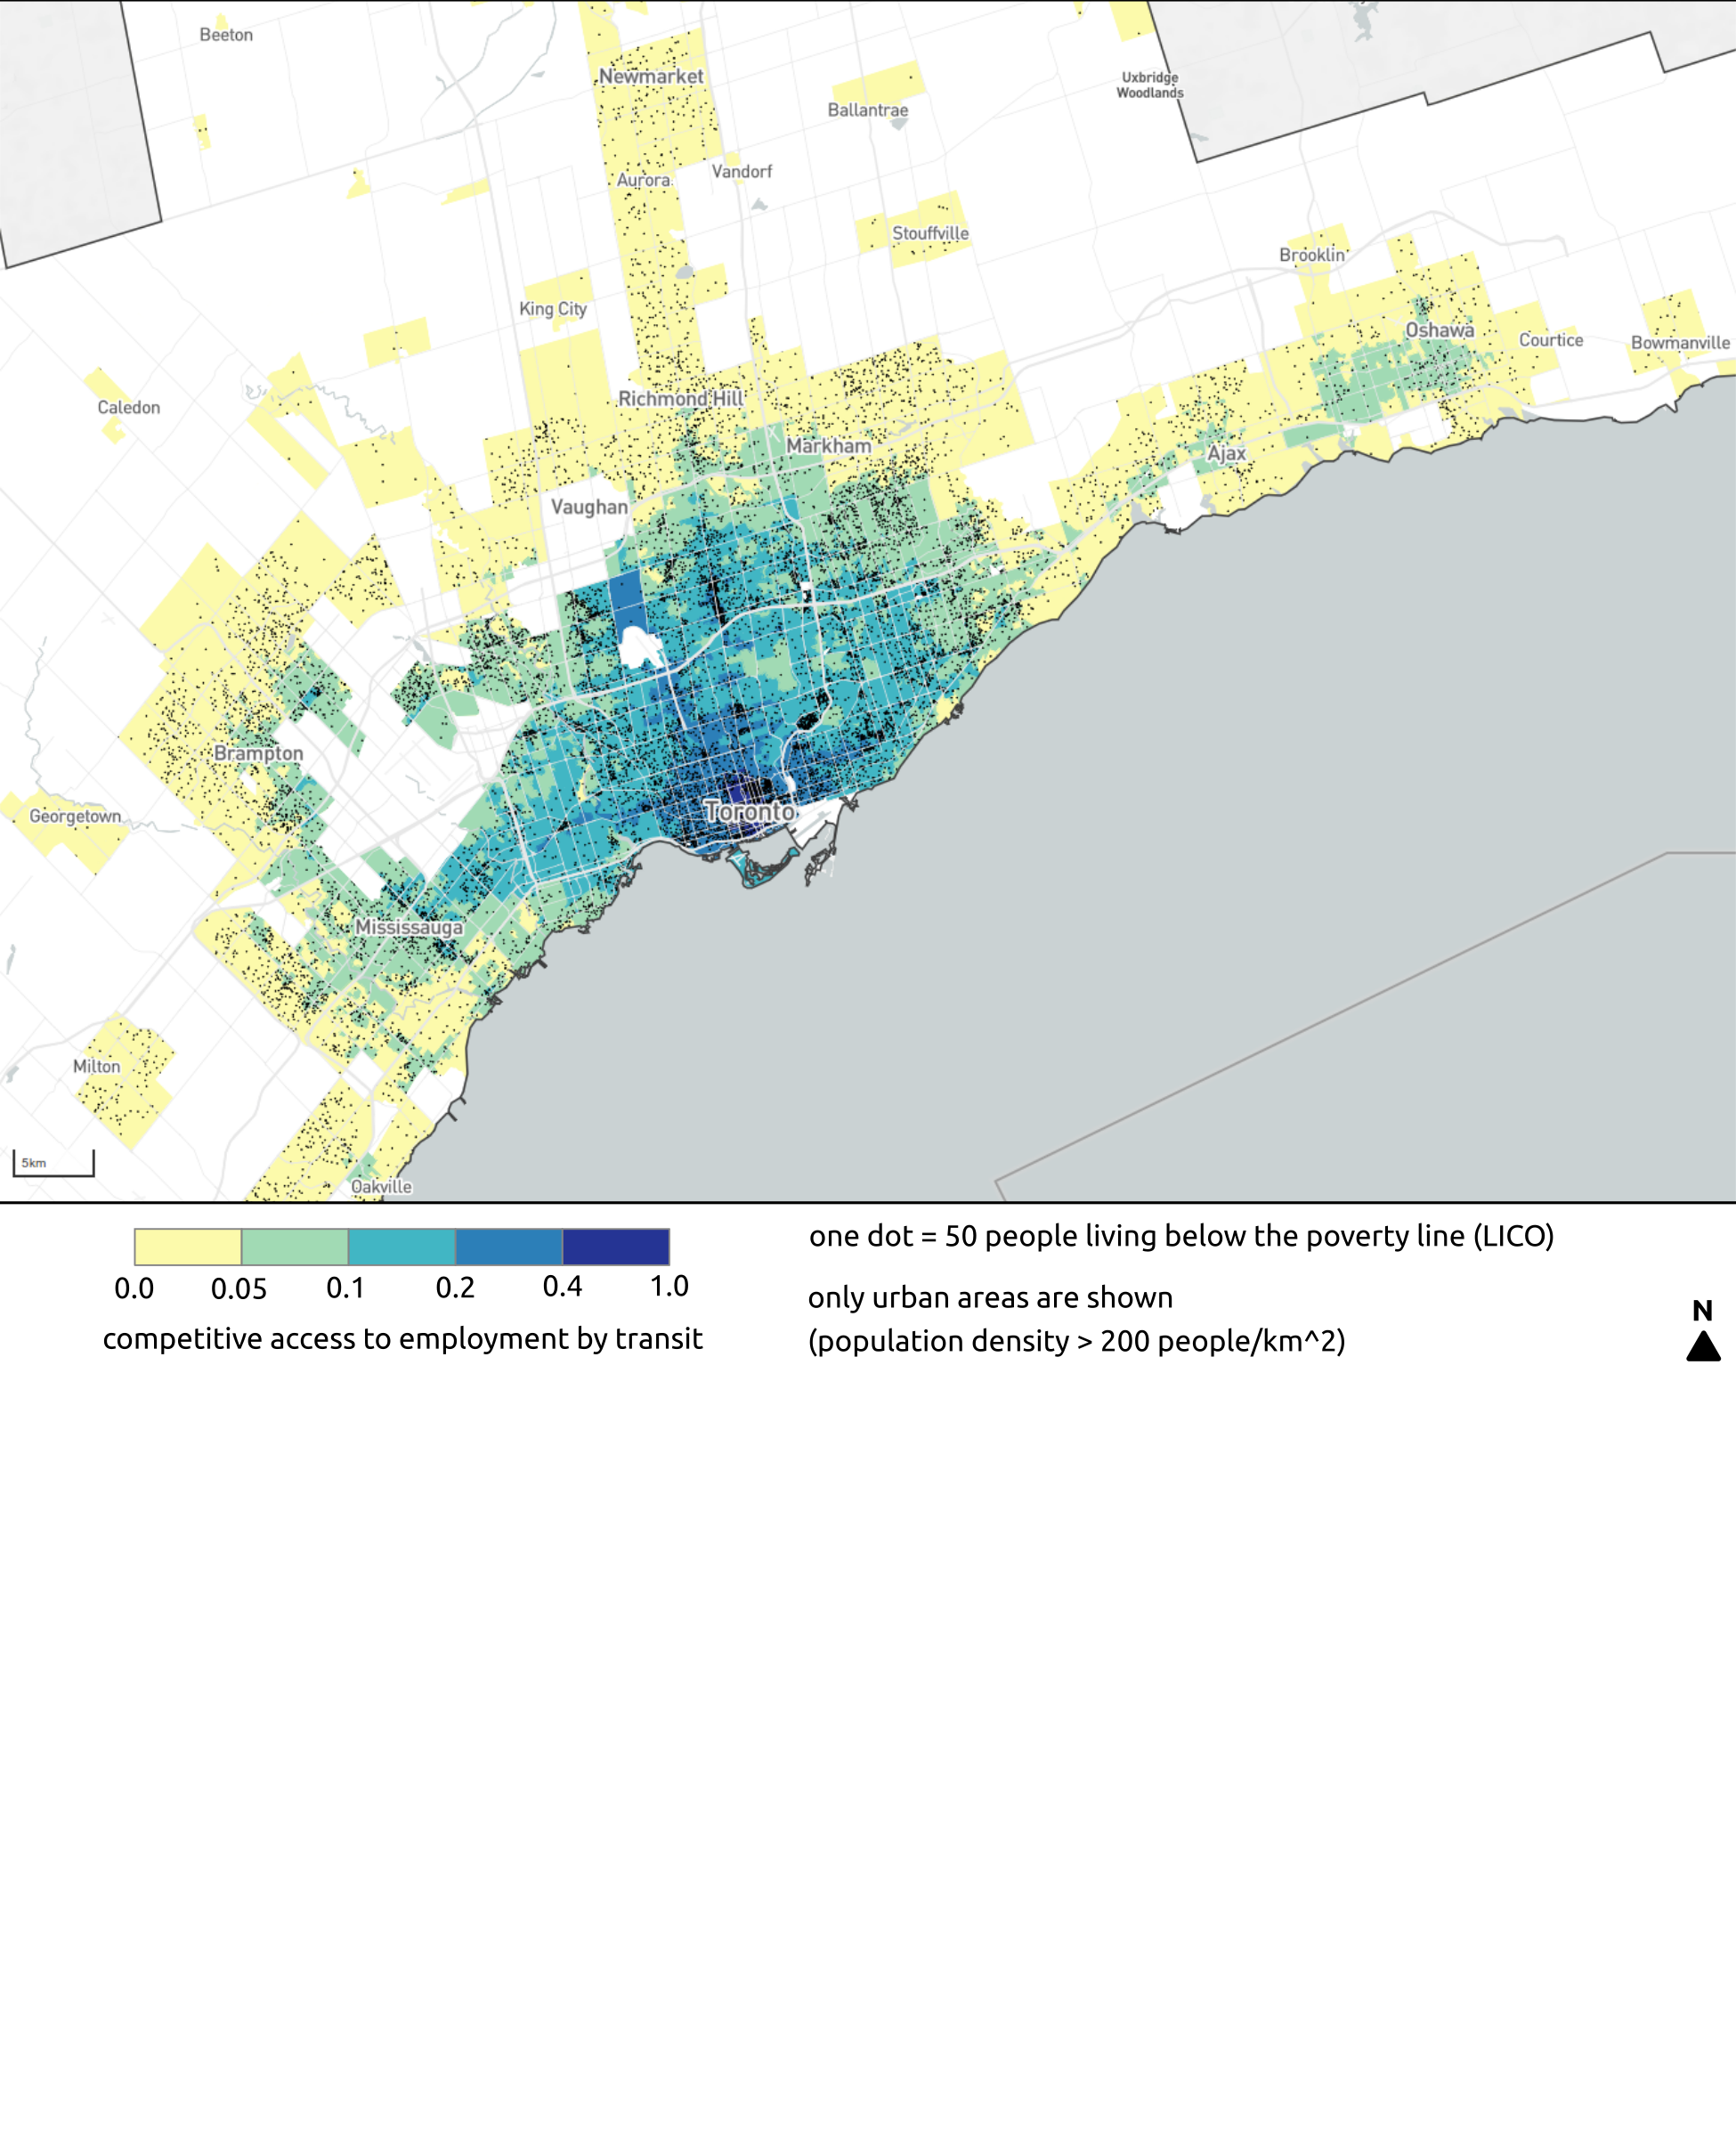
\includegraphics[width=6.5in]{figures/appendix_maps/a_tor_centre.png}}
	\vspace{2mm}
\end{figure}

\begin{figure}[H]
	\caption{Map of Hamilton, Guelph, and Kitchener-Waterloo showing transit access to employment and low income households} 
	\label{a_van}
	\centerline{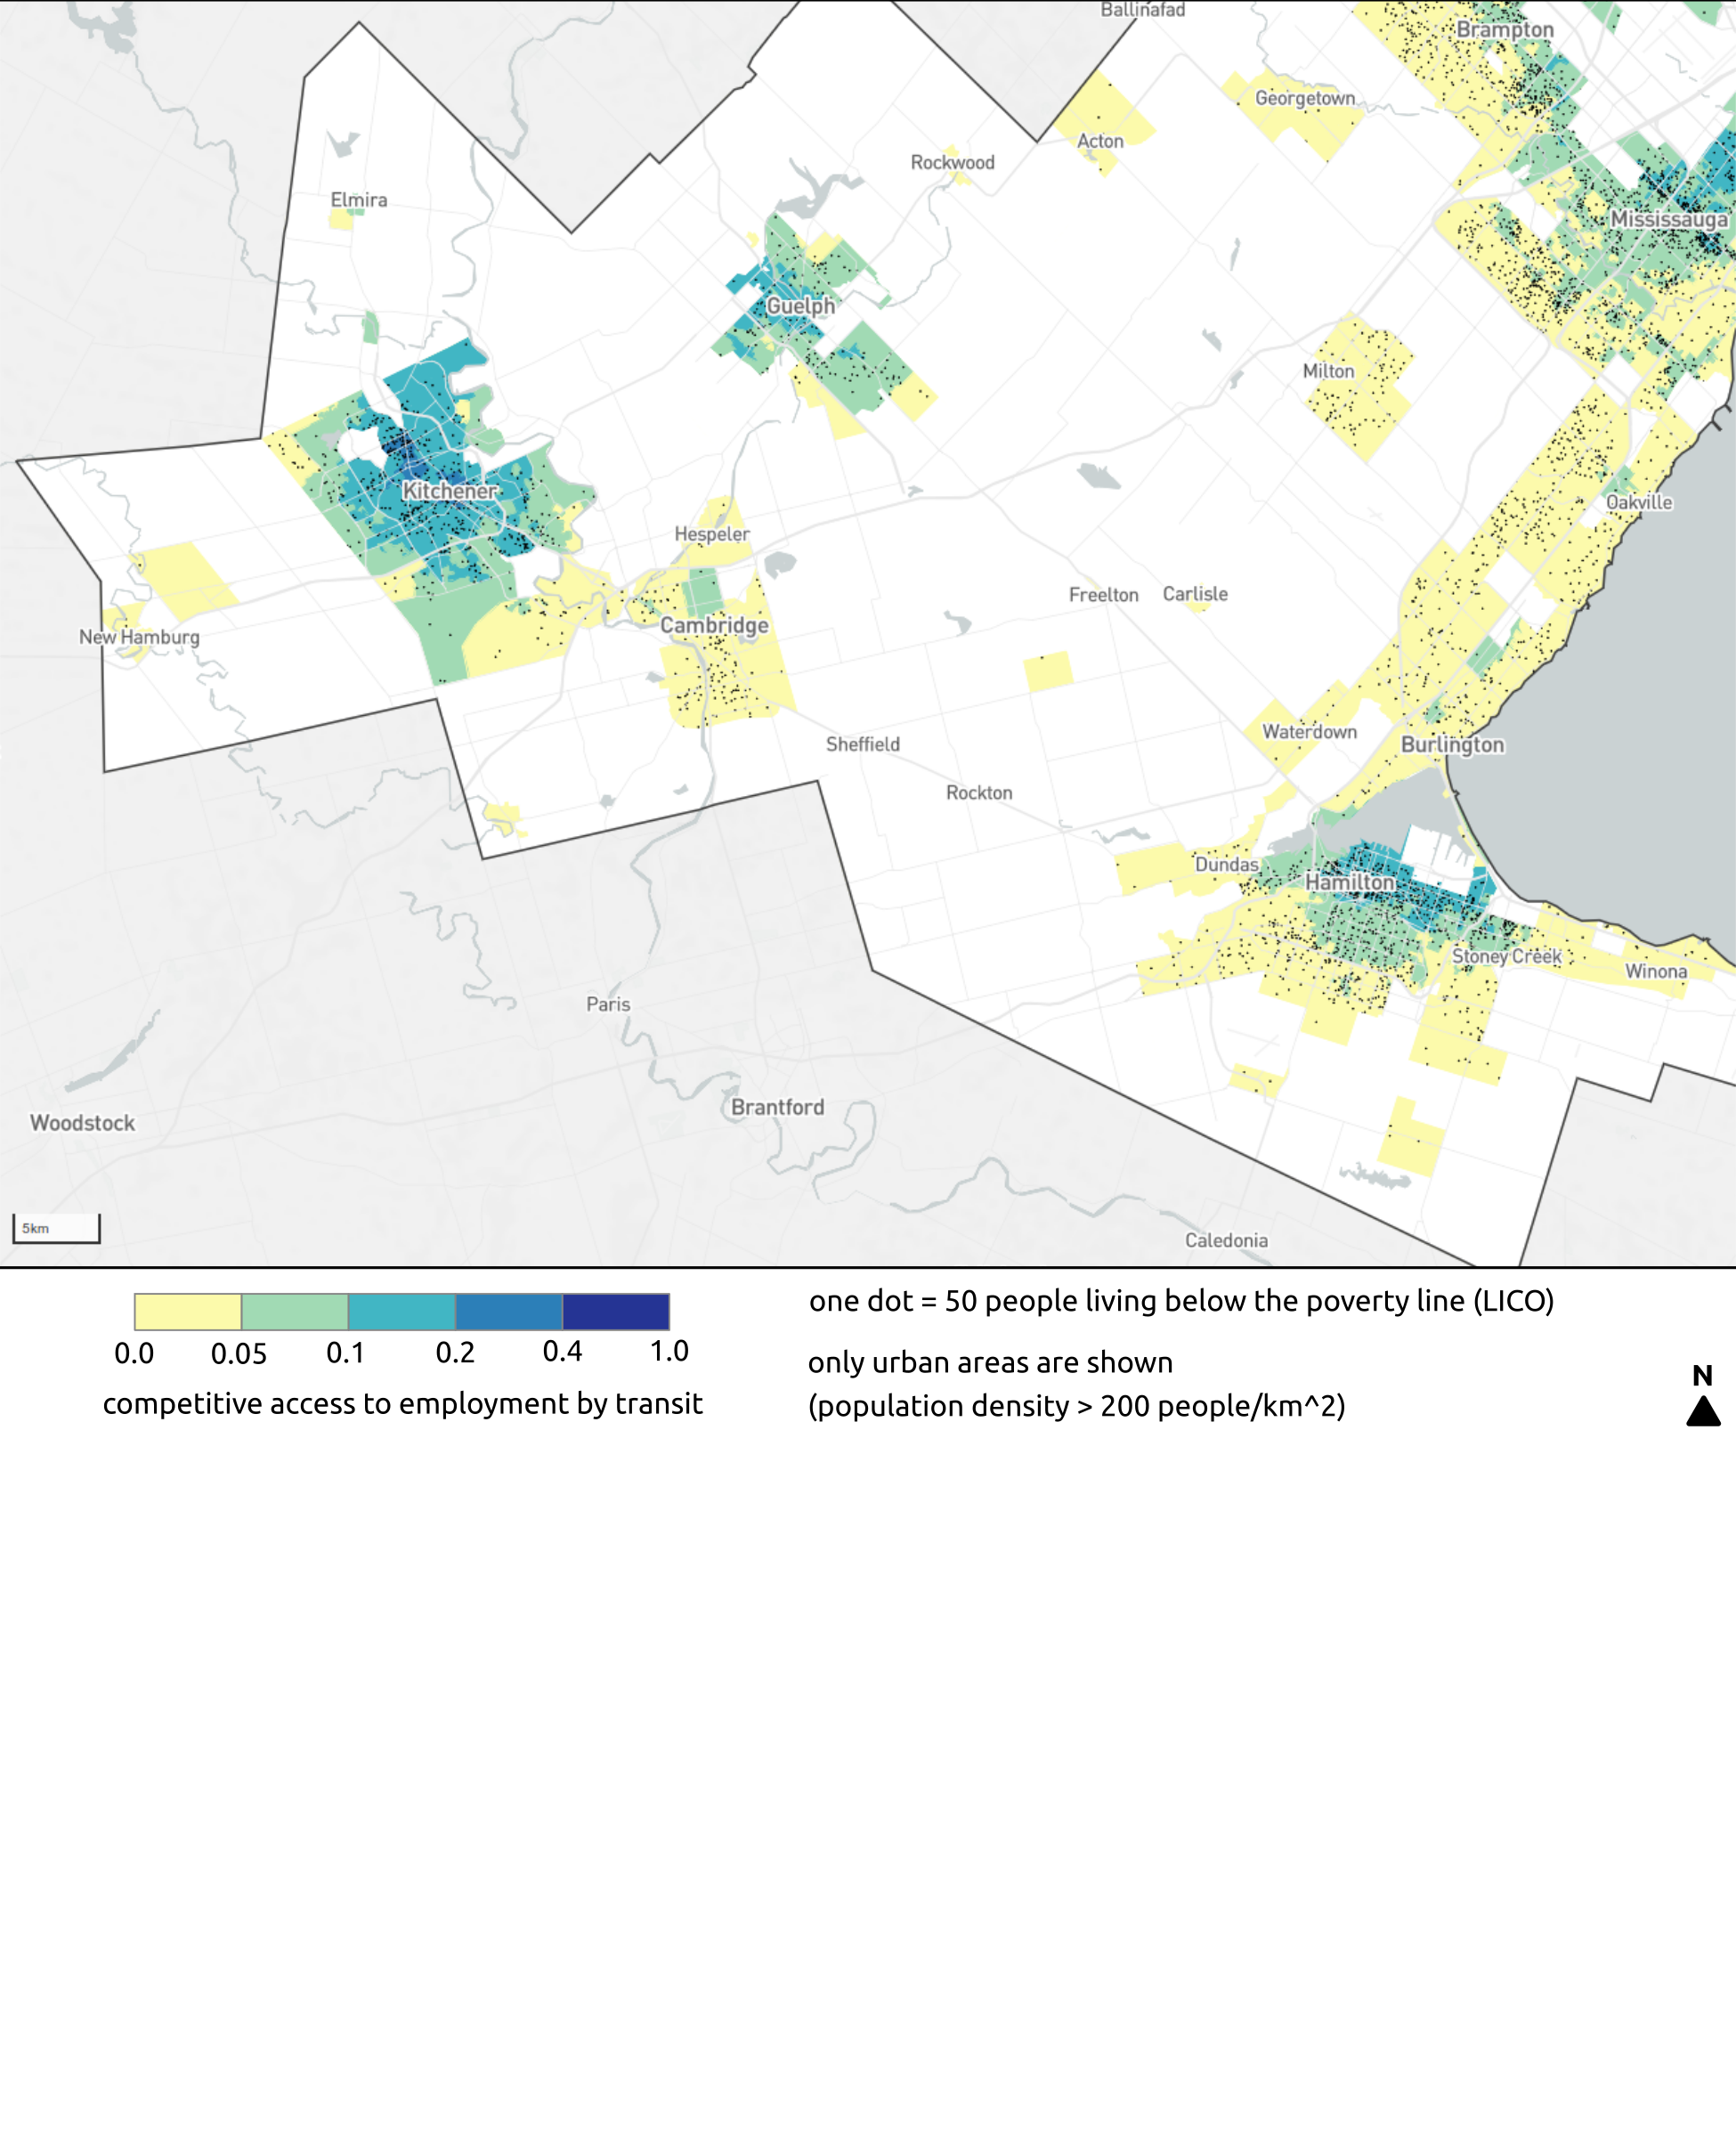
\includegraphics[width=6.5in]{figures/appendix_maps/a_tor_west.png}}
	\vspace{2mm}
\end{figure}


\begin{figure}[H]
	\caption{Map of Winnipeg showing transit access to employment and low income households} 
	\label{a_van}
	\centerline{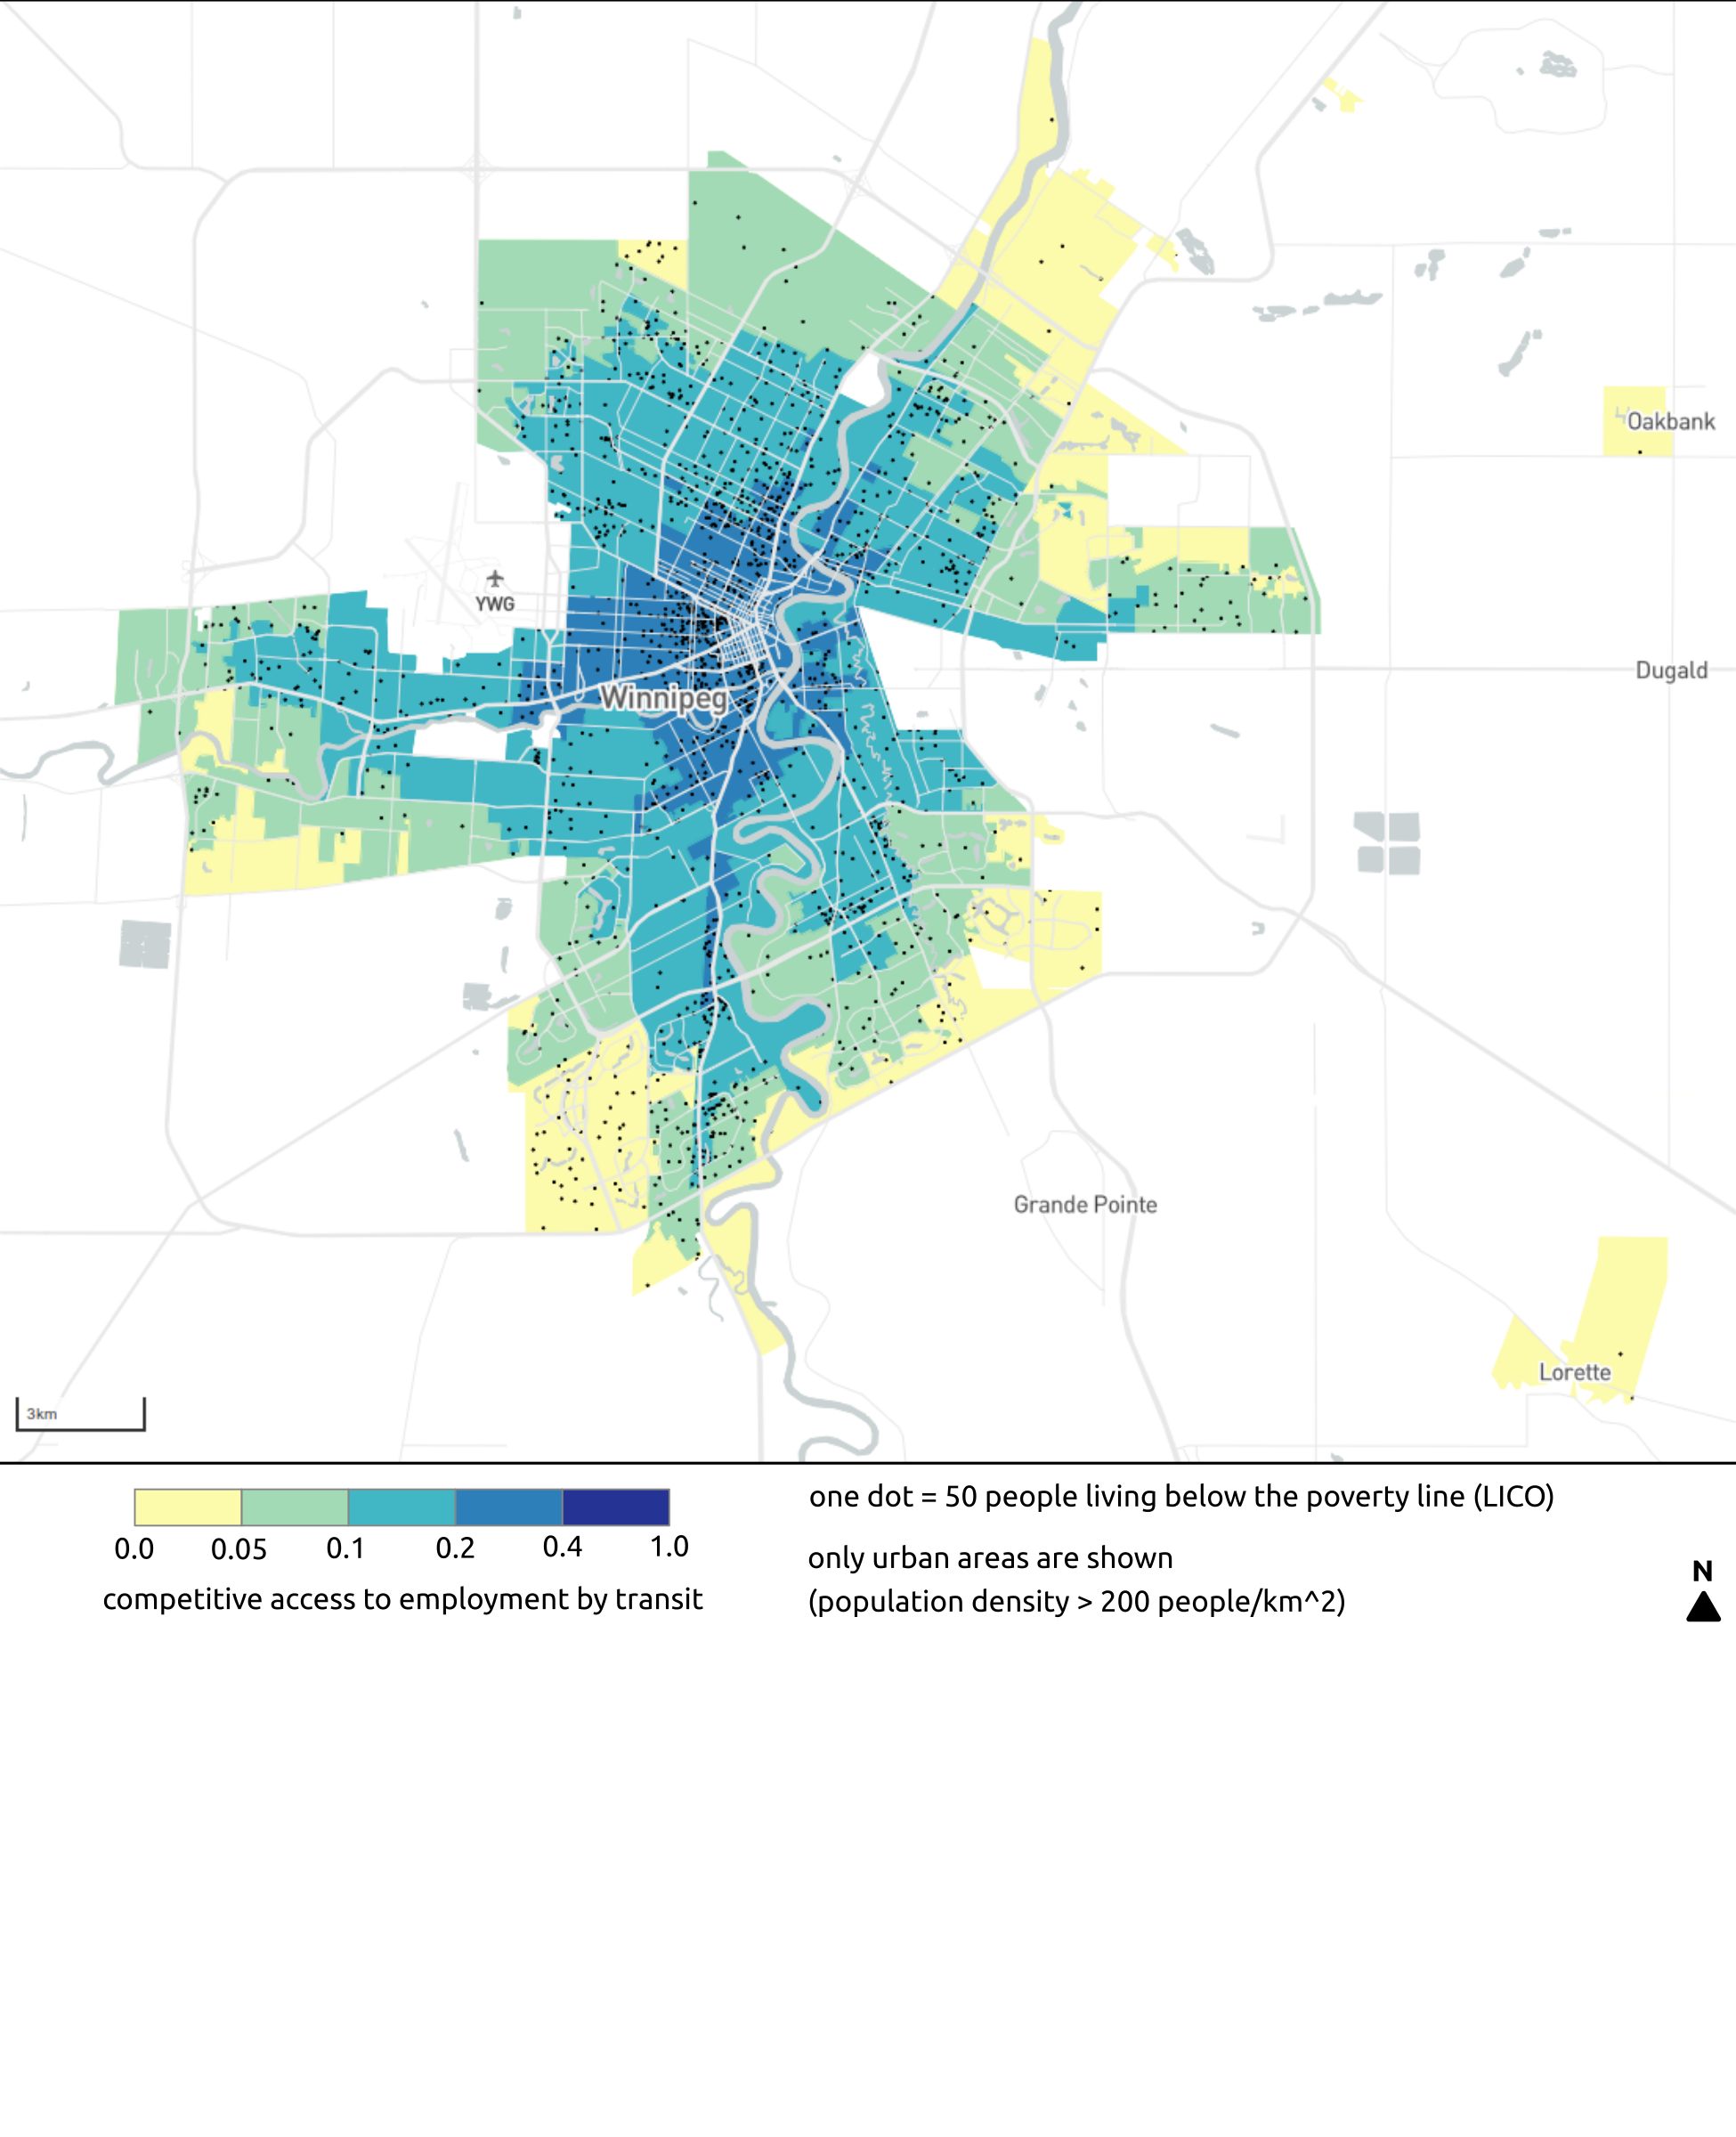
\includegraphics[width=6.5in]{figures/appendix_maps/a_wpg.png}}
	\vspace{2mm}
\end{figure}

\begin{figure}[H]
	\caption{Map of Calgary showing transit access to employment and low income households} 
	\label{a_van}
	\centerline{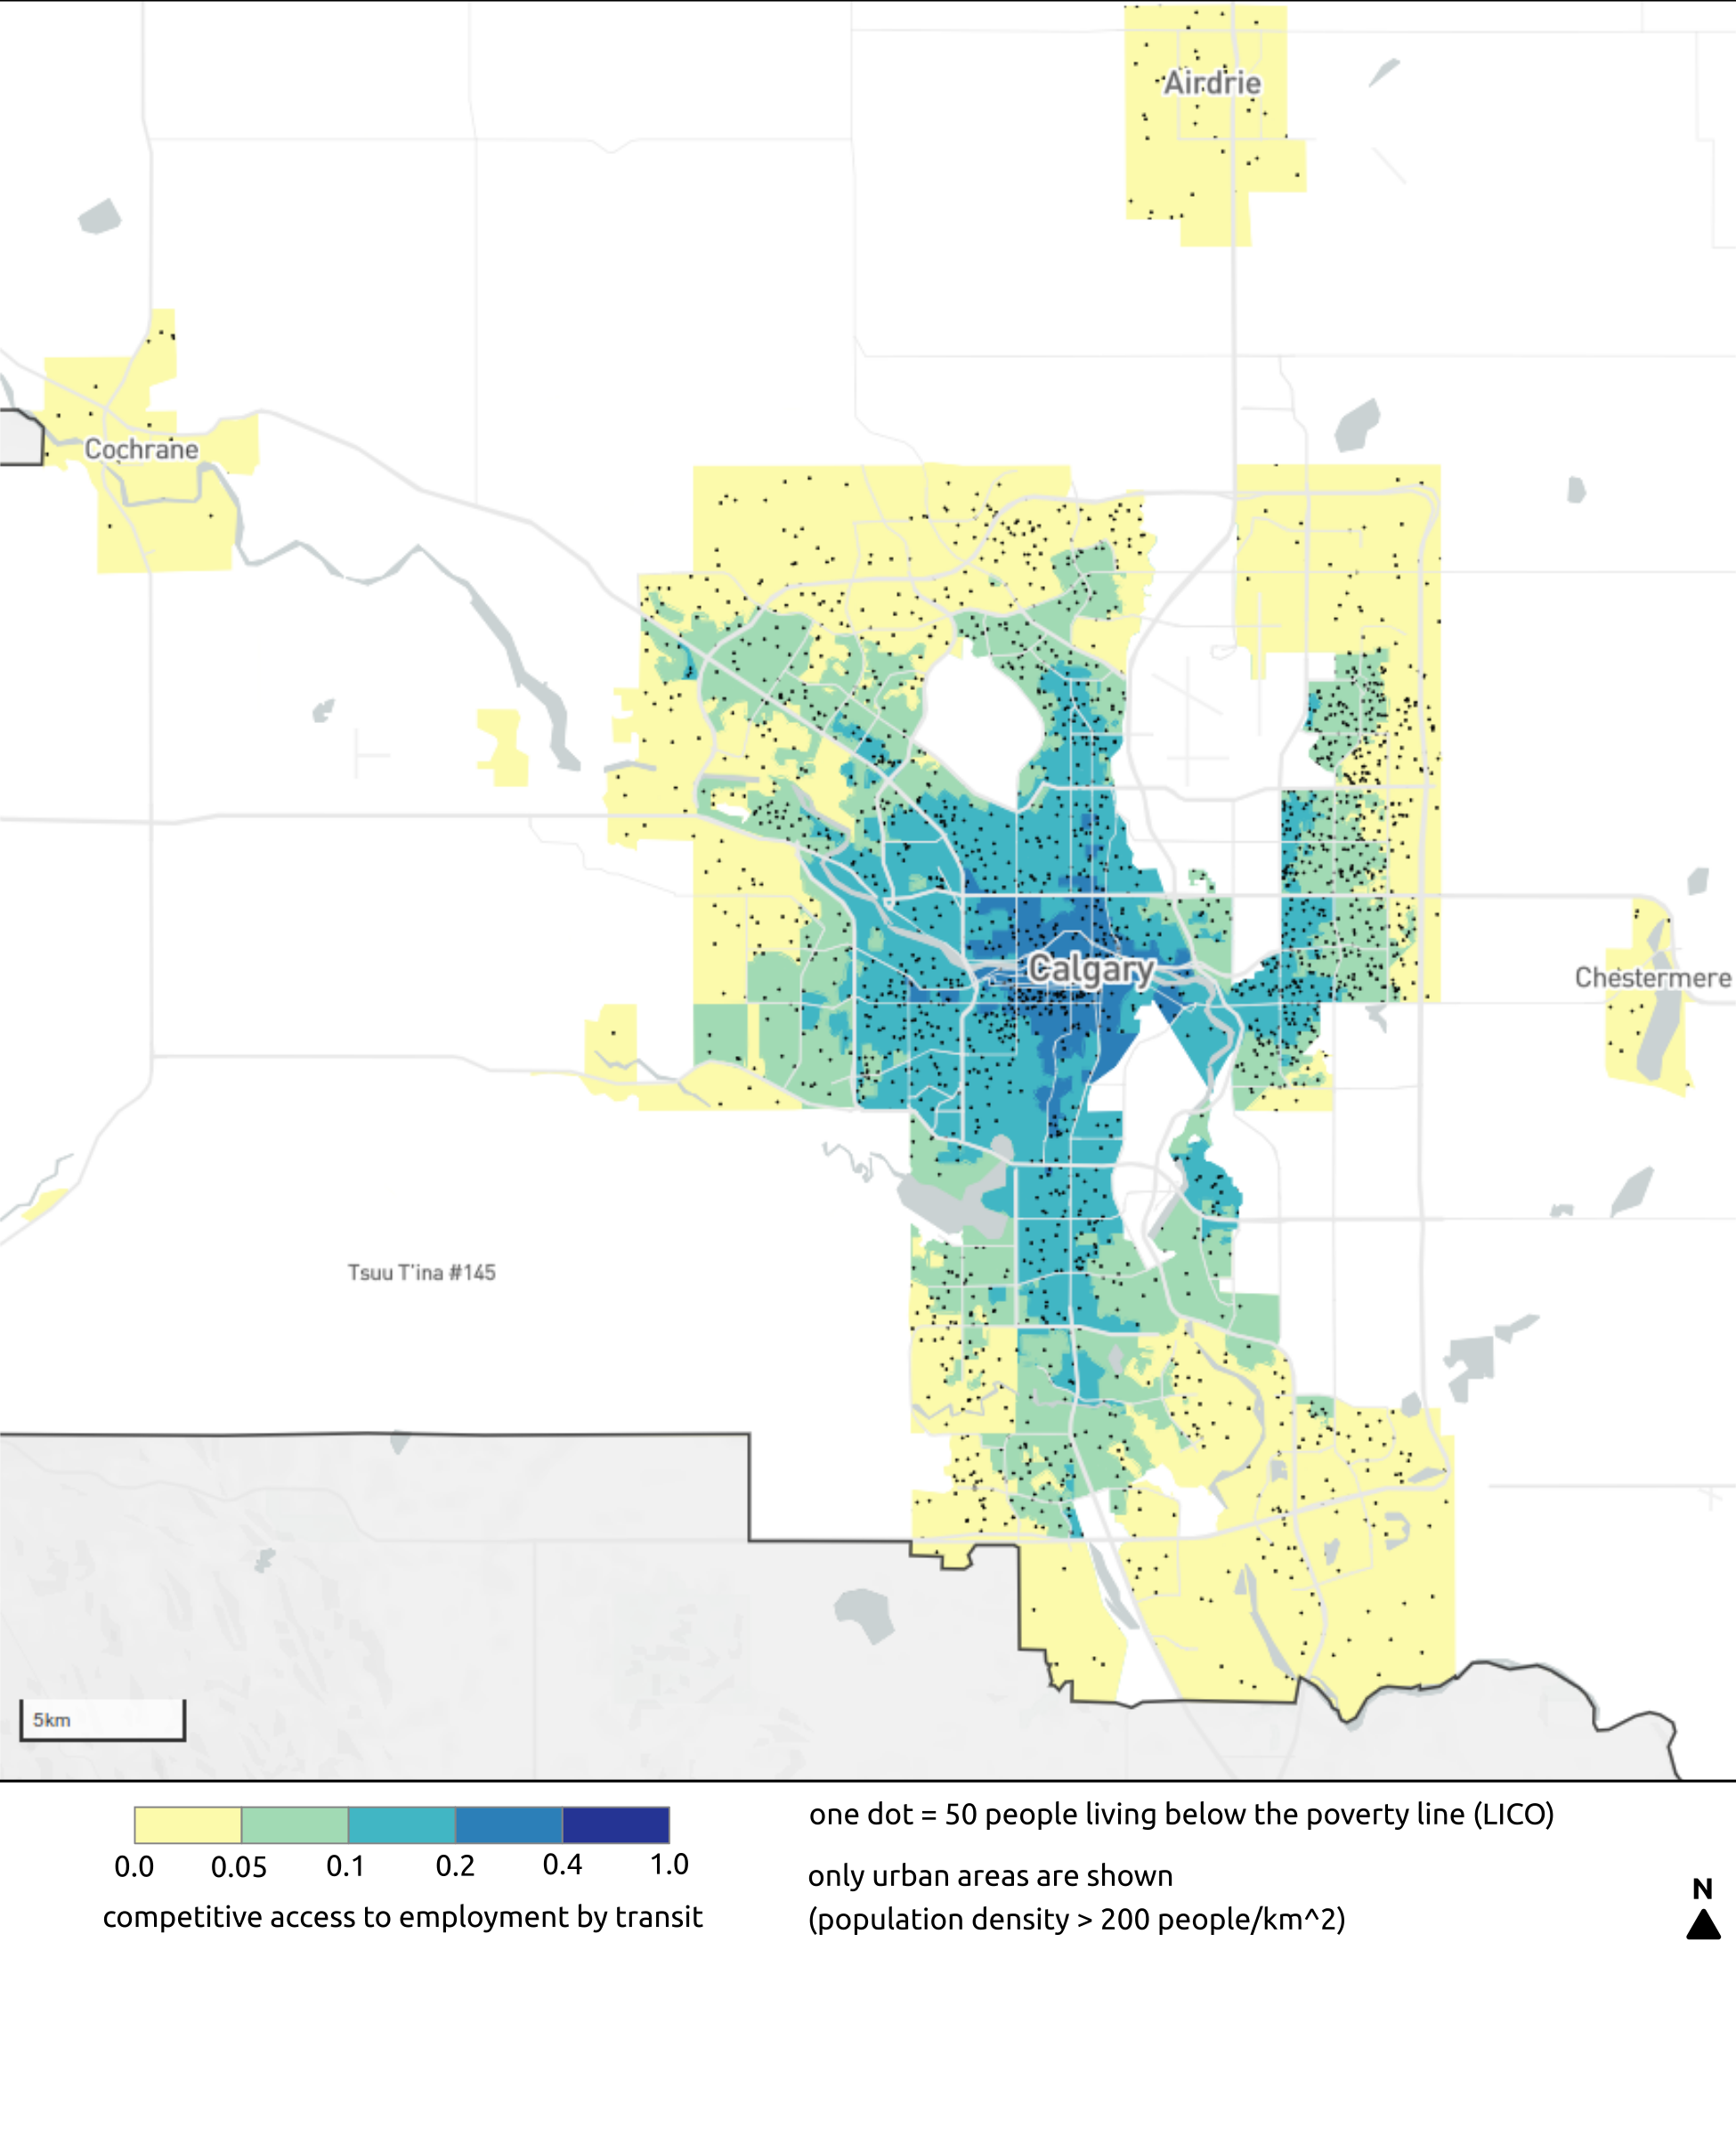
\includegraphics[width=6.5in]{figures/appendix_maps/a_cgy.png}}
	\vspace{2mm}
\end{figure}

\begin{figure}[H]
	\caption{Map of Edmonton showing transit access to employment and low income households} 
	\label{a_van}
	\centerline{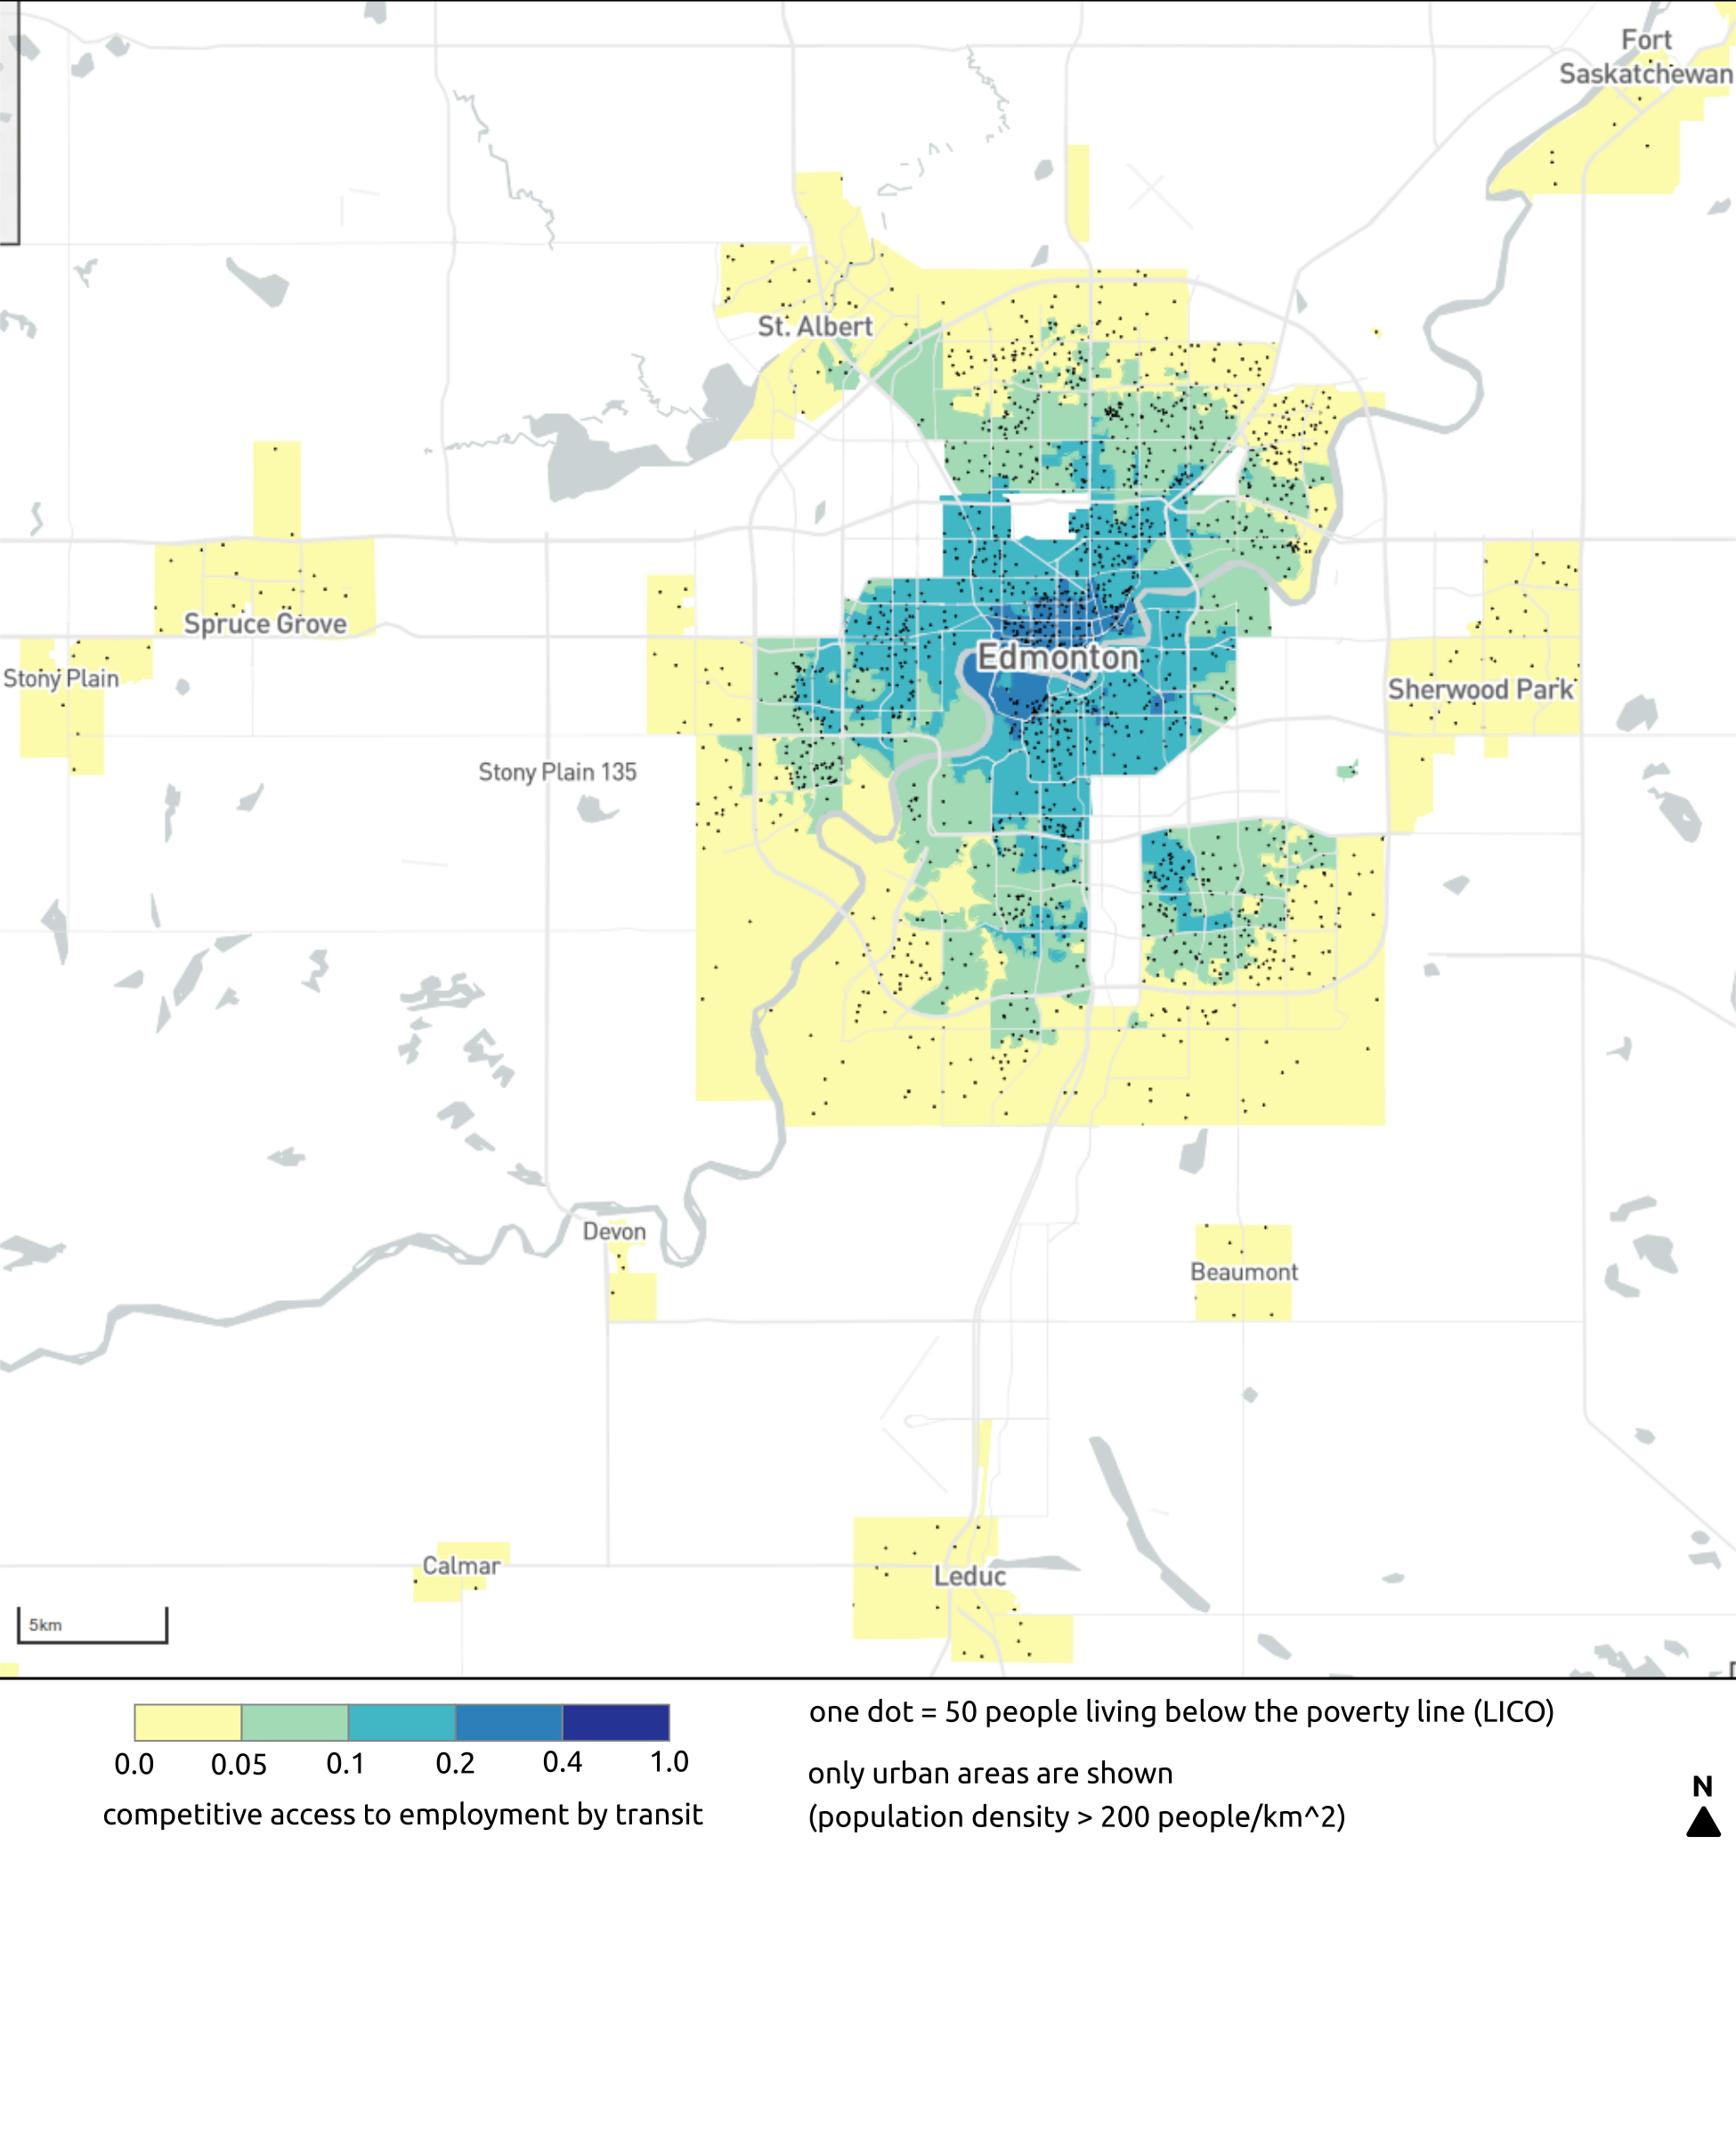
\includegraphics[width=6.5in]{figures/appendix_maps/a_edm.png}}
	\vspace{2mm}
\end{figure}

\begin{figure}[H]
	\caption{Maps of Vancouver showing transit access to employment and low income households} 
	\label{a_van}
	\centerline{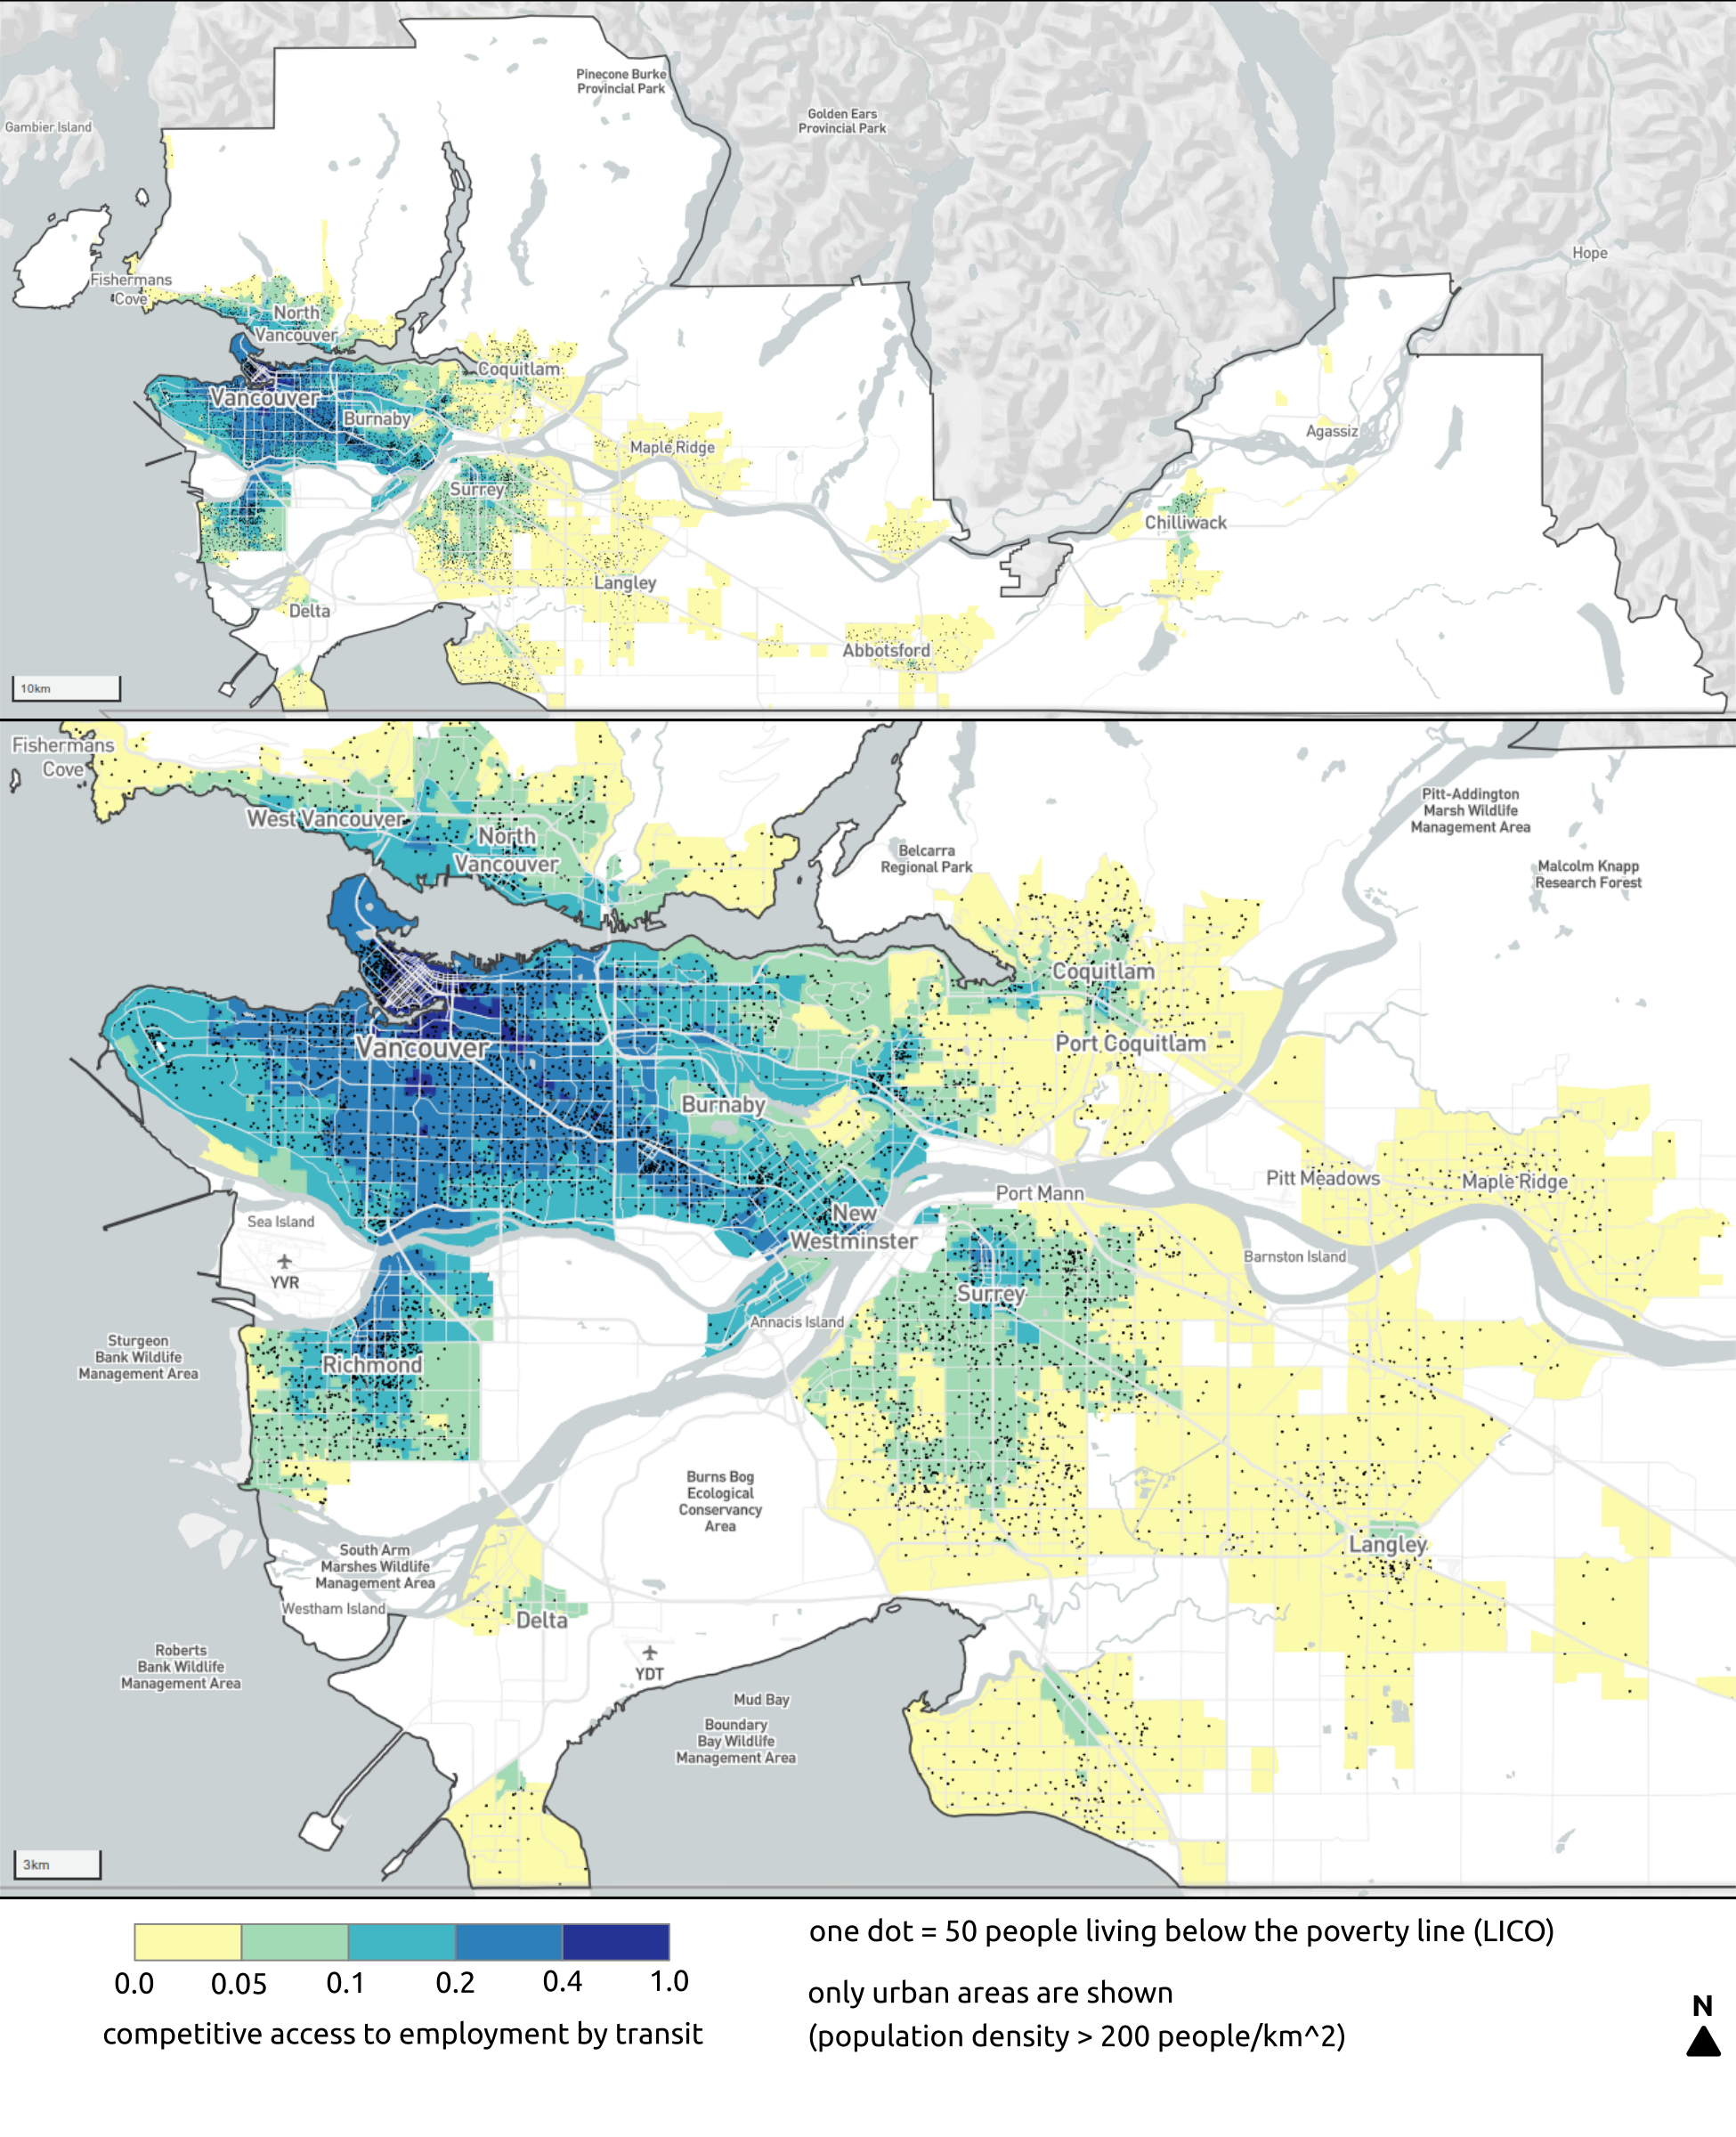
\includegraphics[width=6.5in]{figures/appendix_maps/a_van.png}}
	\vspace{2mm}
\end{figure}

\subsection{Maps of the cluster analysis of areas at high risk of transport poverty}

\begin{figure}[H]
	\caption{Map of the location of cluster groups for Quebec City} 
	\label{C_que}
	\centerline{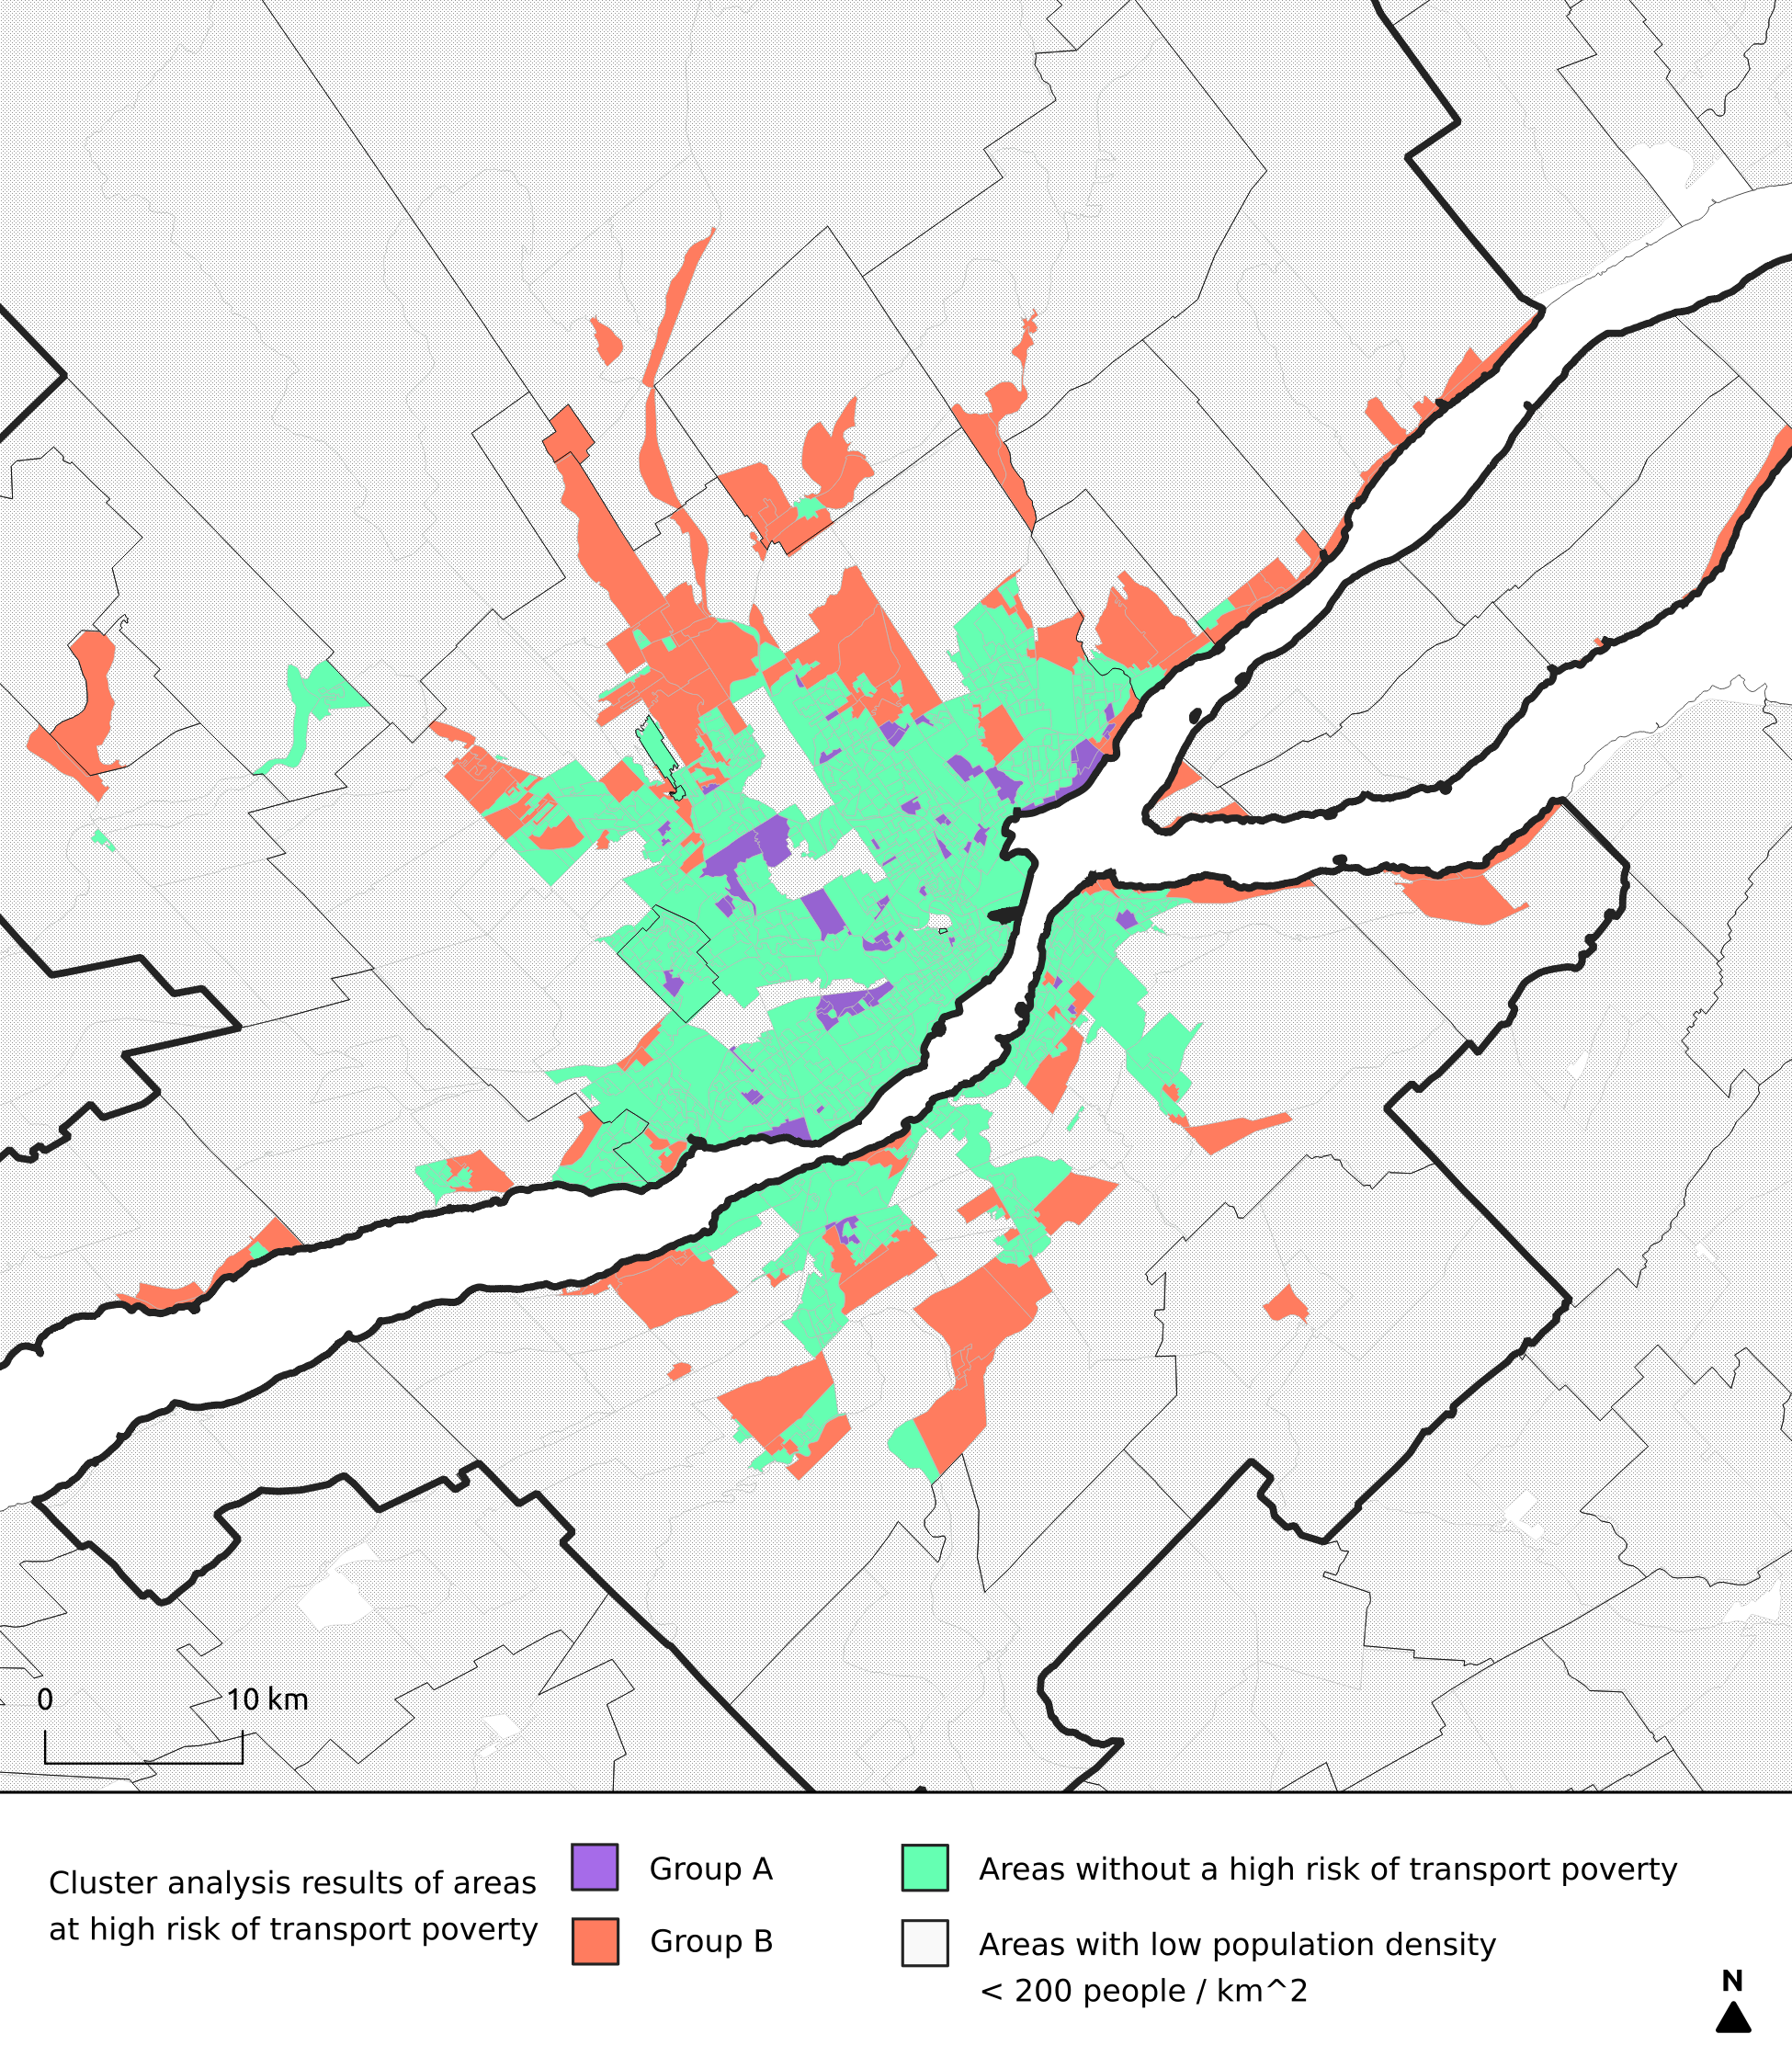
\includegraphics[width=6.5in]{figures/cluster_maps/C_que}}
	\vspace{2mm}
\end{figure}

\begin{figure}[H]
	\caption{Map of the location of cluster groups for Montreal} 
	\label{C_mtl}
	\centerline{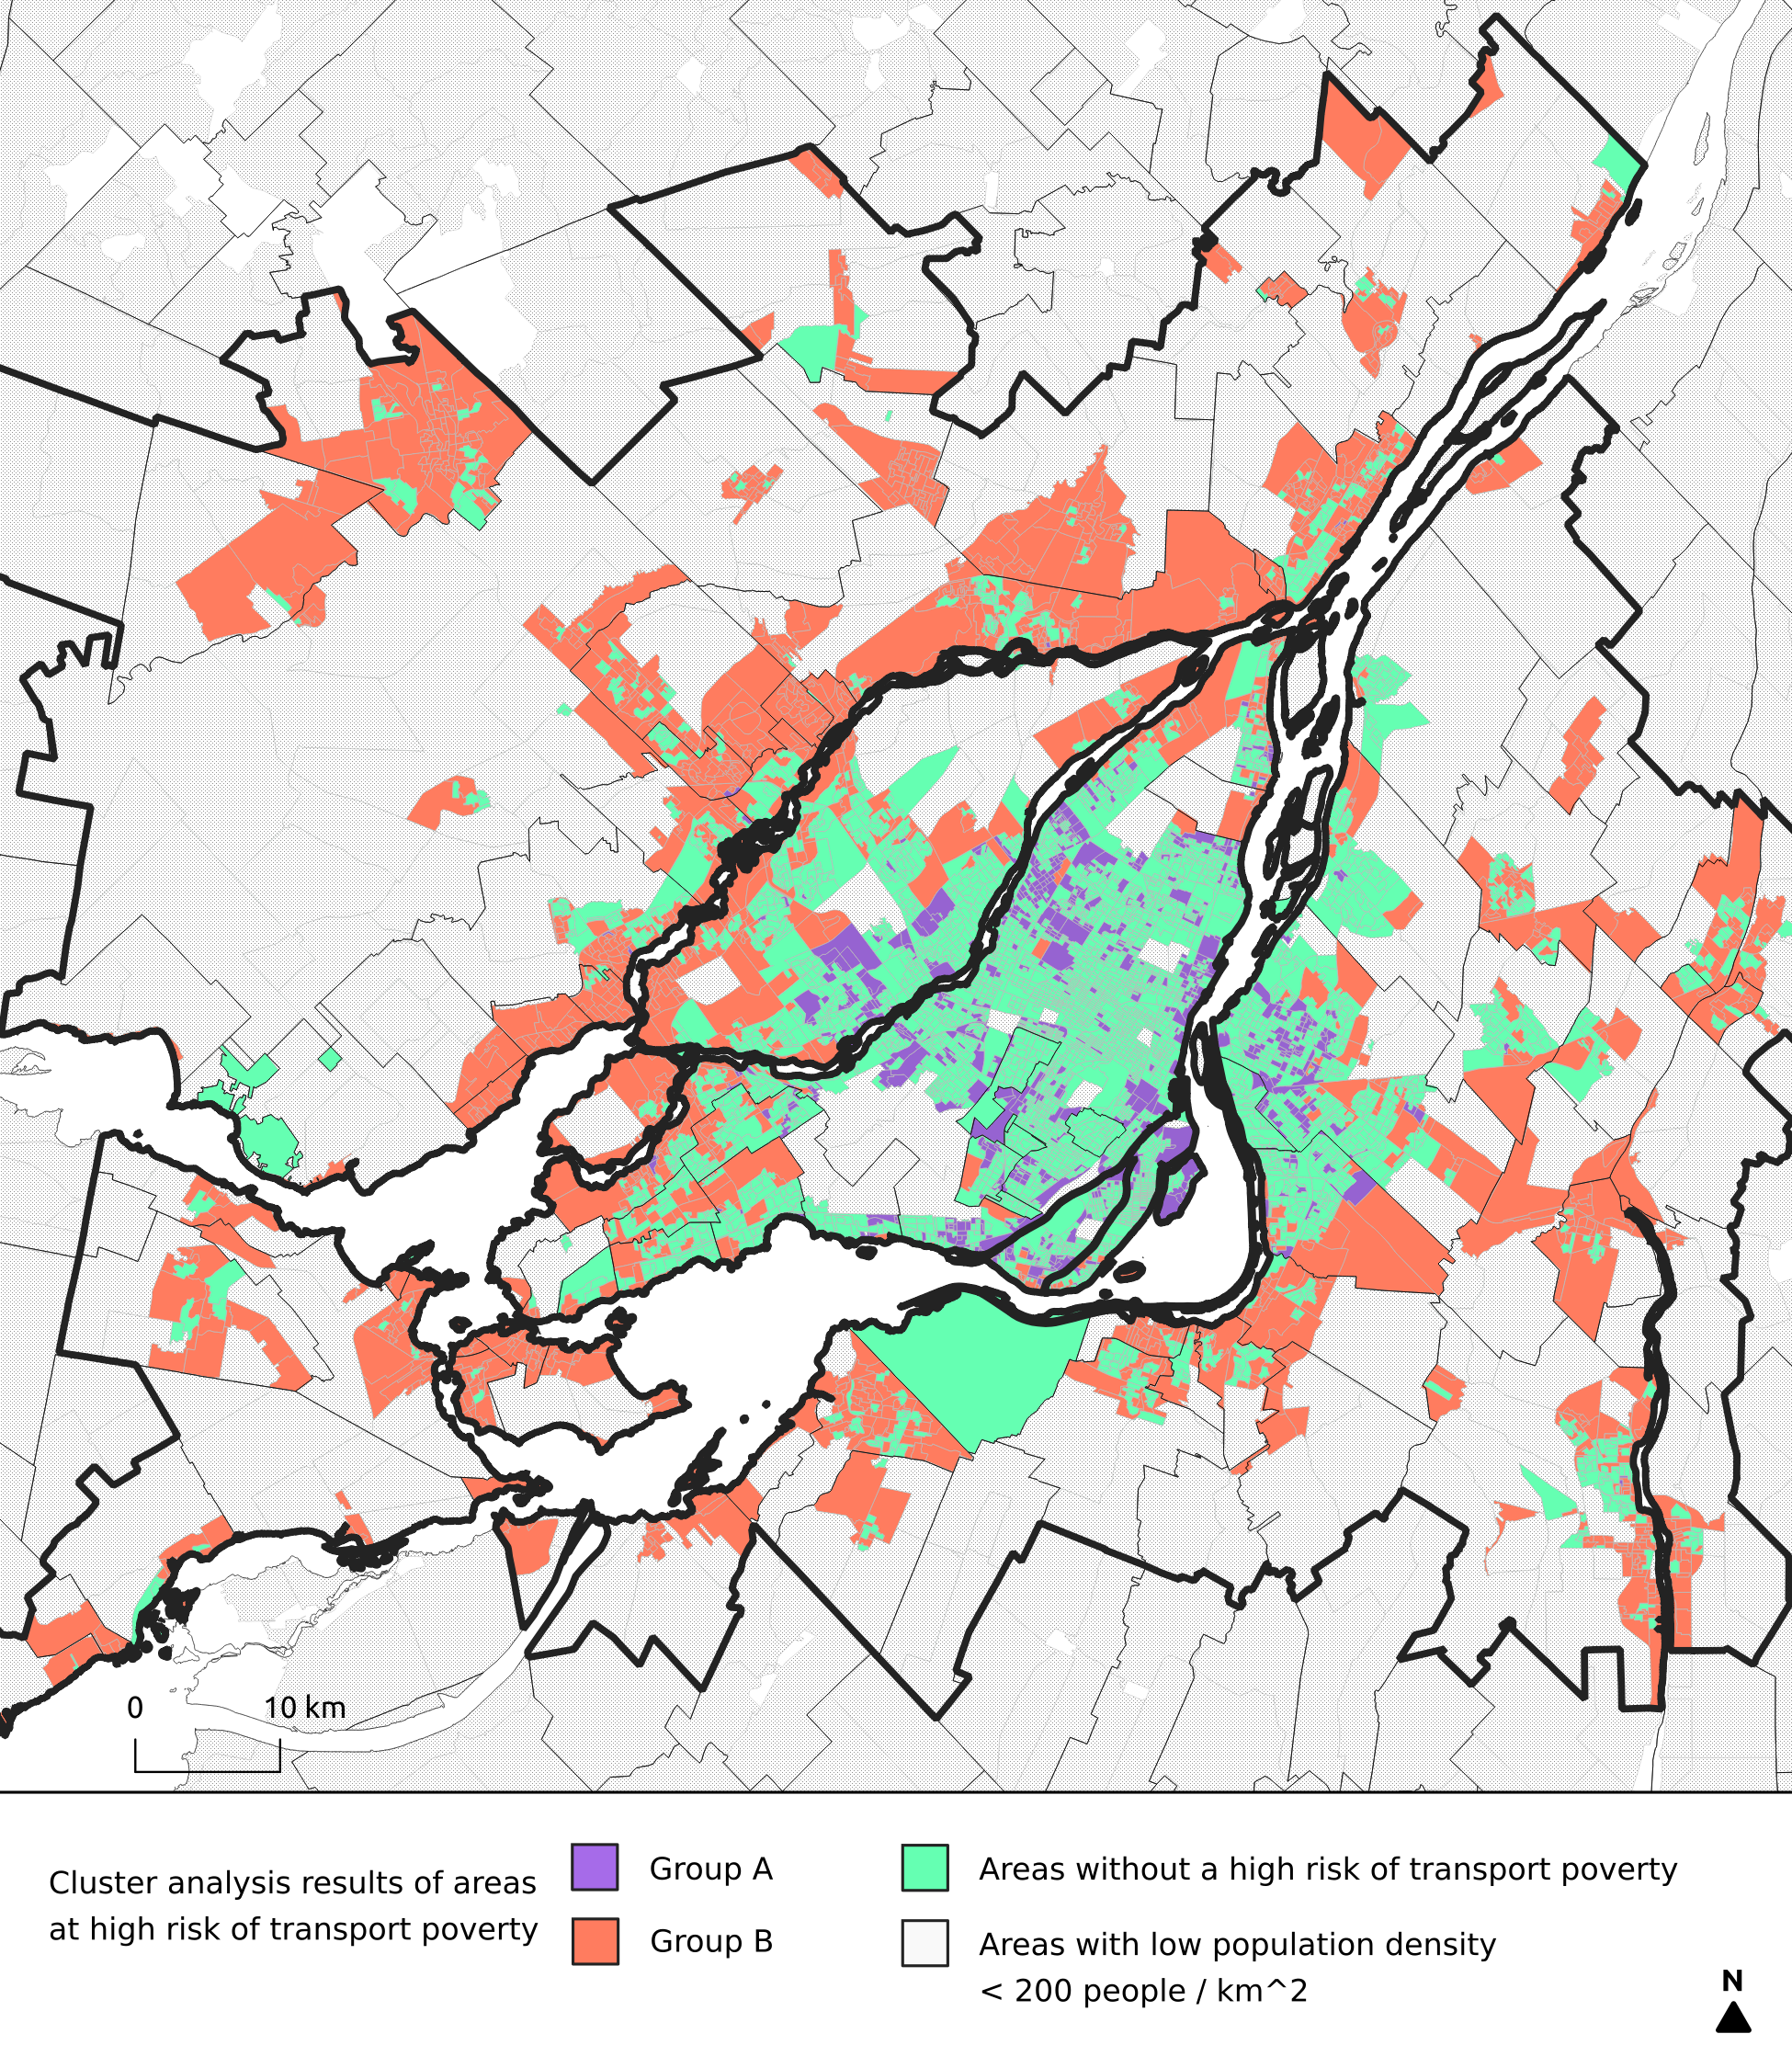
\includegraphics[width=6.5in]{figures/cluster_maps/C_mtl}}
	\vspace{2mm}
\end{figure}

\begin{figure}[H]
	\caption{Map of the location of cluster groups for Ottawa} 
	\label{C_ott}
	\centerline{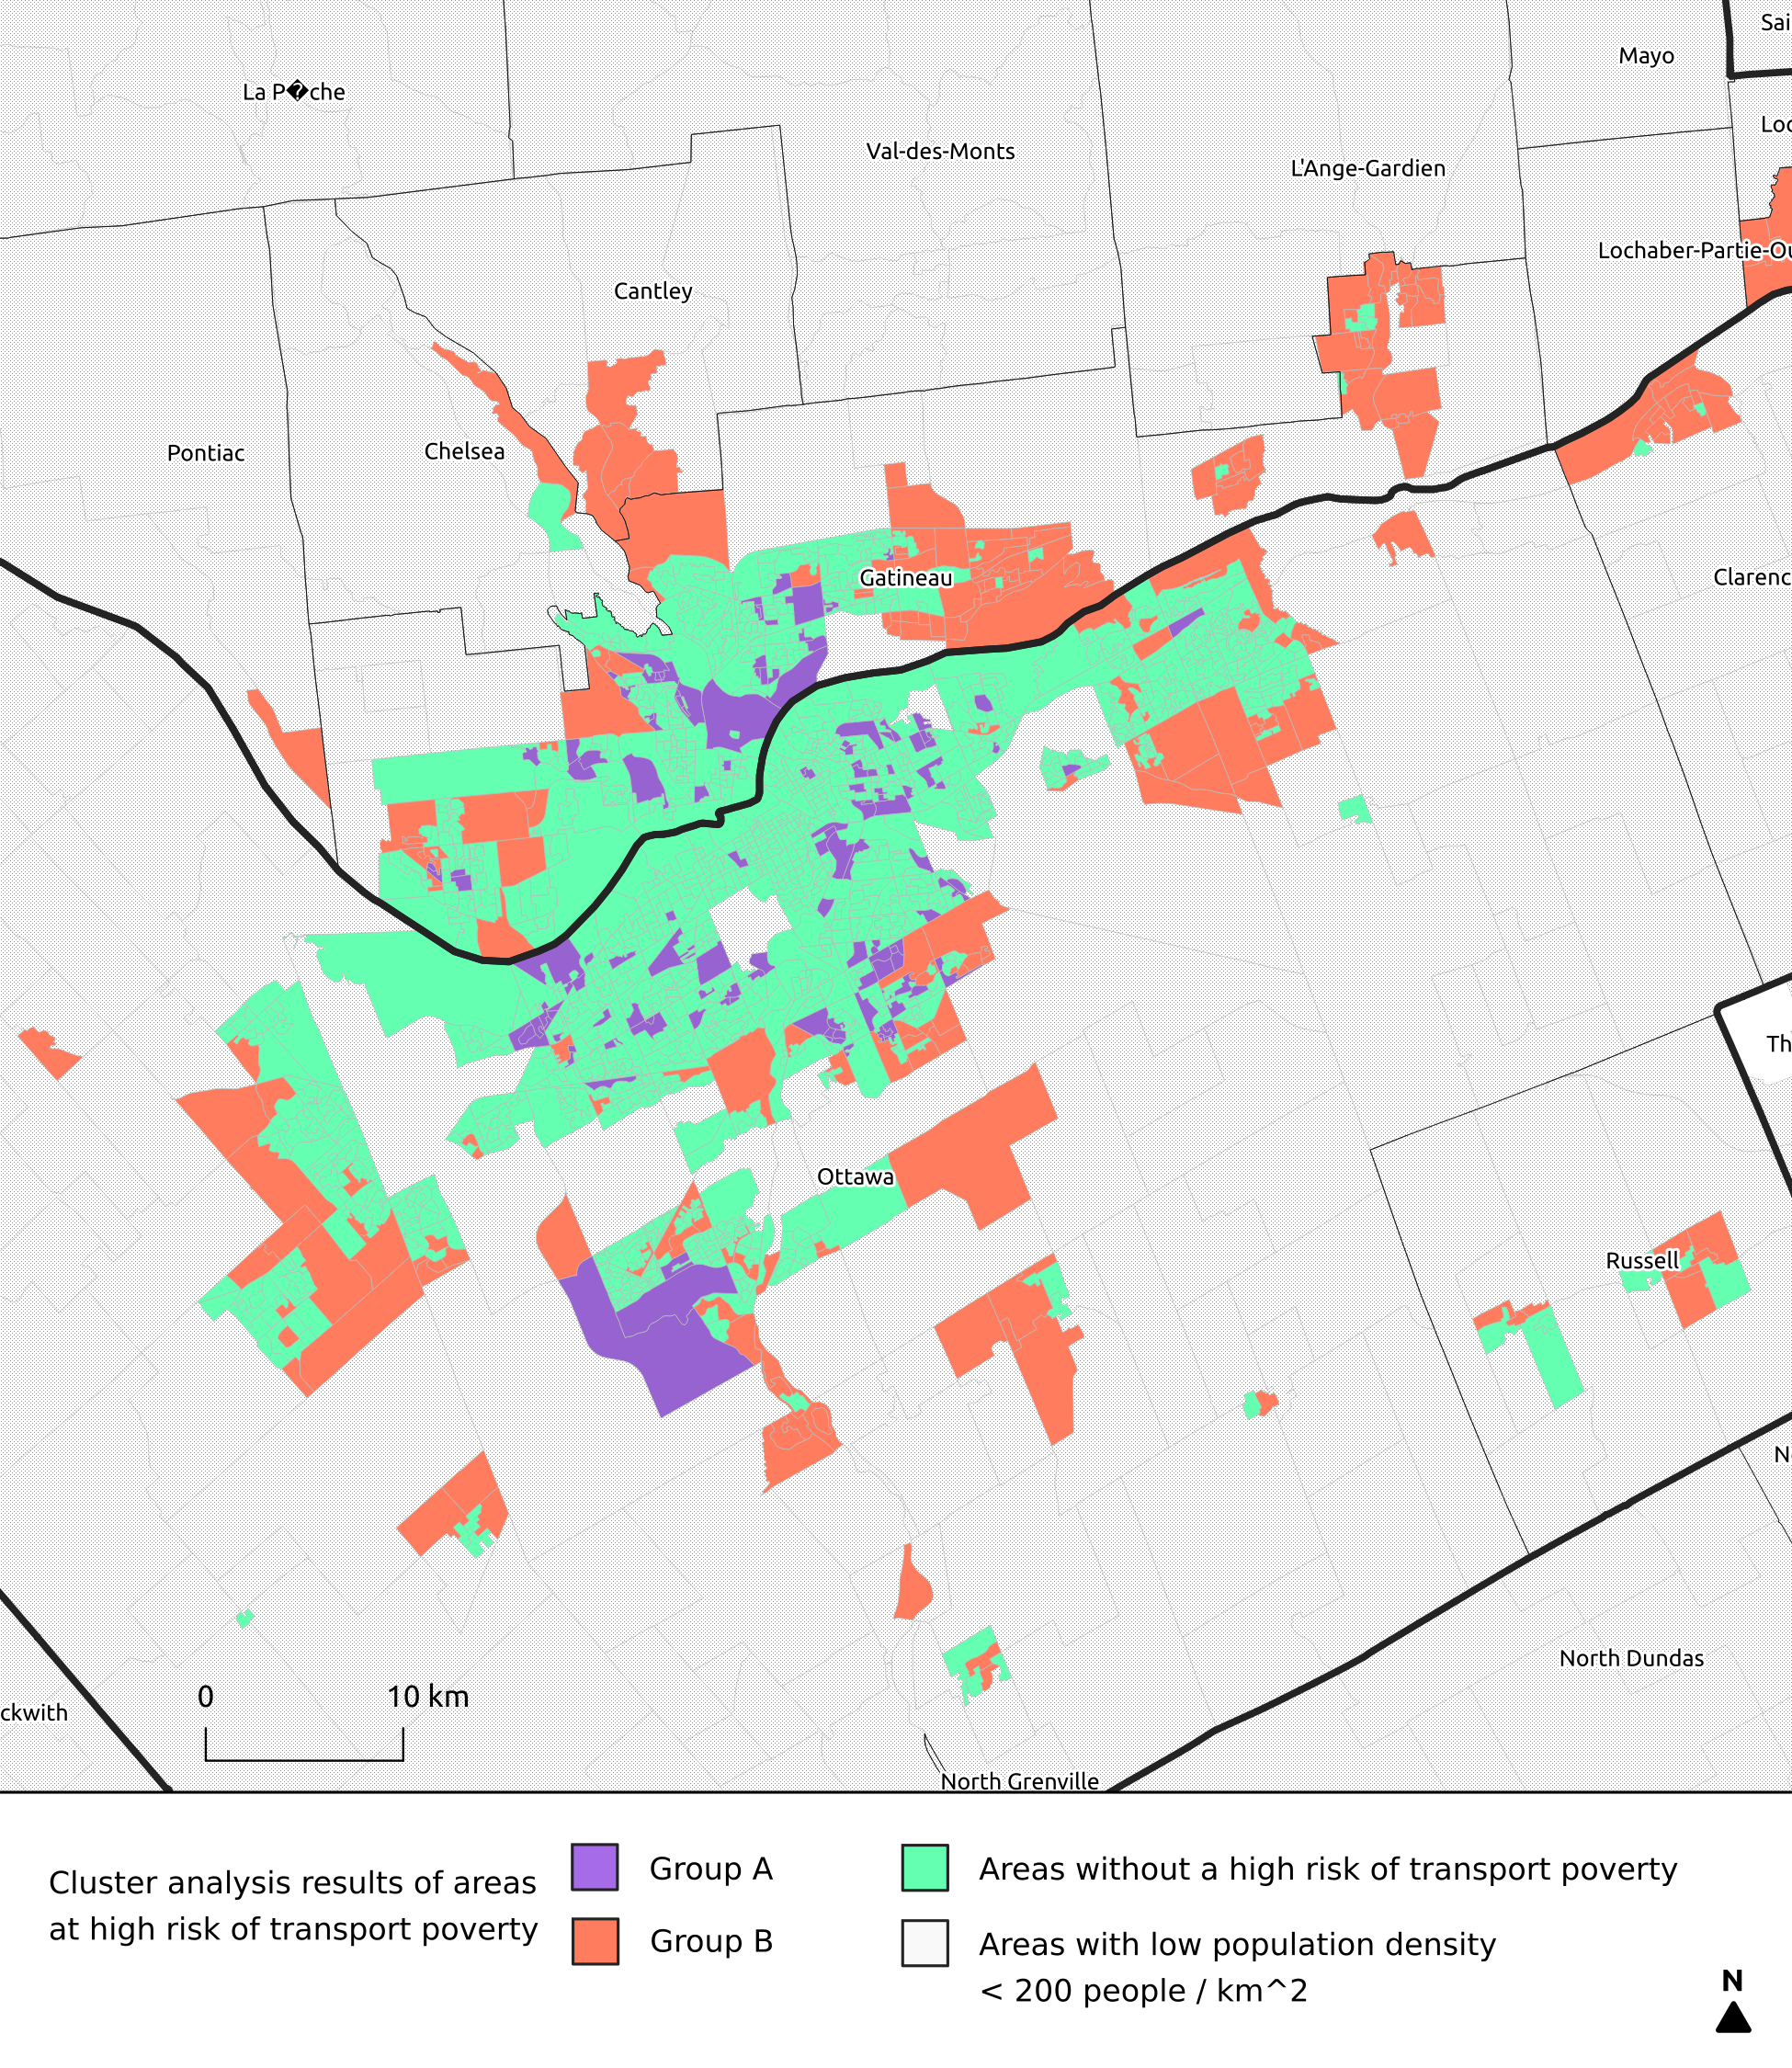
\includegraphics[width=6.5in]{figures/cluster_maps/C_ott}}
	\vspace{2mm}
\end{figure}

\begin{figure}[H]
	\caption{Map of the location of cluster groups for Toronto} 
	\label{C_tor}
	\centerline{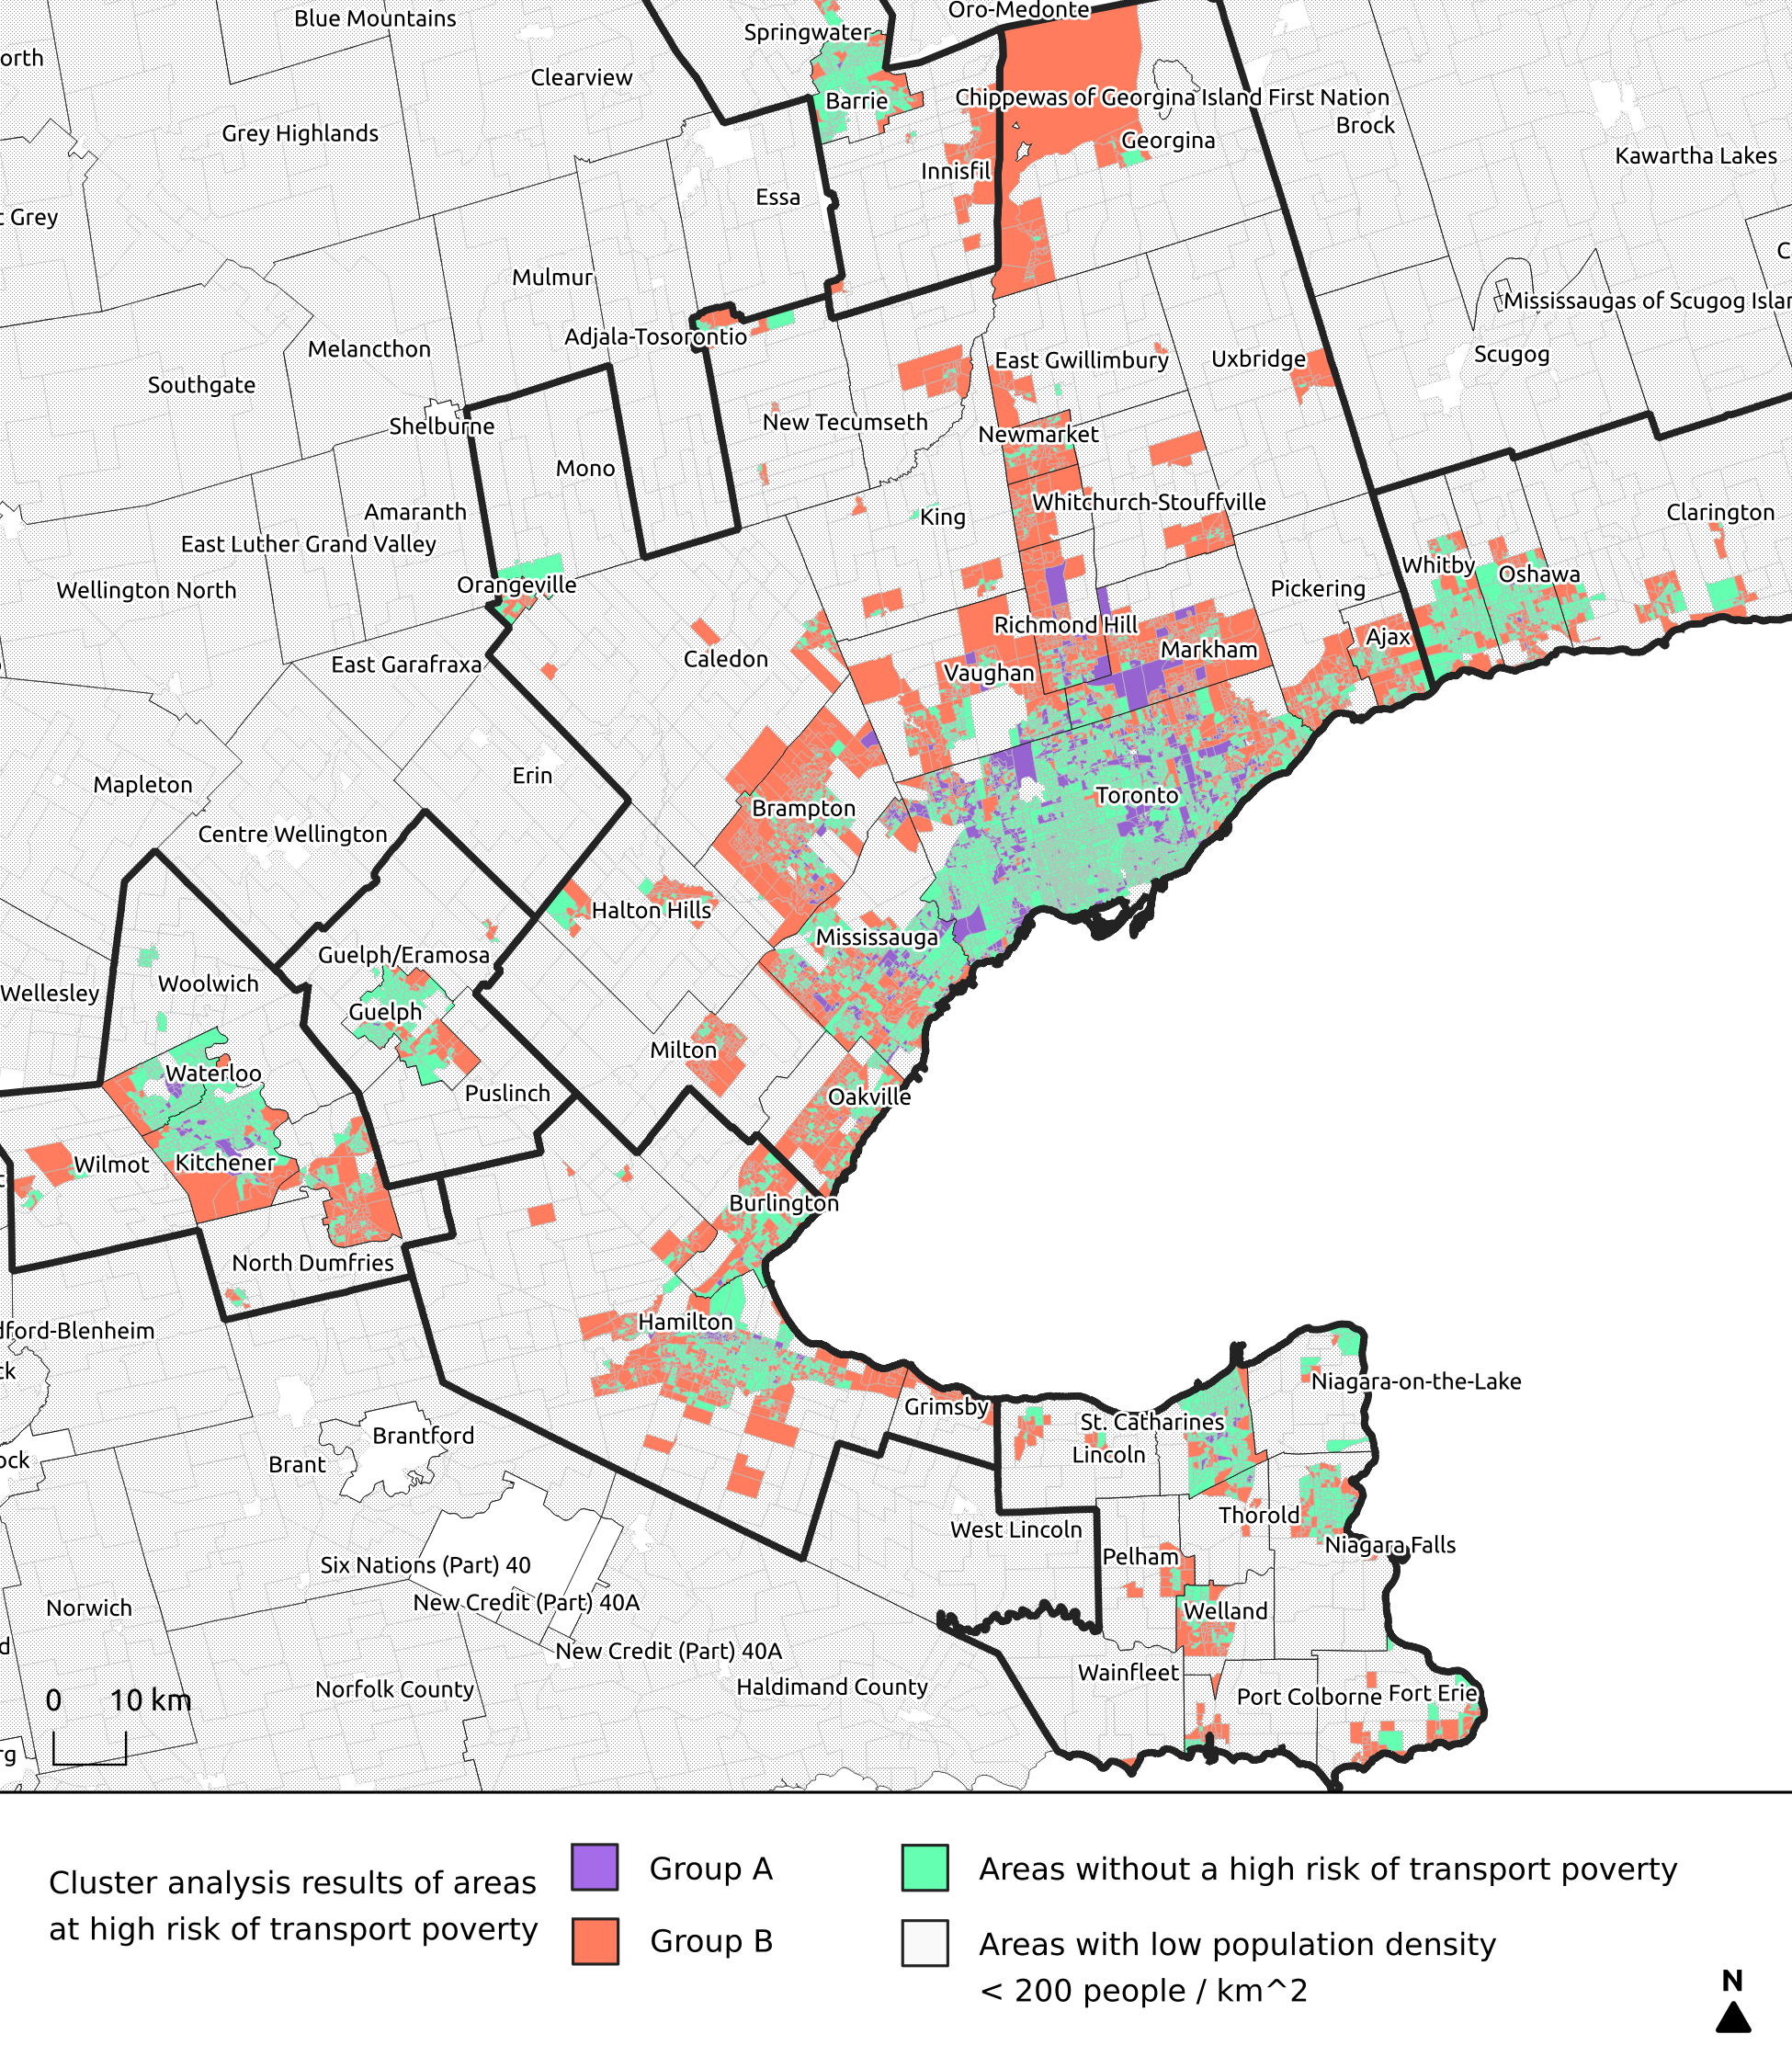
\includegraphics[width=6.5in]{figures/cluster_maps/C_tor}}
	\vspace{2mm}
\end{figure}

\begin{figure}[H]
	\caption{Map of the location of cluster groups for Winnipeg} 
	\label{C_wpg}
	\centerline{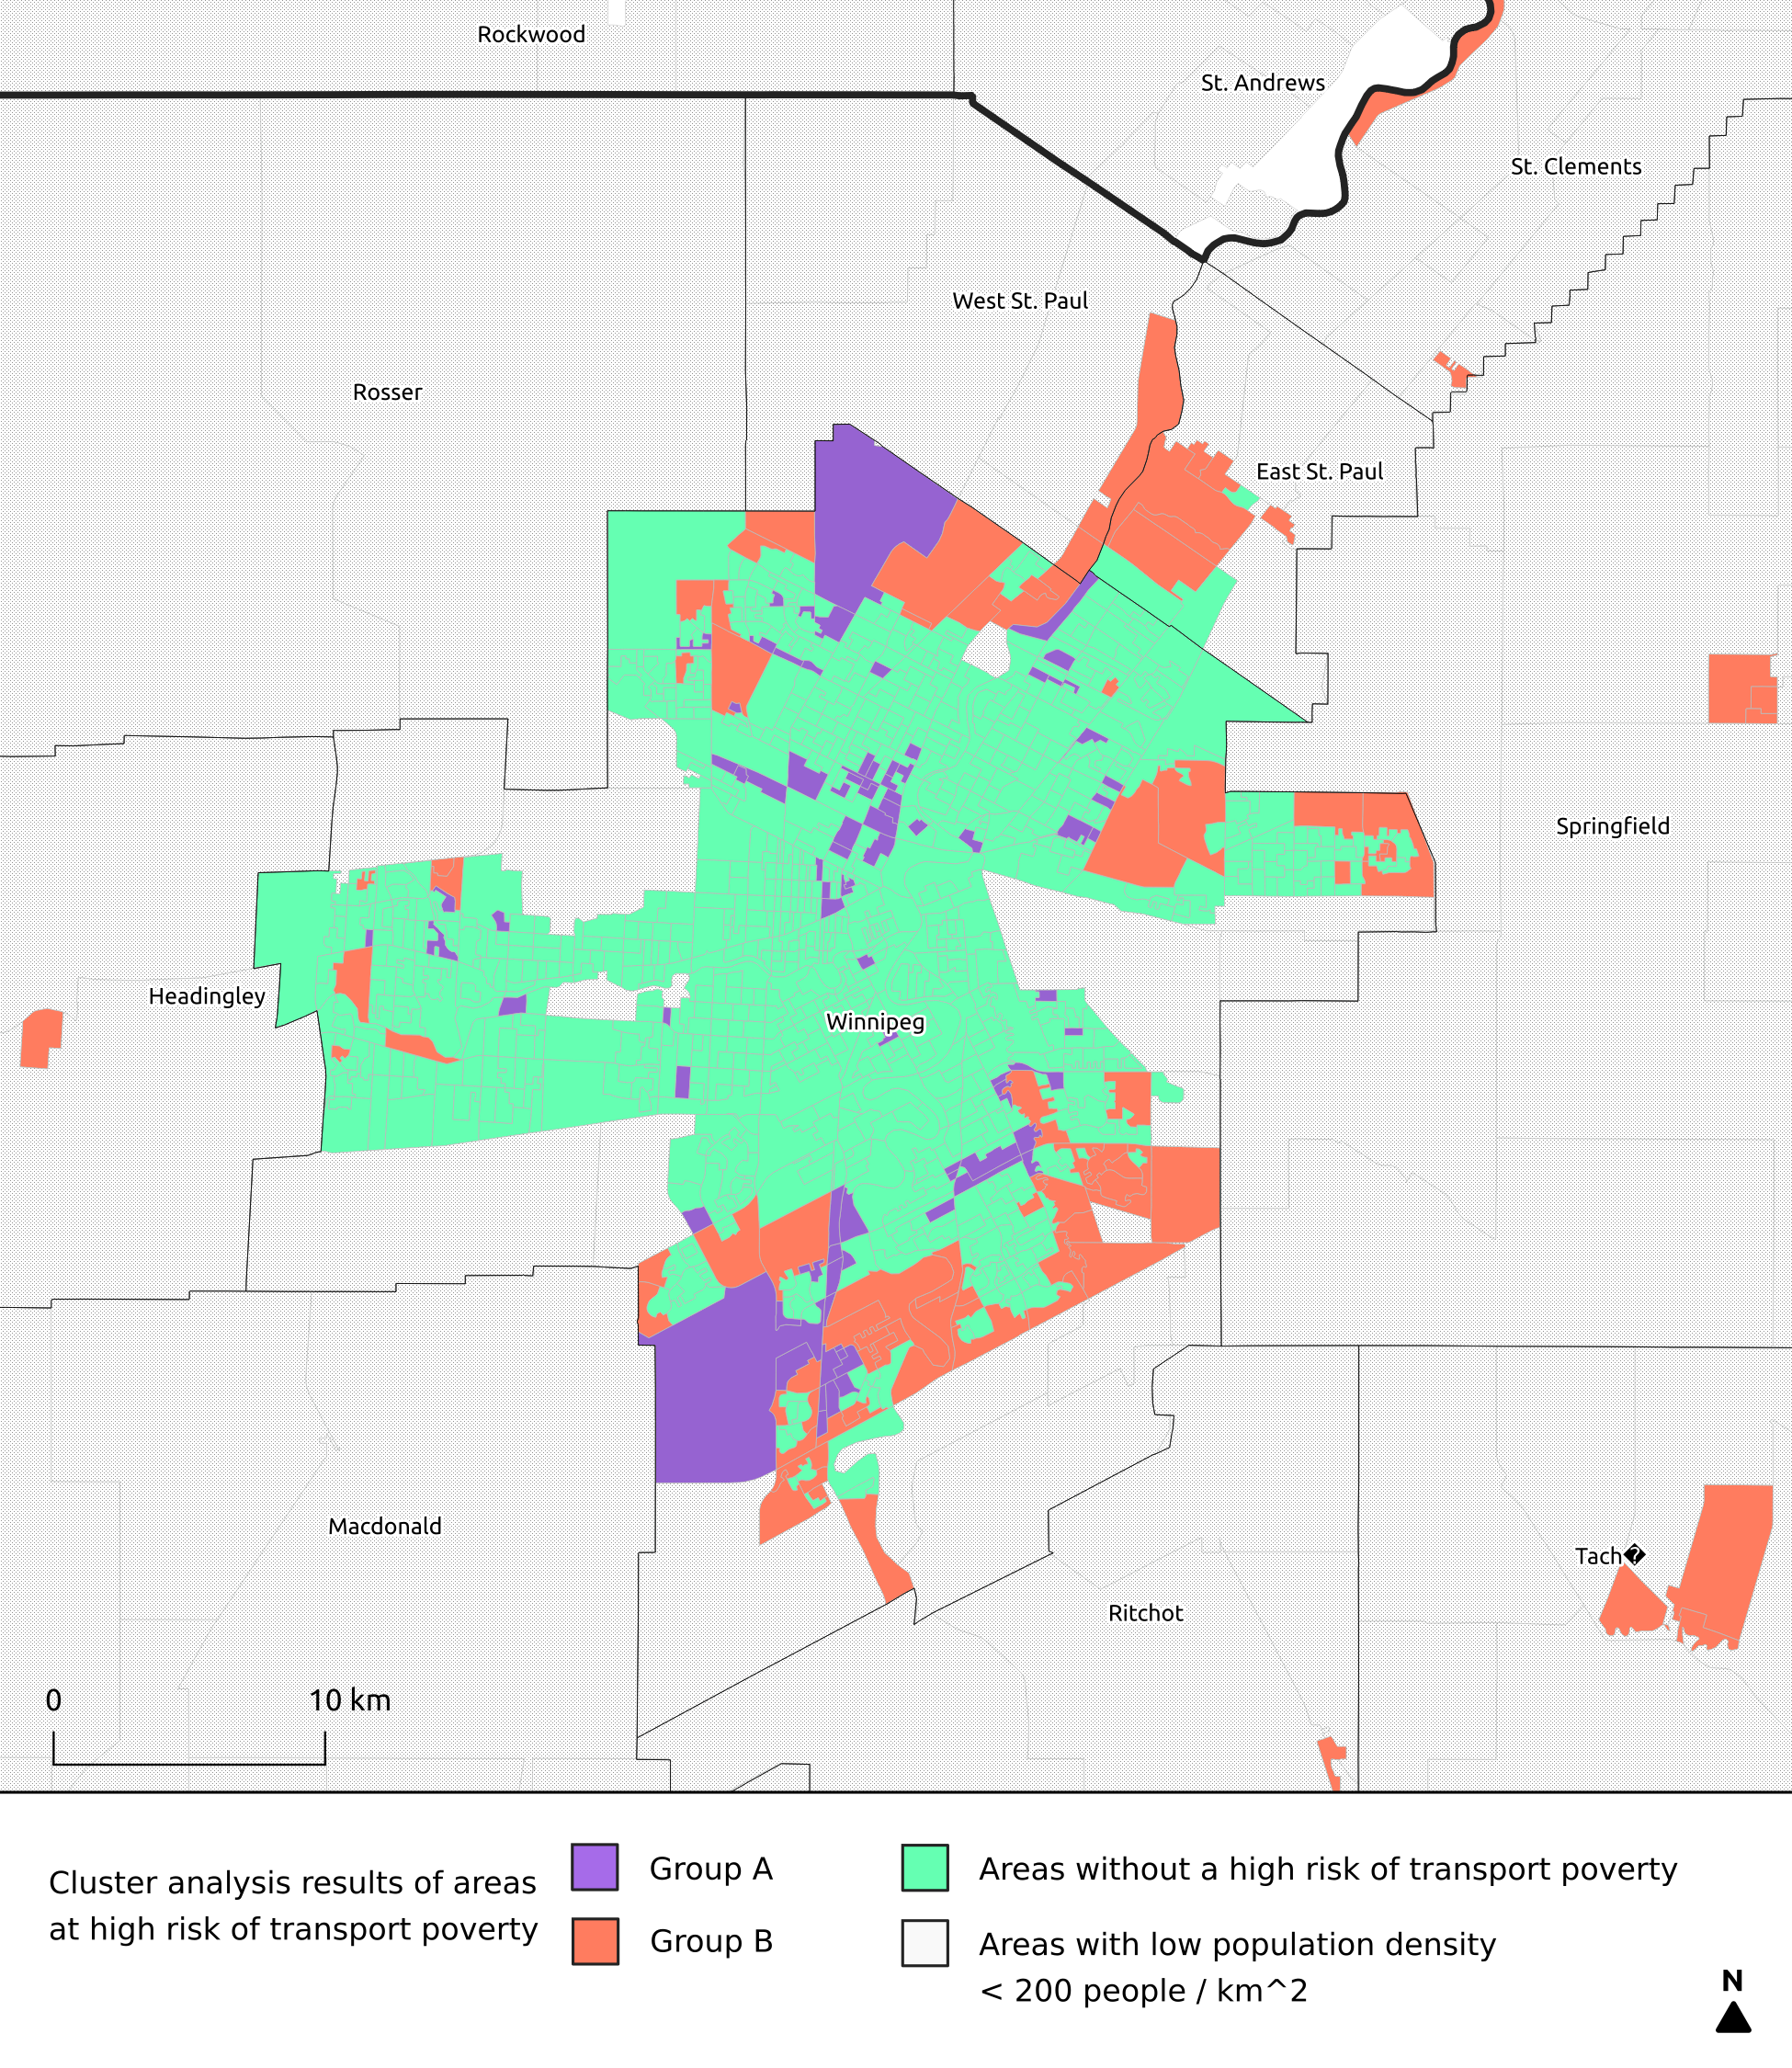
\includegraphics[width=6.5in]{figures/cluster_maps/C_wpg}}
	\vspace{2mm}
\end{figure}

\begin{figure}[H]
	\caption{Map of the location of cluster groups for Calgary} 
	\label{C_cgy}
	\centerline{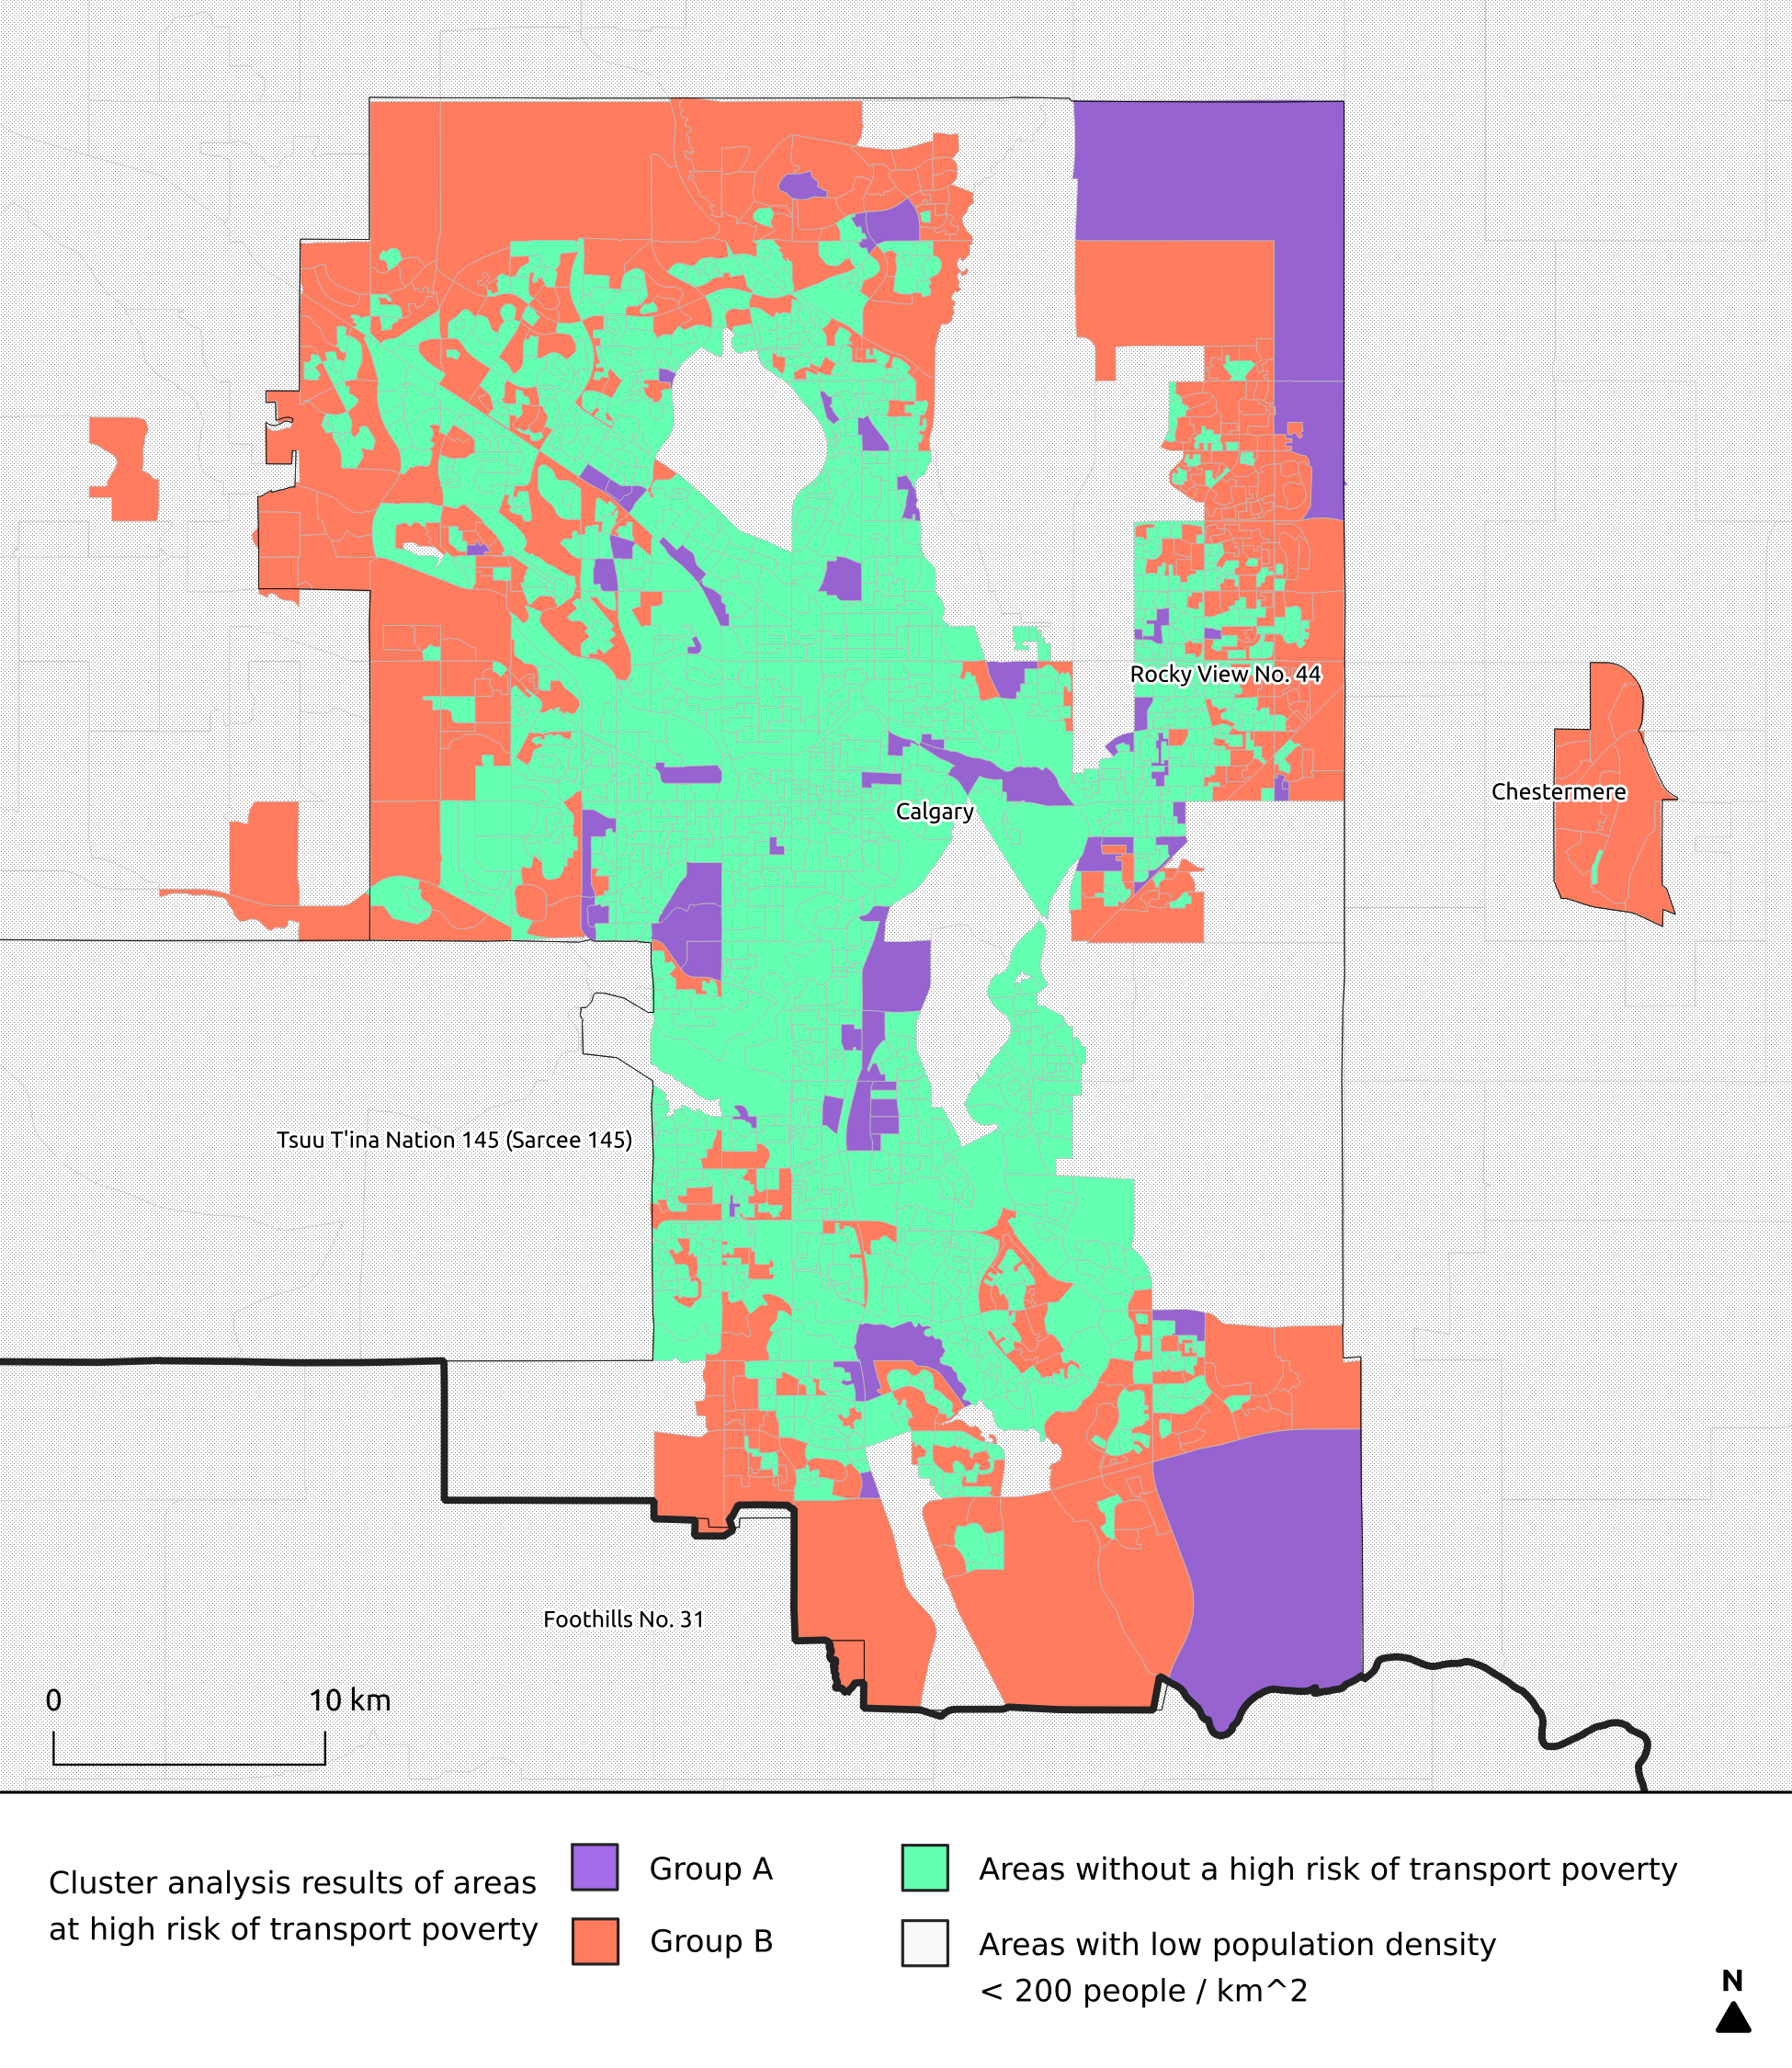
\includegraphics[width=6.5in]{figures/cluster_maps/C_cgy}}
	\vspace{2mm}
\end{figure}

\begin{figure}[H]
	\caption{Map of the location of cluster groups for Edmonton} 
	\label{C_edm}
	\centerline{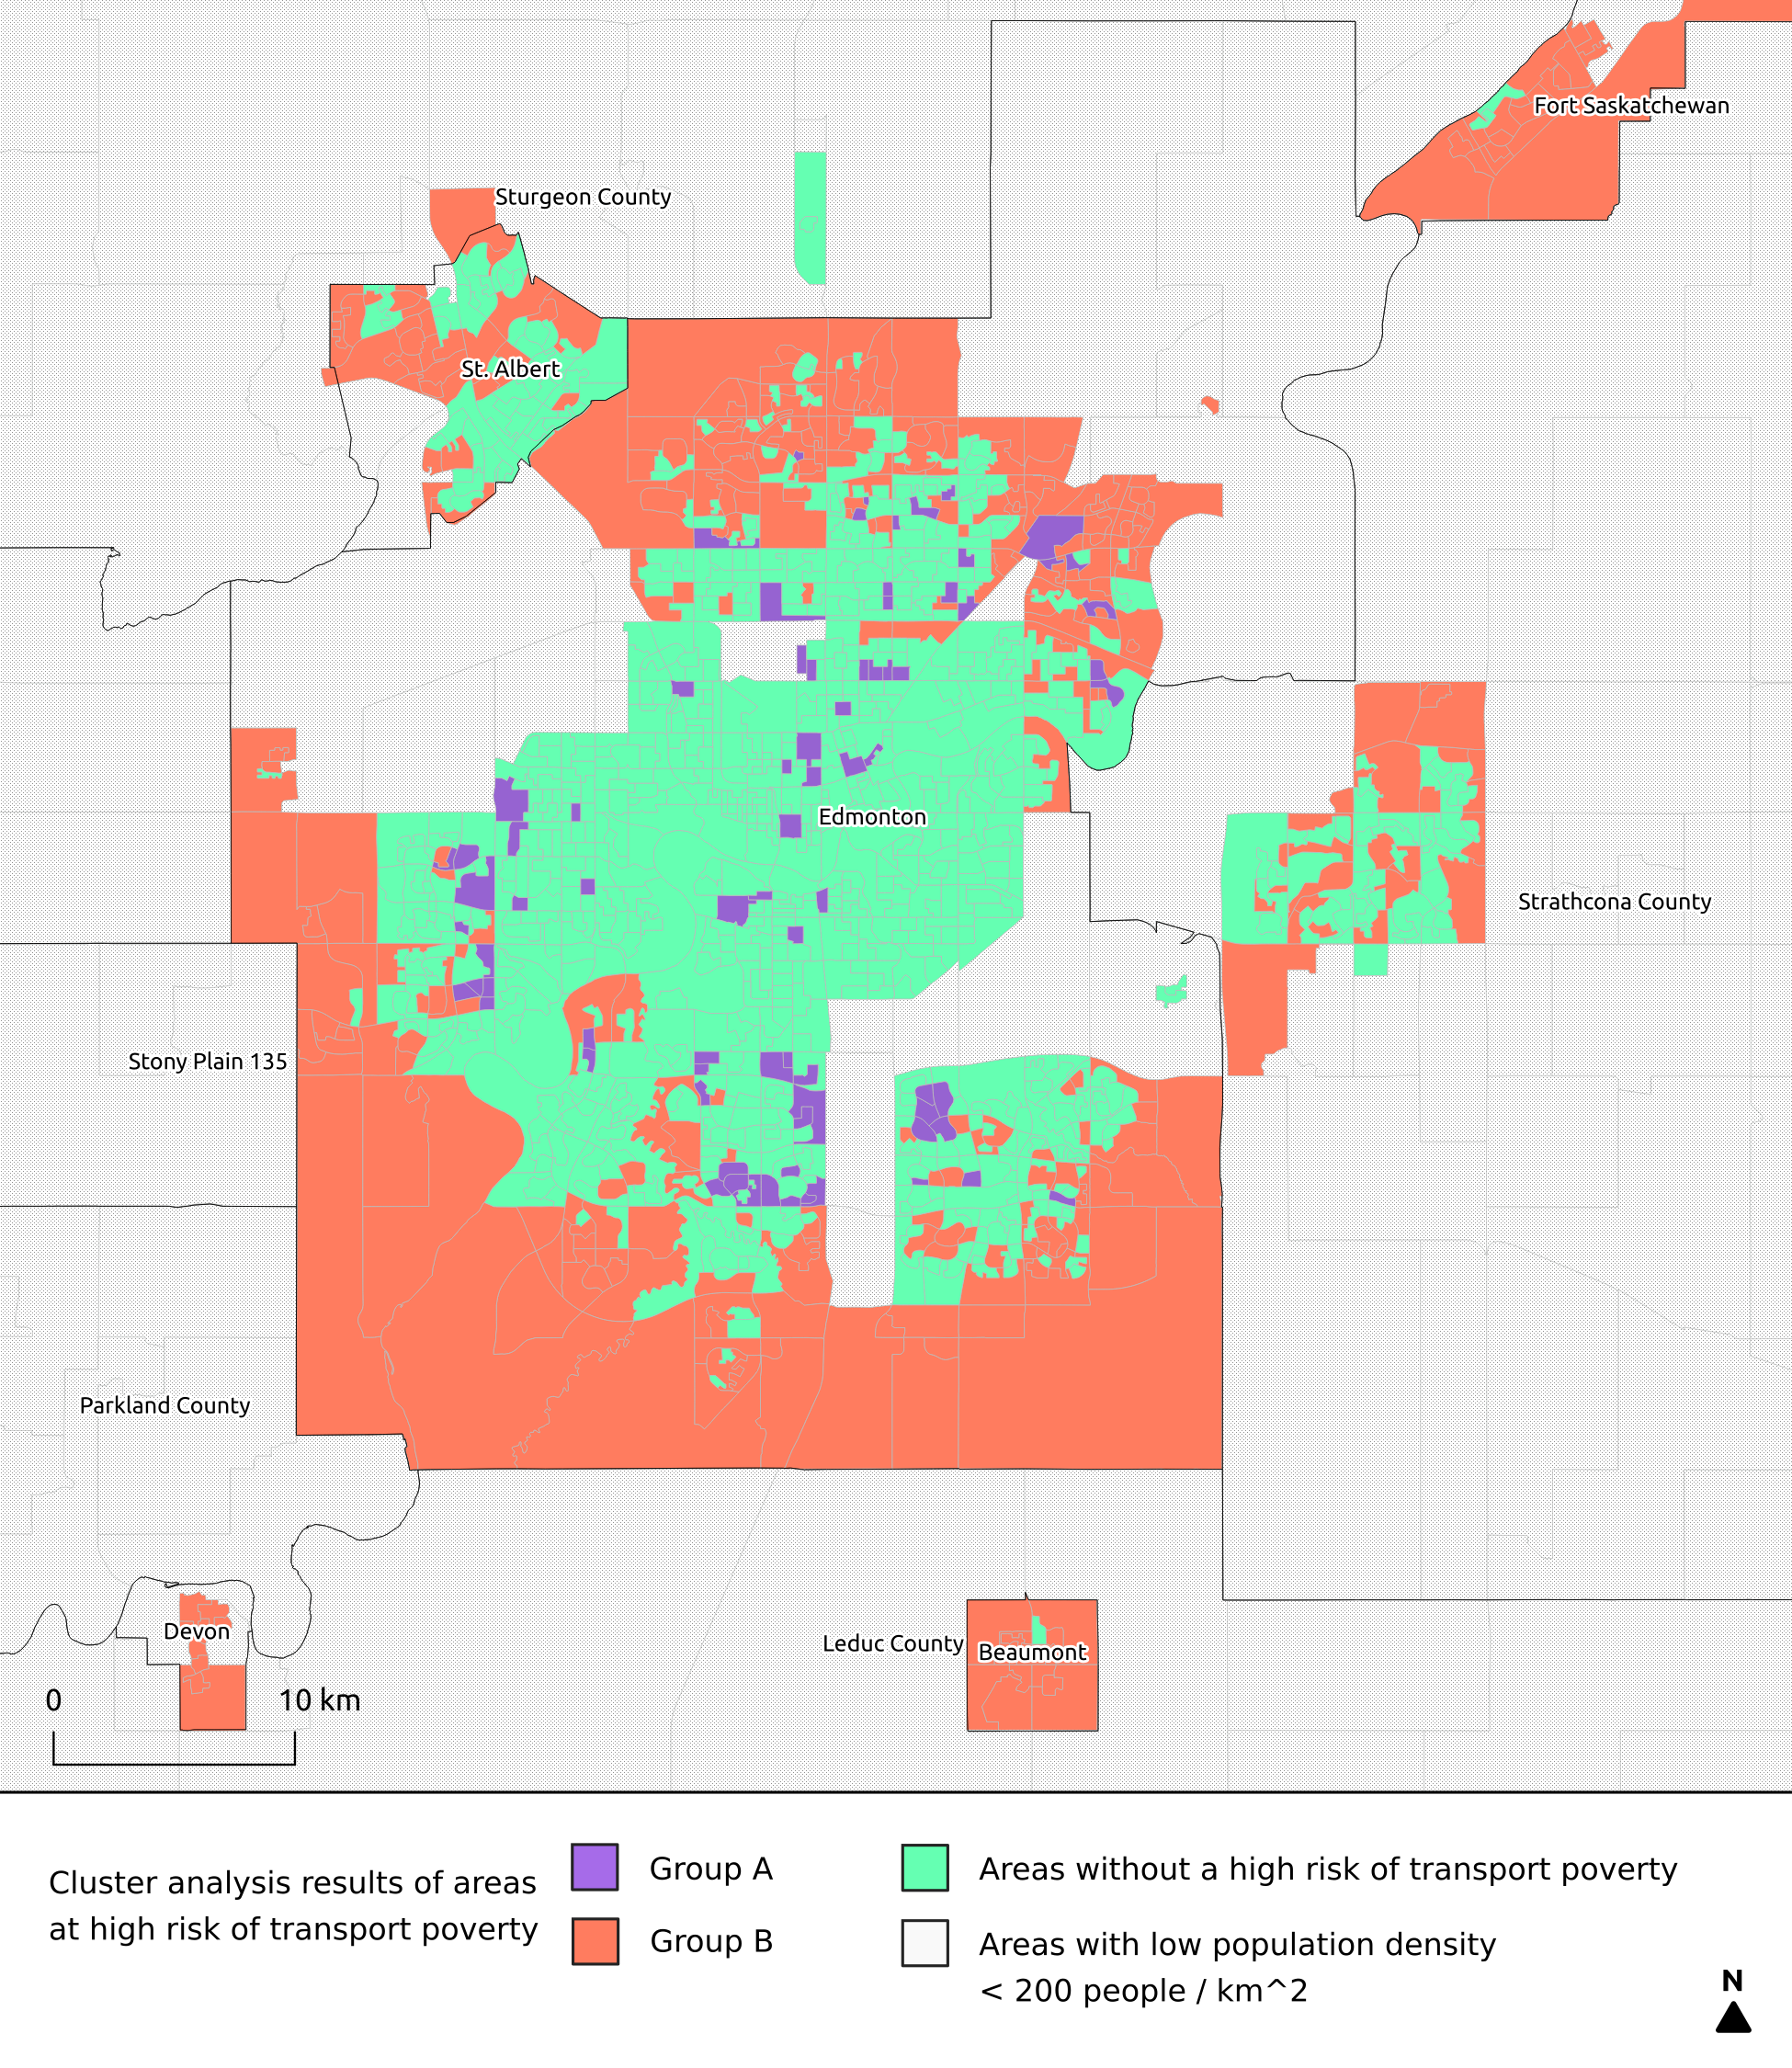
\includegraphics[width=6.5in]{figures/cluster_maps/C_edm}}
	\vspace{2mm}
\end{figure}

\begin{figure}[H]
	\caption{Map of the location of cluster groups for Vancouver} 
	\label{C_van}
	\centerline{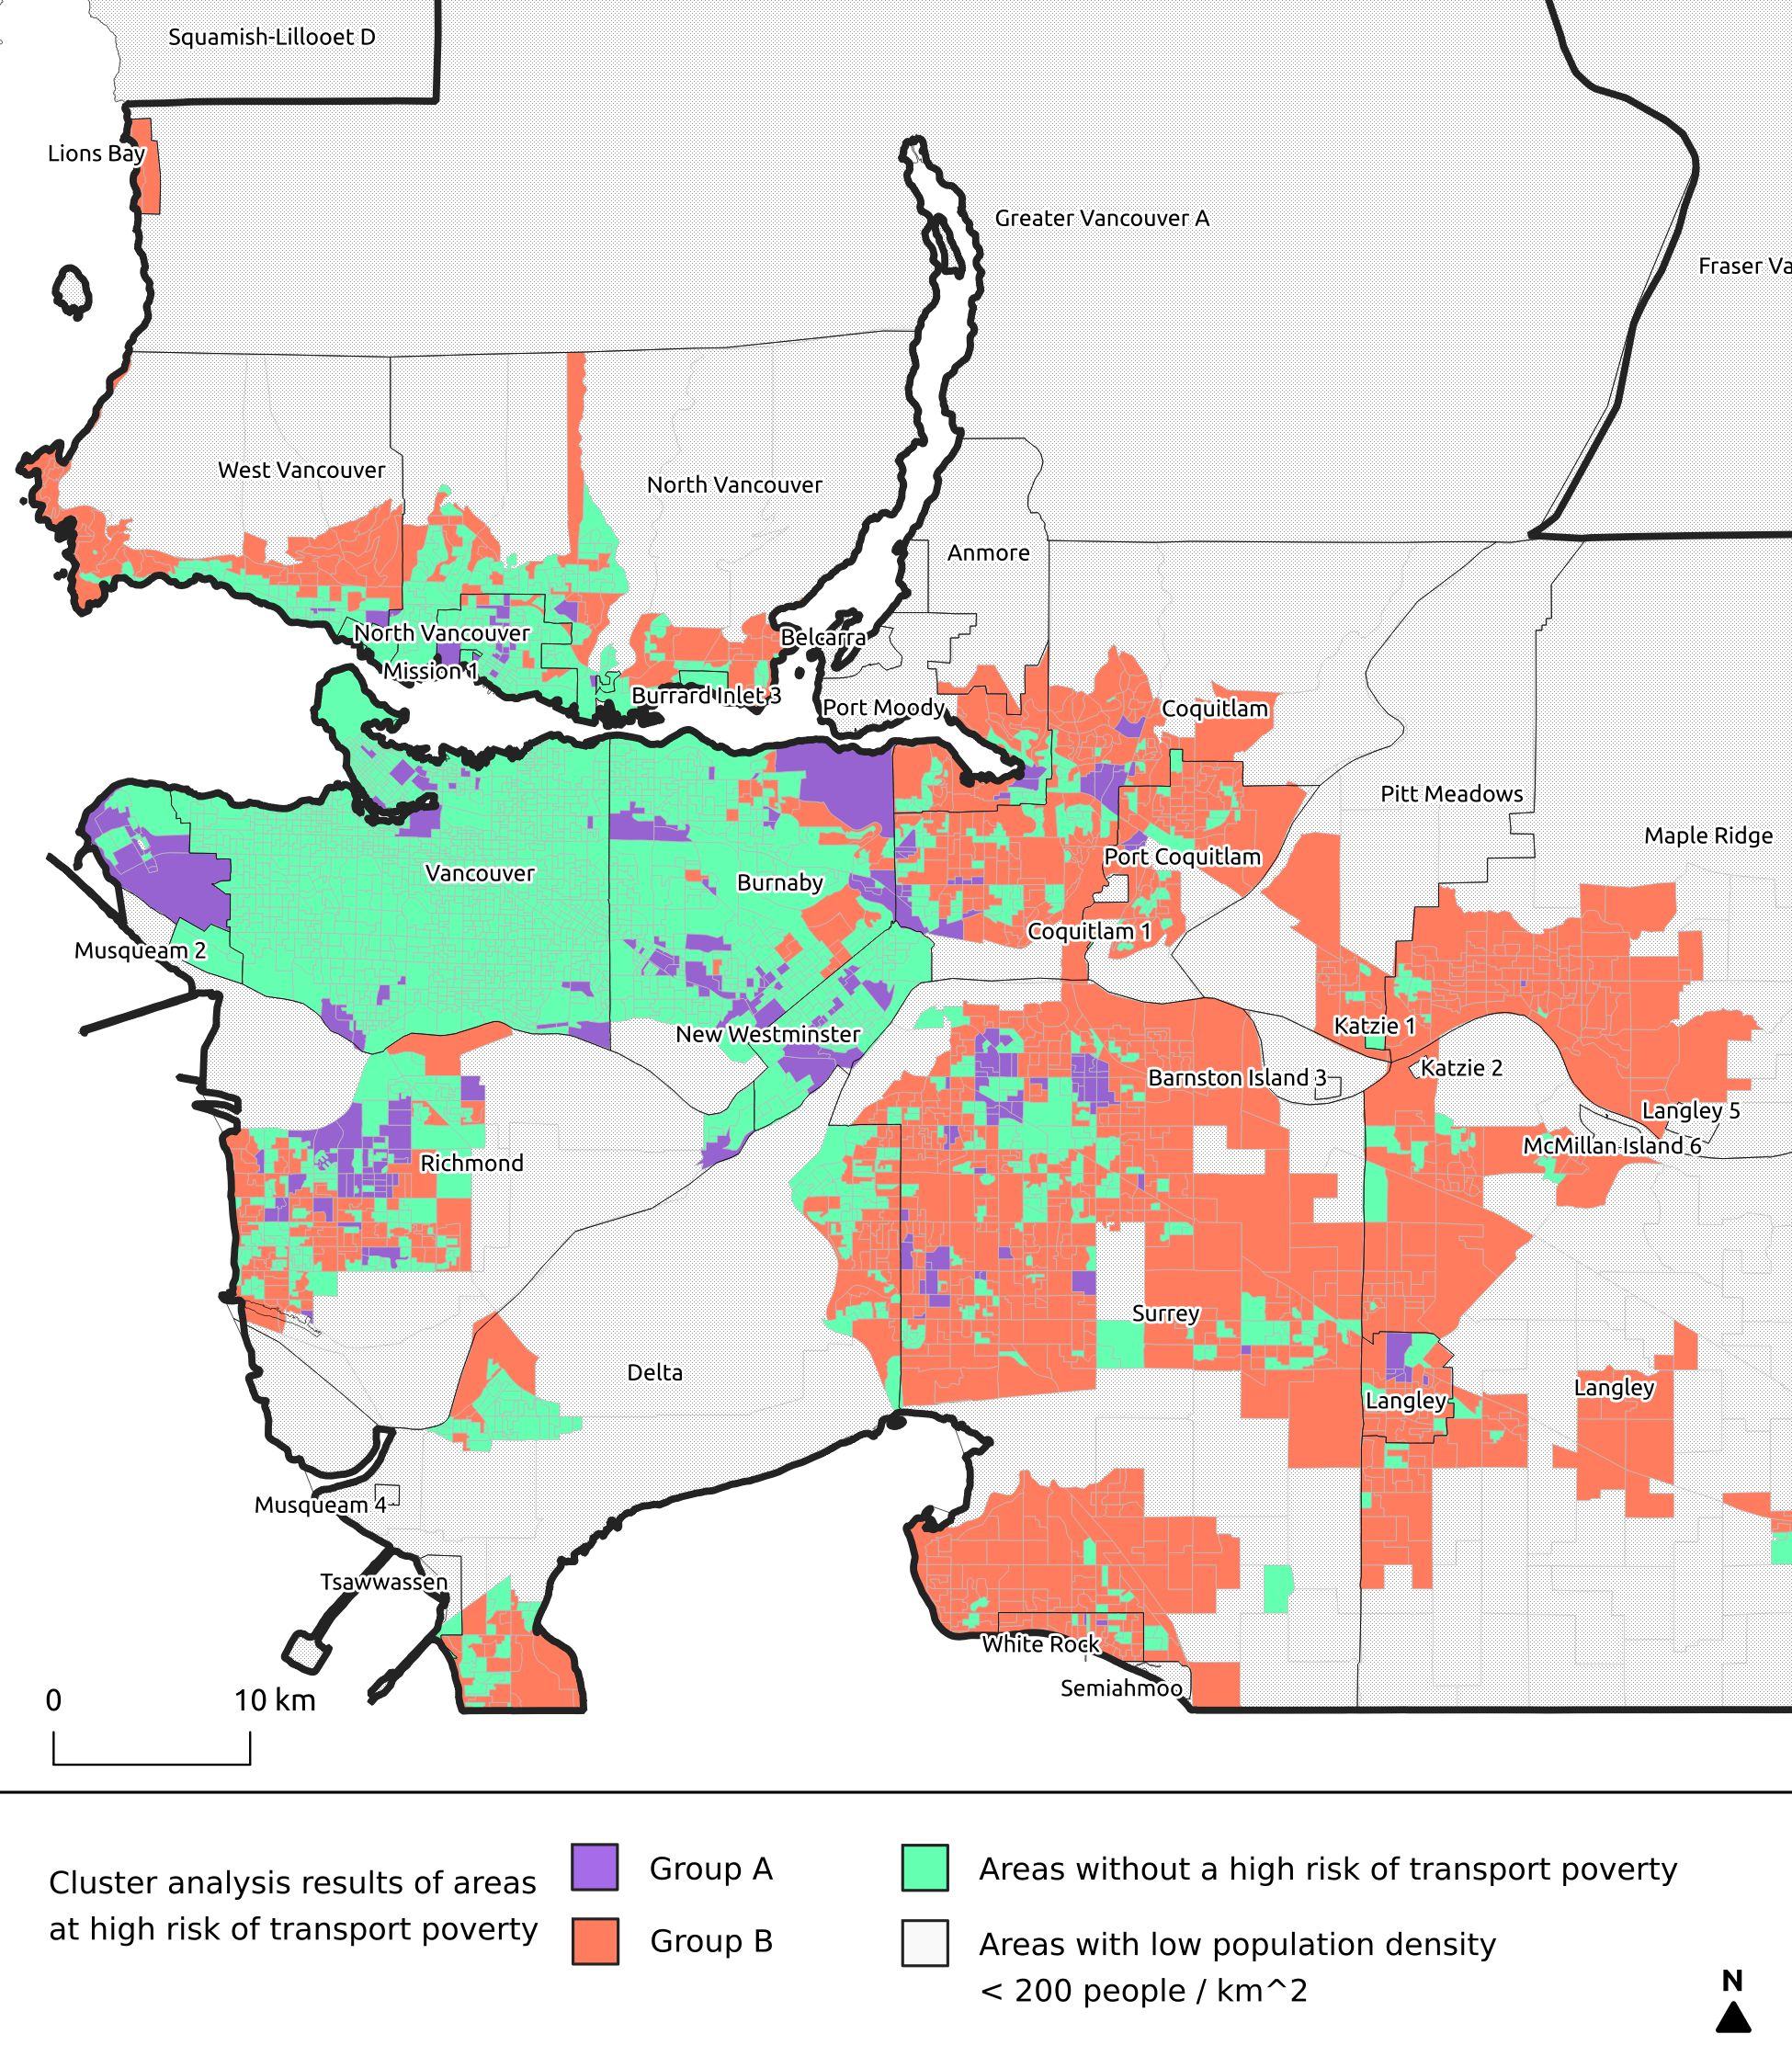
\includegraphics[width=6.5in]{figures/cluster_maps/C_van}}
	\vspace{2mm}
\end{figure}




\end{document}